z\documentclass[a4paper,12pt,twoside]{book}
\usepackage[utf8]{inputenc}
\usepackage[english]{babel}
\usepackage{fancyhdr}
\setlength{\headheight}{52pt}
\usepackage{graphicx}
\usepackage{amsmath}
\usepackage{amssymb}
\usepackage{amsfonts,bm}
\usepackage{empheq}
% \usepackage{cmbright}
% \usepackage{textcomp}
\usepackage{centernot}
\usepackage{authblk}
\usepackage{hyperref}

\usepackage{mathpazo} 


\usepackage[usenames,dvipsnames,svgnames,table]{xcolor}
\pagecolor{white}
\pagestyle{fancy}
\fancyhf{}
\fancyhead[LE,RO]{Scientific Computing}
\fancyhead[RE,LO]{\thepage}
\fancyfoot[CE,CO]{\leftmark}
\fancyfoot[LE,RO]{}

\newcommand*\widefbox[1]{\fbox{\hspace{2em}#1\hspace{2em}}}

\usepackage{mathtools}
\newcommand{\bb}[1]{\mathbb{#1}}
\newcommand{\nll}[0]{\newline\newline}
\newcommand{\tit}[1]{\textit{#1}}
\newcommand{\theor}[1]{\boxed{\textbf{\textit{Theorem \thechapter.#1}}}}
\newcommand{\algo}[0]{\boxed{\textbf{\textit{Algorithm}}}}
\newcommand{\assum}[0]{\boxed{\textbf{\textit{Assumption}}}}
\newcommand{\formula}[0]{\boxed{\textbf{\textit{Formula}}}}
\newcommand{\defin}[0]{\boxed{\textbf{\textit{Definition}}}}
\DeclarePairedDelimiter\abs{\lvert}{\rvert}
\newcommand{\vect}[1]{\bm{#1}}
\newcommand{\mat}[1]{\bm{\mathrm{#1}}}
\newcommand{\norm}[1]{\Vert #1 \Vert}
\newcommand{\innerp}[2]{\langle #1, #2 \rangle}
\newcommand{\expec}[1]{\mathbb{E}\left[ #1 \right]}
\newcommand{\seq}[1]{\left\{#1\right\}}
\newcommand{\pder}[2]{\frac{\partial #1}{\partial #2}}
\newcommand{\der}[2]{\frac{d #1}{d #2}}
\newcommand{\estif}[1]{\hat{\theta}\left( #1 \right)}
\newcommand{\esti}[0]{\hat{\theta}}
\newcommand{\bpder}[3]{\left( \pder{#1}{#2}\right)_{#3}}
\renewcommand{\d}[0]{\prime}

\newcommand{\chapterendsymbol}{
	\par
	\vspace{\stretch{1}}
	\begin{figure}[htbp]
	\begin{center}
		
\includegraphics[width=0.5\textwidth]{BookEnd.pdf}
	\end{center}
\end{figure}
	\vspace{\stretch{2}}
}


\hypersetup{
	colorlinks,
	citecolor=black,
	filecolor=black,
	linkcolor=black,
	urlcolor=black
}

\title{Lecture Notes in Scientific Computing MA311-M}
%\author{Instructor - Prof. Rajen Kumar Sinha}
%\author[1]{Prof. Rajen Kumar Sinha}
\author{Animesh Renanse}
\affil{Department of Electrical \& Electronics Engineering, Indian Institute of Technology, Guwahati}
\begin{document}

	\maketitle
	\thispagestyle{empty}
	\tableofcontents
\chapter{Introduction}
\section{Lecture 0 : Course Introduction}
\textbf{\textit{Date : September 4, 2020}}
\newline\newline
We'll be learning about various numerical techniques to solve some difficult problems arising in Engineering. We need a measure to analyze performance of such methods, thus performance analysis. Then we also need to design these computational procedures formally and then implement them on a computing machine.
\subsection{Course Overview and References}
\begin{itemize}
	\item {Iterative methods for non-linear equations, interpolation, numerical differentiation and integration, one step and multi-step methods for ODEs and numerical solutions of PDEs by Finite Difference Methods (FDMs).}
	\item{Kincaid and Cheney; Numerical Analysis: Mathematics of Scientific Computing }
	\item{G.D. Smith, Numerical Solutions of Partial Differential Equations}
	\item{\textbf{Software Requirements : }MATLAB}
\end{itemize}
\subsection{Evaluation Policy}
\begin{itemize}
	\item {Two assignments : each 10\% }
	\item{Two quizzes : each 10\%}
	\item{Four assignments : each 5\%}
	\item{Viva Voce : each 10\%}
	\item{End Semester exam : 30\%}
\end{itemize}
\textbf{Weekly Meeting for questions: Every Friday 10 AM - 10:55 AM}
\chapter{Errors in Numerical Computation}
\textbf{Lecture 2, \textit{September 9, 2020}}
\newline\newline
\section{Real Numbers, Machine Numbers, Rounding}
True values are not stored exactly in a computer, it always undergo a rounding or chopping, and additional operators introduce more errors.
\newline\newline
\textbf{Real Numbers: } We adopt \textbf{binary number system}.
\begin{equation*}
	\begin{split}
		x &\in \mathbb{R}\\
		x &= \pm \left( b_n 2^{n} + b_{n-1}2^{n-1} +\cdots \right) 
	\end{split}
\end{equation*}
where $n$ is some integer and the  \textbf{binary digits $b_i$} takes the value either 0 or 1. Hence we can write in general that,
\begin{equation*}
	\begin{split}
		x = \pm\left( b_n b_{n-1} \cdots b_0 b_{-1} b_{-2} \cdots \right) _2
	\end{split}
\end{equation*}
to remind us that we are dealing with binary numbers.
\newline\newline
\textbf{Remark: } It's not true that a finite decimal number will have a finite representation in a binary computer. However, to a finite binary number there always corresponds a finite decimal representation.
\newline\newline
\textbf{Machine Numbers:} Two kinds,
\begin{itemize}
	\item {Floating-point number}
	\item{Fixed-point number}
\end{itemize}
\subsubsection{Floating Point number}
Let $\mathbb{R}\left( t,s \right) $ be the set of \textbf{real} floating point numbers on a computer, it implies that if,
\begin{equation*}
	\begin{split}
		x\in  \mathbb{R}\left( t,s \right) \; \text{ implies and is implied by } \; \boxed{x = f.2^{e}}
	\end{split}
\end{equation*}
where, 
\begin{equation*}
	\begin{split}
		f = \pm\left( b_{-1}b_{-2}\cdots b_{-t} \right)_2 \;,\;\; e=\pm \left( c_{s-1} c_{s-2} \cdots c_0 \right)_2
	\end{split}
\end{equation*}
Here, $t$ is the number of binary digits allowed by the computer in the fractional part and  $s$ is the number of binary digits in the exponent.  \textbf{$f$ is referred as the mantissa and  $e$ is referred to as the exponent of  $x$}.
\newline\newline
\boxed{\textbf{\textit{Formula}}} : The \textbf{largest} and \textbf{smallest} magnitude of a floating point number is given by,
\begin{equation}
	\label{min-max-magn}
	\begin{split}
		fl_{max}\left( x \right) &=  \underset{x \in \mathbb{R}\left( t,s \right) } {\text{max}} \vert x\vert = \left( 1-2^{-t} \right) 2^{2^{s}-1}\\
		fl_{min}\left( x \right) &=  \underset{x \in  \mathbb{R}\left( t,s \right) }{\text{min}} \vert x \vert = 2^{-2^{s}}
	\end{split}
\end{equation}
The trivially used terms \textbf{\textit{overflow}} and \textbf{\textit{underflow}} refers to the respective cases when during the course of the computation the number produced have a modulus greater than $fL_{max}$ and less than $fl_{min}$.
\newline
However, we can still increase the precsion of the computation by introducing twice the number of allowed digits in the mantissa, i.e. $\mathbb{R}\left( 2t,s \right) $, this is called \textbf{double-precision number}.
\newline\newline
\textbf{Fixed Point number}
\newline\newline
This is just the special case that $\boxed{x=f \implies e=0}$.
\subsection{Rounding}
Let,
\begin{equation*}
	\begin{split}
		x \in \mathbb{R},\;\; x = \pm \left( \sum_{k=1}^{\infty} b_{-k}2^{-k} \right) 2^{e}
	\end{split}
\end{equation*}
be the exact real number in floating point form, thus the \textbf{rounded number} is,
\begin{equation}
	\begin{split}
		\boxed{x\in \mathbb{R},\;\;\pm\left( \sum_{k=1}^{t} b^{*}_{-k}2^{-k} \right) 2^{e^{*}}}
	\end{split}
\end{equation}
Now, two types of rounding are possible,
\begin{itemize}
	\item {\textbf{Chopping}: $x=\text{chop}\left( x \right)$, it implies that 
		\begin{equation*}
			\begin{split}
				e^{*} &=  e\\
				b^{*}_{-k}&= b_{-k}
			\end{split}
		\end{equation*}
		for all $k = 1,2,\cdots,t$.
	}
\item{\textbf{Symmetric rounding}: The rounding up or rounding down in decimal arithmetic based on the first discarded digit. Example, If the discarded digit $\ge 5$, then we round up and otherwise.
\newline\newline
\textbf{Note: } In binary arithmetic, \textbf{if the first discarded binary digit is 1 then we round up and if it is 0, then we round down}.
	}
\end{itemize}
More concretely, we can write the \textbf{chop} and \textbf{rd} operation as the following,
\begin{equation}
	\begin{split}
		x &= \text{rd}\left( x \right)\\
		\text{rd}\left( x \right) &= \text{chop}\left( x + \underbrace{\frac{1}{2}\;.\;2^{-t}\;.\;2^{e}}_{ \text{adds $\frac{1}{2}$ to  make it compatible}} \right) 
	\end{split}
\end{equation}
In the case of \textbf{chopping}, the \textbf{absolute error} can be calculated as,
\begin{equation}
	\begin{split}
		\abs{x - \text{chop}\left( x \right) } &=  \abs*{\pm \sum_{k=t+1}^{\infty} b_{-k}2^{-k}}2^{e}\\
		&\boxed{\le \sum_{k=t+1}^{\infty} 2^{-k} \;.\; 2^{e} = 2^{-t}\;.\;2^{e}} 
	\end{split}
\end{equation}
Similarly, we can calculate the \textbf{relative error} in the case of chopping as,
\begin{equation}
	\begin{split}
		\abs*{\frac{x-\text{chop}\left( x \right) }{x}} &\le \frac{2^{-t}2^{e}}{\abs*{\pm \sum_{k=1}^{\infty} b_{-k}2^{-k}}2^{e}} \\
		&\le \frac{2^{-t}2^{e}}{ \underbrace{\frac{1}{2}\;\;.\;\;2^{e}}_{\text{this is minimized}}}\\
		&\boxed{\le 2 \;.\; 2^{-t}}
	\end{split}
\end{equation}
$\star$ Note that the \textbf{upper bound on the relative error is not dependent on $e$.}
\newline\newline
$\star\star$\textbf{Remark: }The machine dependent term $\boxed{\text{eps} = 2^{-t}}$ is also called the \textbf{machine precision} . 
\newline\newline
Similarly, for the \textbf{rounding}, we can find the relative error to be upper bounded by the following inequality,
\begin{equation}
	\begin{split}
		\boxed{\abs*{\frac{x - \text{rd}\left( x \right) }{x}}\le 2^{-t}}
	\end{split}
\end{equation}
for convenience, we write this in the following equivalent form,
\begin{equation}
	\begin{split}
		\boxed{\text{rd}\left( x \right) = x\left( 1+\varepsilon \right)\;,\;\;\;\abs*{\varepsilon} \le \text{eps}} 
	\end{split}
\end{equation}
\subsection{Machine Arithmetic}
\defin  : \textit{Let $\circ$ denote arithmetic operation $\left( =,+,-,\times ,/ \right) $. Let $x,y \in \mathbb{R}\left( t,x \right) $ and let $fl\left( x\circ y \right) $ denote the machine produced result of the arithmetic operation, then,
\begin{equation}
	\begin{split}
		fl\left( x\circ y \right) = x \circ y\left( 1+\varepsilon \right) \;,\;\;\abs{\varepsilon} \le \text{eps}
	\end{split}
\end{equation}
}
\subsubsection{Multiplication}
Consider values $x\left( 1+\varepsilon_x \right) $ and $y\left( 1+\varepsilon_y \right) $ of $x$ and $y$ \textit{contaminated} by relative errors $\varepsilon_x$ and $\varepsilon_y$ respectively, in this case, the \textbf{relative error in the product is,}
\begin{equation*}
	\begin{split}
		&\text{rd}\left( x.y \right) \approx xy\left( 1+ \varepsilon_x+\varepsilon_y\right) \\
	\implies & \abs*{\frac{xy - \text{rd}\left( xy \right)}{xy} } \approx \varepsilon_x+\varepsilon_y\\
&\boxed{\varepsilon_{x.y}=\varepsilon_x + \varepsilon_y} 
	\end{split}
\end{equation*}
where we neglect higher order interaction terms of error in product.
\subsubsection{Division}
\begin{equation*}
	\begin{split}
		\frac{x\left( 1+\varepsilon_x \right) }{y\left( 1+\varepsilon_y \right) } = \frac{x}{y} \left( 1+\varepsilon_x \right) \left( 1-\varepsilon_y+\varepsilon_y^2-\dots \right) \\
		\approx \frac{x}{y} \left( 1+\varepsilon_x-\varepsilon_y \right) 
	\end{split}
\end{equation*}
therefore,
\begin{equation*}
	\begin{split}
		\boxed{\varepsilon_{\frac{x}{y}} = \varepsilon_x - \varepsilon_y}
	\end{split}
\end{equation*}
\subsubsection{$\star$Addition and Subtraction}
\begin{equation*}
	\begin{split}
		x\left( 1+\varepsilon_x \right) + y\left( 1+\varepsilon_y \right) &= \left( x+y \right) \left( 1+\frac{x\varepsilon_x + y\varepsilon_y}{x+y} \right)\;,\;\; x+y\neq 0
	\end{split}
\end{equation*}
Therefore, we have the interesting case that,
\begin{equation}
	\label{add-err}
	\begin{split}
		\boxed{\varepsilon_{x+y} = \frac{x}{x+y}\varepsilon_x + \frac{y}{x+y}\varepsilon_y}
	\end{split}
\end{equation}
Therefore, now the relative error also depends on the inputs! Thus the addition is a  \textbf{benign} operation. The error in Eq. \ref{add-err} is called \textbf{cancellation error}. This type of \textbf{cancellation error should be avoided in the calculations as much as possible, thus try to avoid addition and subtraction directly as much as possible.}
\newline\newline
\textbf{Example 2: } \textit{If $y = \sqrt{x+\delta} - \sqrt{x} $, $x>0$,  $\abs{\delta}$ is very small. To avoid cancellation error, one should write
\begin{equation*}
	\begin{split}
		y = \frac{\delta}{\sqrt{x+\delta} + \sqrt{x} }
	\end{split}
\end{equation*}
}
\textit{Thus finding equivalent representations is an important concept for direct Addition and Subtraction as concretely shown in above example (and in slides).}

\chapter{The Solution of Non-Linear Equations by Bisection Method}
We want to find the real root of the following type of equations,
\[f(x) = 0\]
where $f:[a,b] \rightarrow \bb{R}$. Here the function $f(x)$ might be any of the following,
\begin{itemize}
    \item {a polynomial in $x$}
    \item{a transcendental function }
    \item{any combination of the above two.}
\end{itemize}
There is no closed form method to find solutions to such equations, like the following
\[e^{-x} - \sin x = 0\]
Thus to solving these, one \textbf{has to look for approximate methods}.
\nll
Note that before asking the question that \tit{what are the solutions of $f(x)$}, we should first answer the question that \tit{whether there exists solutions of $f(x) = 0$ or not.} In that extent, we  have the following theorem,
\nll
\theor{0}   : \tit{(Bolzano's Theorem) Assume that $f \in C[a,b]$ and $f(a)f(b)<0$. Then there exists atleast one number $r\in(a,b)$ such that $f(r) = 0$.}
\section{The Bisection Method}
Given $f\in C[a,b]$ be such that $f(a_0)f(b_0) < 0$, then the bisection method can be explained by the following algorithm,
\nll
\algo
\nll
For $n=0,1,2,...$ do:
\begin{enumerate}
    \item {Set $c_n = \frac{a_n + b_n}{2} $.}
    \item {If $\abs*{f(c_n)} < \epsilon$ (\tit{prescribed tolerance}), then \textbf{accept $c_n$}, STOP.}
    \item{If $f(a_n)f(c_n) < 0$, then \textbf{set} $a_{n+1} = a_n$ and $b_{n+1} = c_n$, \textbf{goto} Step 1.  }
    \item{else \textbf{set} $a_{n+1} = c_n$ and $b_{n+1} = b_n$, \textbf{goto} Step 1.}
\end{enumerate}

\textbf{Remark : }To avoid cancellation error, compute the mid-point $c_n$ instead as the following,
\[ c_n = a_n + \frac{b_n -a_n}{2} \]
\section{Error Analysis}
Let $[a_0, b_0], [a_1, b_1], \cdots$, be successive intervals arising in the algorithm above with the following holding true,
\[a_0\le a_1 \le \cdots \le b_0 \;\; \text{and} \;\; b_0\ge b_1\ge \cdots \ge a_0\]
We thus have,
\[b_{n+1} - a_{n+1} = \frac{1}{2} (b_n - a_n)\]
Note that the sequence $\{a_n\}$ is bounded above and hence \textbf{converges} (\tit{increasing or decreasing sequence which is bounded}) . Similarly, $\{b_n\}$ also converges.
\nll
Since,
\[ \boxed{b_n - a_n = \frac{1}{2}(b_{n-1} - a_{n-1})= \cdots = \frac{1}{2^n}(b_0 - a_0)}\]
it thus follows that,
\[ \underset{n\to\infty}{\lim} b_n - \underset{n\to\infty}{\lim} a_n = \underset{n\to\infty}{\lim} \frac{1}{2^n}(b_0 - a_0)\]
\[\implies \underset{n\to\infty}{\lim} a_n = \underset{n\to\infty}{\lim} b_n = r\;\;(\text{\tit{say}})\]
Hence, we now see that
\[ \boxed{\underset{n\to\infty}{\lim} f(a_n)f(b_n) \le 0 \implies f^2(r) \le 0 \implies f(r) = 0} \]
But suppose we stop the process at the timestep $n$, thus we'll have the interval $[a_n,b_n]$. \tit{Then the best estimate of the root will clearly be $c_n = \frac{a_n + b_n}{2}$.} The error at this timestep $e_n$ will then be,
\[ \boxed{e_n = \abs*{r - c_n} \le \underbrace{\frac{1}{2}(b_n - a_n)}_{\text{len of half inter.}} = \frac{1}{2^{n+1}}(b_0 - a_0) } \]
\theor{1}    : \tit{Assume that $f \in C[a,b]$. Let $[a_0,b_0], [a_1,b_1], \cdots, [a_n,b_n],\cdots$ denotes the intervals in the bisection method. Then $\underset{n\to\infty}{\lim} a_n$ and $\underset{n\to\infty}{\lim} b_n$ \textbf{exists, are equal and represent a zero of $f$}. If $r = \underset{n\to\infty}{\lim} c_n$, where $c_n = \frac{a_n + b_n}{2}$, then,
\[ \abs*{r - c_n} \le 2^{-(n+1)} (b_0 - a_0) \]
}

\chapter{Newton-Raphson Method}
We will first introduce the method for single variable function and then we will extend it to non-linear functions.
\nll
Let $x_0$ be an initial approximation to $r$ and let $h$ be the \textbf{correction} given to $x_0$ such that 
\[f(x_0 + h) = 0\]
\assum  : We assume that $f^{\prime}(x)$ exist and is continuous.
\nll
Now, by Taylor's theorem,
\[0 = f(x_0 + h) = f(x_0) + hf^\prime (x_0) + \text{higher order terms ...}\]
Neglecting the higher order terms for sufficiently small $h$ (\textit{note that we are hence linearizing the original equation}), we simply get 
\[h = -\frac{f(x_0)}{f^\prime(x_0)}\]
Hence the \tit{first approximation to the exact root} is given by
\[x_1 = x_0 - \frac{f(x_0)}{f^\prime(x_0)} \]
Now we repeat the above procedure by substituting our initial approximation to be $x_1$. Hence setting $x_0 \leftarrow x_1$ and repeat the above procedure to have,
\[h = - \frac{f(x_1)}{f^\prime(x_1)}\]
and obtain the second approximation as 
\[x_2 = x_1 - \frac{f(x_1)}{f^\prime(x_1)}\]
In general,after $n^{th}$ step an approximaion to the exact root becomes,
\[\boxed{x_{n+1} = x_n - \frac{f(x_n)}{f^\prime(x_n)}\;,\;\;\;\;n\ge 0}\]
which is the \textbf{Newton-Raphson Method}.
\section{Geometric Interpretation}
The $n^{th}$ approximation of the root by the Newton-Raphson's method is given geometrically by drawing the tangent to $f(x)$ at the point $x_{n}$ and determining the point of intersection of input axes ($X$-axis in the case of single variable functions) with this tangent.
\nll
More concretely, the equation of the tangent to $f$ at $(x_0, y_0)$ is given by,
\[y - f(x_0) = f^\prime (x_0) ( x-x_0)\]
Now the above tangent line meets the $x$-axis at $y=0$, which gives us,
\[x_1 \approx x = x_0 - \frac{f(x_0)}{f^\prime(x_0)}\]
which is just the first approximation.
\section{Error Analysis}
We need some definitions before diving into analysis of Newton's method.
\nll
\defin  : \tit{(Order of Convergence) Let $\{x_n\}$ be a sequence of real numbers tending to a limit $r$ and set $e_n = x_n - r$. \textbf{If} there exists a number $p$ and a constant $C>0$ such that
\[ \underset{n\to \infty}{\lim} \frac{\abs*{e_{n+1}}}{\abs*{e_n}^p} = C\]
then $p$ is called the \textbf{order of convergence of the sequence $\{x_n\}$} and $C$ is called the \textbf{asymptotic error constant}}.  
\nll
Now, let $r$ be a root of $f(x) = 0$. Let $x_n$ be the approximation to $r$ obtained by the Newton Raphson's method after the $n^{th}$ iteration. Defining the error $e_n = r - x_n$, we thus get,
\[0 = f(r) = f(x_n +(r-x_n))\\
= f(x_n) + (r-x_n)f^\prime(x_n) + \frac{(r-x_n)^2}{2}f^{\prime\prime} (\eta_n)
\]
where $\eta_n$ lies between $r$ and $x_n$. Now solving for $r$ from the above equations gives us
\begin{equation*}
    \begin{split}
        r &= x_n -  \frac{f(x_n)}{f^\prime(x_n)} - \frac{(r - x_n)^2}{2} . \frac{f^{\prime\prime}(x_n)}{f^\prime(x_n)}\\
        &= x_{n+1} - \frac{(r - x_n)^2}{2} . \frac{f^{\prime\prime}(x_n)}{f^\prime(x_n)}
    \end{split}
\end{equation*}
hence the $r-x_{n+1} = e_{n+1}$ is given by,
\begin{equation*}
    \begin{split}
        e_{n+1} = -\frac{e_n^2}{2} . \frac{f^{\prime\prime}(x_n)}{f^\prime(x_n)} \approx -\frac{1}{2} \frac{f^{\prime\prime}(r)}{f^\prime(r)} e^2_n =Ce_n^2
    \end{split}
\end{equation*}
Hence, the \textbf{Newtons's method converges quadratically.}
\nll
\textbf{NOTE: } Newton's method yields quadratic convergence only under the following assumptions
\begin{enumerate}
    \item {$r$ is a simple root of $(x) = 0$, i.e. $r$ should not be a repeated root of $f$.}
    \item{$f^\prime(x) $ should not be too small in the neighborhood of he initial choice $x_0$, otherwise the steps taken would be too high for convergence.}
    \item{The initial approximation $x_0$ should be chosen very close to the root, as there are examples, like piecewise defined functions in which $f^\prime(x_0)$ could be zero, and hence again, the steps would be infinitely large.}
\end{enumerate}
 But under certain conditions, we can concretely say that the Newton's method converges to a root, as stated in the following theorem.
 \nll
 \theor{2}  : \tit{Let $f \in C^2([a,b])$ and the following conditions be satisfied:
 \begin{enumerate}
     \item {$f(a)f(b) < 0$.}
     \item{$f^\prime(x) \neq 0 \; \; \forall \; \; x \in [a,b]$.}
     \item{$f^{\prime\prime} (x)$ is either $\ge 0$ or $\le 0$ for all $x \in [a,b]$.}
     \item{At the endpoints $a$ and $b$,
     \[\frac{\abs{f(a)}}{\abs{f^\prime(a)}} < b-a \;\; \text{and} \;\; \frac{\abs{f(b)}}{\abs{f^\prime(b)}} < b-a\]
     }
 \end{enumerate}
 Then the Newton's method converges to the unique root $r$ of $f(x)=0$ in $[a,b]$ for \textbf{any} starting value $x_0 \in [a,b]$.
 }
 \nll
 \textbf{REMARK : } The regularity conditions implies the following,
 \begin{itemize}
     \item {Bolzano's Theorem, there exists atleast one root of $f(x) = 0$ in $[a,b]$.}
     \item{Since the function $f$ is now strictly increasing or decreasing, then there exists only one solution in the interval $[a,b]$.}
     \item{Since the function is now either concave from upward or downward, thus the derivative $f^\prime$ is either increasing or decreasing in $[a,b]$.}
     \item{To make sure the step size isn't more than the size of the interval itself.}
 \end{itemize}
\chapter{System of Non-Linear Equations}
We extend the Newton's linearization technique now to system of non-linear equations. For that aim, we first consider system of two variables and then extend the same idea to any system of $n$ variables.
\nll
Consider the system of two non-linear equations in two independent variables $x_1$ and $x_2$ as,
\[f_1(x_1,x_2) = f_2(x_1,x_2) = 0\]
Let $(x_1^0, x_2^0)$ be the \textbf{initial approximation} to the exact solution and let the $h_1^0$ and $h_2^0$ be the \textbf{corrections} given to $x_1^0$ and $x_2^0$ respectively so that,
\[ f_1(x_1^0 + h_1^0, x_2^0 + h_2^0) = f_2(x_1^0 + h_1^0, x_2^0 + h_2^0) = 0\]
Then \textbf{using Taylor's expansion upto linear terms} would yield
\begin{equation*}
    \begin{split}
        f_1(x_1^0 + h_1^0, x_2^0 + h_2^0) &\approx f_1(x_1^0, x_2^0) + h_1^0 \frac{\partial f_1}{\partial x_1^0} + h_2^0 \frac{\partial f_1 }{\partial x_2^0}\\
        f_2(x_1^0 + h_1^0, x_2^0 + h_2^0) &\approx f_2(x_1^0, x_2^0) + h_1^0 \frac{\partial f_1}{\partial x_1^0} + h_2^0 \frac{\partial f_1 }{\partial x_2^0}
    \end{split}
\end{equation*}
where the partial derivatives are evaluated at $(x_1^0, x_2^0)$.
\nll
Rewriting the above equation in the matrix form,
\begin{equation*}
\mathbf{J}\mathbf{h} = -\mathbf{f}
\end{equation*}
where $\mathbf{J}$ is the  \textbf{Jacobian matrix} $\mathbf{J}(f_1, f_2)$, the \textbf{correction vector} $\mathbf{h}$ and the vector $\mathbf{f}$ are given by,
\begin{equation*}
    \begin{split}
        \mathbf{J} &= \begin{bmatrix} \frac{\partial f_1}{\partial x_1^0} & \frac{\partial f_1}{\partial x_2^0} \\
        \frac{\partial f_2}{\partial x_1^0}&
        \frac{\partial f_2}{\partial x_2^0}\end{bmatrix}\\
        \mathbf{h} &= \begin{bmatrix} h_1^0 \\ h_2^0 \end{bmatrix}\\
        \mathbf{f} &= \begin{bmatrix} f_1(x_1^0, x_2^0)\\f_2(x_1^0, x_2^0)
        \end{bmatrix}
    \end{split}
\end{equation*}
\textbf{If $\mathbf{J}$ is invertible}, then the correction vector $\mathbf{h}$ is determined simply by,
\[ \boxed{\mathbf{h} = - \mathbf{J}^{-1} \mathbf{f} }\]
and then the \textbf{the first approximation} would simply become,
\[\boxed{x_1^1 = x_1^0 + h_1^0 \;\;\;, \;\;\; x_2^1 = x_2^0 + h_2^0}\]
and then we can repeat the whole method to get even finer approximations. Hence, more generally, we get,
\[ \begin{bmatrix} x_1^{n+1} \\ x_2^{n+1}\end{bmatrix} =  \begin{bmatrix} x_1^{n} \\ x_2^{n}\end{bmatrix} + \begin{bmatrix} h_1^{n} \\ h_2^{n}\end{bmatrix}\]
\nll
\textbf{Remark : } Few things to keep in mind are as follows,
\begin{itemize}
    \item {At \textbf{each} stage or timestep, we need to solve the following linear system,
    \[ \mathbf{J}  \begin{bmatrix} h_1^n \\ h_2^n \end{bmatrix} = - \begin{bmatrix} f_1(x_1^n, x_2^n)\\f_2(x_1^n, x_2^n)
        \end{bmatrix} \]
    }
    \item{The \textbf{Stopping Criterion} is, given the tolerance $tol$,
    \[ \abs{h_1^n} + \abs{h_2^n} < tol \]
    }
\end{itemize}
\section{Newton's Iteration on Non-Linear system of $n$ variables}
Now, we extend the idea introduced earlier for system of 2 variables to a more general $n$ variables.
\nll
Consider the system,
\[ \mathbf{f}(\mathbf{x}) = \mathbf{0} \]
where $\mathbf{f} = \begin{pmatrix} f_1, f_2, \dots, f_n \end{pmatrix}^T$ and $\mathbf{x} = \begin{pmatrix} x_1, x_2, \dots, x_n \end{pmatrix}^T$. 
\nll
The \textbf{linearization of above equation} thus yields the following,
\begin{equation}
    \mathbf{f}(\mathbf{x} + \mathbf{h}) \approx \mathbf{f}(\mathbf{x}) + \mathbf{f}^\prime (\mathbf{x}) \mathbf{h}
\end{equation}
where the $n$ long \textbf{correction vector} $\mathbf{h} = \begin{pmatrix} h_1, h_2, \dots, h_n \end{pmatrix}^T$ and the \textbf{Jacobian matrix of $\mathbf{f}$} is,
\[ \mathbf{f}^\prime (\mathbf{x}) = \mathbf{J} = \begin{bmatrix} \frac{\partial f_1}{\partial x_1}& \cdots & \frac{\partial f_1}{\partial x_n}\\ \vdots & \ddots & \vdots \\ \frac{\partial f_n}{\partial x_1} & \cdots & \frac{\partial f_n}{\partial x_n}   \end{bmatrix} \]
Then, the correction vector $\mathbf{h}$ is simply obtained by,
\begin{equation}
    \boxed{\mathbf{h} = - \mathbf{J}^{-1} \mathbf{f}(\mathbf{x})}
\end{equation}
after this, we simply get the iteration formula as,
\begin{equation}
\begin{split}
    \mathbf{x}^{n+1} &= \mathbf{x}^n + \mathbf{h}^n\\
    \mathbf{h}^n &= -\mathbf{J}^{-1} \mathbf{f}(\mathbf{x}^n) 
    \end{split}
\end{equation}
Hence, the whole process can be simply stated as the following,
\nll
\textbf{\tit{Retrieve the initial point for the current timestep, then calculate the correction vector for this timestep by solving the 5.2, add this correction to the initial point to get the new approximation, substitute the new approximation as the initial approximation for the next timestep. Stop when the $n^{th}$ power of $l_n$ norm of correction vector is less than the tolerance $tol$ hyperparameter.}}

\chapter{The Fixed-Point Method}
In this chapter, we look at a new method for computing the roots of a non-linear function using the properties of it's fixed point.
\section{Fixed Point of a function}
\defin  : \tit{(Fixed Point) Let $f : \mathbb{R} \to \mathbb{R}$ be a real valued function. A point $x_0$ is called a fixed point of $f$ if $f(x_0) = x_0$.}
\nll
Note that the equation $f(x) = 0$ can be put in the following form,
\[ x = g(x) \]
with which, we can thus conclude that \textbf{any fixed-point of $g$ above is a solution of $f(x) = 0$}.
\nll
For example, consider the function $f(x) = x^2 - x - 2$. Then, the possible choices for $g(x)$ are as follows,
\begin{itemize}
    \item{$g(x) = x^2 - 2$} 
    \item{$g(x) = \sqrt{x+2}$}
    \item{$g(x) = 1 + \frac{2}{x}$}
    \item{$g(x) = x - \frac{x^2 - x - 2}{m} \;,\;\;m\neq 0$} 
\end{itemize}
We hence get the following definition,
\nll
\defin  : \tit{(Iteration Function) A function $g(x)$ is called an iteration function for another function $f(x)$, if 
\[g(x) = x\]
implies $f(x) = 0$.
}
\nll
Note that we have effectively reduced our problem of determining the solution of $f(x) = 0$ to the problem of determining a fixed point of the function $g(x)$. Hence we just need to find the fixed point of the particular iteration function to yield us the solution of $f(x) = 0$. For this particular task, we thus have the following algorithm,
\nll
\algo :-
\begin{enumerate}
    \item {Given an iteration function $g(x)$ and a starting point $x_0$, compute
    \[ x_{n+1} = g(x_n) \;,\;\;\; n = 0,1,2,\dots\]
    until $\abs{x_n - r} < \epsilon$ ($eps$ is the hyperparameter $\verb|tolerance|$.).
    }
\end{enumerate}
Note that to implement the above algorithm, one needs to ensure the following,
\begin{itemize}
    \item {For given $x_0$, we \textbf{should} be able to generate $x_1, x_2, \dots$.}
    \item{Sequence $\{x_n\} \to r$.}
    \item{$r$ is a fixed point of $g(x)$, thus, $r = g(r)$.}
\end{itemize}
A natural question which thus arises is that whether the above algorithm will guarantee to find the fixed point of $g$ (thus, finding solution of $f(x) = 0$ in the process), for that purpose, we have the following theorem.
\nll
\theor{3}  : \tit{(Existence of Fixed Point) Set $I = [a,b]$. Let $g(x)$ be an iteration function satisfying the following conditions,
\begin{enumerate}
    \item {$g \; : \; I \to I$.}
    \item{$g\; : \; I \to I$ is continuous.}
    \item{$\exists$ a constant $0<K<1$ such that $\abs{g^\prime(x)} \le K$ for all $x \in I$}
\end{enumerate}
Then, $g(x)$ has a unique fixed point $r \in I$ and the sequence of iterations $\{x_n\}$ generated by $x_{n+1} = g(x_n)$ converges to $r$.
}
\nll
\tit{Proof : } Clearly, we first need to show there is a fixed point of $g$ in $I$. Note that if $g(a) = a$ or $g(b) = b$ then it's trivial. However in the case when $g(a)\neq a$ and $g(b) \neq b$, first note that $g(a),g(b) \in I$, so we can say that $g(a)>a$ and $g(b)<b$.
\nll
With this, we then define the following,
\[h(x) = g(x) - x\]
Clearly, $h(x) \in [0,b-a]$, therefore $h(a) > 0$ and $h(b)<0$ and since $h$ is continuous, thus by Bolzano's theorem, there is a point $r \in I$ such that $h(r) = 0$ which simply means that $g(r) = r$. Hence, there exists a fixed point of $g$ in $I$.
\nll
Now, to prove that the sequence of iterations generated by $x_{n+1} = g(x_n)$ converges to $r$, consider that at a particular instant of the iteration $n$, we are $\epsilon$ distance away from $r$, which is, consider,
\[r - x_n =  \epsilon\]
If we now calculate $\epsilon$,
\[\epsilon = r - x_n = g(r) - g(x_{n-1})\]
which can also be written via the first principle of derivative,
\[ \epsilon = r-x_n = g^\prime(\eta_n)(r-x_{n-1}) \]
for some $\eta_n$ between $x_n$ and $r$.
\nll
Now, for iterations to converge,
\begin{equation*}
    \begin{split}
        \abs{\epsilon_n} &\le K \abs{e_{n-1}}\\
        &\le K^2 \abs{e_{n-2}}\\
        &\le K^n \abs{e_0}
    \end{split}
\end{equation*}
Therefore, in the limit $n\to\infty$, since $K<1$, $e_n \to 0$. Which thus implies that $\{x_n\} \to r$.
\nll
Note that we also have to prove the \tit{uniqueness} of the fixed point, for that simply consider two points $r, r_1 \in I$ which are also fixed points, so, $g(r) = r$ and $g(r_1) = r_1$. If we set $x_0 = r$, then from the iteration,
\[x_1 = g(x_0) = g(r) = r\]
therefore, $e_0 = x_0 - r_1 = r-r_1$ and $e_1 = x_1 - r_1 = r-r_1$. But we know that $e_n \le K e_{n-1}$, therefore, we must have,
\[e_1 \le K e_0\]
Thus, we can conclude that $e_0 = e_1 = 0$, which simply implies that $r = r_1$.
\section{Performance Analysis}
We have the following theorem for the order of the convergence of the fixed point method.
\nll
\theor{4}  : \tit{Let $r$ be the root of $x = g(x)$. Assume that $g\in C^m(N_\delta (r))$ for $m\ge 2$ where $N_\delta(r)$ denotes a neighbourhood of $r$. Also assume that,
\[ g^\prime(r) = \dots = g^{(m-1)}(r) = 0\]
Then, if the initial guess $x_0 \in N_\delta(r)$, the iteration given by,
\[x_{n+1} = g(x_n)\;,\;\;\;n\ge 0\]
\textbf{converges with order $m$} and
\[\boxed{\underset{n\to \infty}{\lim} \frac{(r - x_{n+1})}{(r-x_n)^m} = \underbrace{(-1)^{m-1} . \frac{g^{(m)}(r)}{m!}}_{\text{finite value !}}}\]
}
\tit{Proof : } Consider the iteration,
\[ x_{n+1} = g(x_n)\]
We can expand it using Taylor's Theorem as follows,
\[x_{n+1} = g(x_n) = \sum_{k=0}^{m-1} \frac{(x_n - r)^k g^{(k)}(r)}{k!} + \frac{(x_n - r)^m g^{(m)}(\eta_n)}{m!}\]
Now, since $g^\prime(r) = \dots = g^{(m-1)}(r) = 0$, therefore,
\[x_{n+1} = r + \frac{(x_n - r)^m g^{(m)}(\eta_n)}{m!}\]
therefore,
\[\frac{x_n - r}{(x_n - r)^m} = \frac{g^{(m)}(\eta_n)}{m!}\]
finally, we get,
\[\frac{r - x_n}{(r-x_n)^m} = (-1)^{m-1}\frac{g^{(m)}(\eta_n)}{m!}\]

\chapter{Newton's Method from Fixed Point Method \& Multiple Roots}
We now analyze the Newton's method from Fixed Point method.
\nll
We know that the fixed point iteration algorithm for the iteration function of $f$ converges with order $m$ to a fixed point of the iteration function (refer to previous Theorem 6.4).
\nll
Now, recall the Newton's iteration,
\[ x_{n+1} = x_n - \frac{f(x_n)}{f^\prime(x_n)} \]
If we want to use fixed point method here, then we should have the following recurrence relation,
\[ x_{n+1} = g(x_n) \]
Comparing the above two equations, we thus get $g(x)$ as,
\[ g(x) = x - \frac{f(x_n)}{f^\prime(x_n)} \]
We can indeed verify that $g(x)$ has the fixed point as $r$ (the root of $f(x) = 0$),
\[ g(r) = r - \frac{f(r)}{f^\prime(r)} = r\]
Thus, now we have the \textbf{iteration function for Newton's Method}. To, however prove the convergence of Newton's method and convergence of iteration, we invoke Theorem 6.4.
\nll
For this task, we would need to check derivative of the iteration function $g$, thus,
\[g^\prime(x) = 1 - \frac{(f^{\prime}(x))^2 - f(x)f^{\prime\prime}(x)}{(f^\prime(x))^2} = \frac{f(x)f^{\prime\prime}(x)}{(f^\prime(x))^2}\]
Again, for $x=r$, we get $g^\prime$ as,
\[ g^\prime(x) = 0 \],
thus we observe that,
\[g(r) = r \;,\;\; g^\prime(r) = 0\;,\;\; g^{\prime\prime}(r) = \frac{f^{\prime\prime}(r)}{f^\prime(r)} \neq 0\]
Therefore \textbf{from Theorem 6.4, Newton's method has second order convergence}.
\section{Newton's method on Multiple Roots}
\defin  \;: (Root with multiplicity) \textit{If $r \in I$ is a root of $f(x)= 0$ with multiplicity $m>1$, then
\[f(x) = (x-r)^mh(x)\;,\;\; \text{where } h(x)\neq 0 \]
and $h(x)$ is continuous at $x=r$. Also, if $h \in C^m(I)$, then
\[ f(r) = f^\prime(r) = \dots = f^{(m-1)} = 0  \;\text{and}\; f^m(r) \neq 0\]}
Now, since we want to use Newton's method to find the root of $f(x) =0 $ where $f$ has root with multiplicity $>1$, thus we first need to find it's iteration function.
\nll
Note that since $f(x) = (x-r)^mh(x)$ and 
\[ f^\prime(x) = (x-r)^mh^\prime(x) + m(x-r)^{m-1}h(x) \]
thus, we get the iteration function (discussed previously for Newton's Iteration) $g(x)$ simply as,
\[g(x) = x - \frac{f(x)}{f^\prime(x)} = x - \frac{(x-r)^mh(x)}{(x-r)^mh^\prime(x) + m(x-r)^{m-1}h(x)} = \frac{(x-r)h(x)}{(x-r)h^\prime(x) + mh(x)}\]
Again, you can check that $g(x)$ has the fixed point as $r$, $g(r) = r$.
\nll
Now, to find the order of convergence of Newton's Method for function $f$ (which has root with higher multiplicity), we would again invoke the Theorem 6.4. Now to use this theorem, we need to find the amount of times we can differentiate $g$ and still get a continuous function which is not zero at the point $x=r$, so to check it, we start differentiating $g$ as follows,
\begin{equation*}
    \begin{split}
        g^\prime(x) = 1 - \frac{h(x)}{(x-r)h^\prime(x) + mh(x)} - (x-r) \frac{d}{dx} \left( \frac{h(x)}{(x-r)h^\prime(x) + mh(x)} \right)
    \end{split}
\end{equation*}
Now this implies the following,
\[ g^\prime(r) = 1 - \frac{1}{m} \neq 0 \]
Hence \textbf{the convergence of Newton's method for functions with multiple roots is Linear ($1^{st}$ Order).}
\nll
Now a natural question to ask is \tit{whether we can make the convergence better?}
\nll
Now, \textbf{To regain the $2^{nd}$ order convergence}, notice in the above equation that $g^\prime(x)$ can become 0 if we had $m$ (the multiplicity of the root $r$) multiplied with $2^{nd}$ term of $g^\prime(x)$. So, we can now \textbf{simply modify the Newton's Iteration formula} to the following,
\begin{equation}
    \boxed{x_{n+1} = x_n - m\frac{f(x)}{f^\prime(x)}}
\end{equation}
which thus implies that we have the modified iteration function $g(x)$ as,
\[g(x) = x - m\frac{f(x)}{f^\prime(x)}\]
Hence, we can easily verify now that,
\[ g(r) = g^\prime(r) = 0 \]
Thus, using Theorem 6.4, we can certainly claim that the \tit{\textbf{modified Newton's Iteration formula Eq. 7.1 for functions with multiple roots has second order convergence}.}
\chapter{Interpolation}
Approximation of functions with few values from it's range.
\nll
To see why we would need this, consider two points $P(x_0, f(x_0))$ and $Q(x_1, f(x_1))$. The linear curve joining $PQ$ is,
\[ y - f(x_0) = \frac{f(x_1) - f(x_0)}{x_1 - x_0} (x - x_0)\]
If we set $y=p(x)$, then the above equation can be re-arranged to,
\begin{equation*}
    \begin{split}
        p(x) &= \frac{f(x_0)(x-x_1) - f(x_1)(x-x_0)}{x_0-x_1}\\
        &= f(x_0) L_0(x) + f(x_1)L_1(x)
    \end{split}
\end{equation*}
where $L_0(x) = \frac{x-x_1}{x_0 - x_1}$ and $L_1(x) = \frac{x-x_0}{x_0 - x_1}$. \nll
Importantly observe that $p(x_0) = f(x_0)$ and $p(x_1) = f(x_1)$. Thus, we get the correct value of $f$ at the two points at which we know the value of $f$. We in this chapter would extend this idea of fitting a linear curve between points of any function to fitting a polynomial curve between the points.
\nll
\defin  : \tit{(Interpolation) Given a set of $(n+1)$ data points $(x_i, f(x_i))\;, \;\; i = 0,1,\dots,n$, where $x_i$'s are distinct, find a function $p(x)$ such that
\[p(x_i) = f(x_i)\;,\;\;\;i=0,1,\dots,n\]
The process of finding such a function $p(x)$ is called Interpolation. If $p(x)$ is a polynomial then the process is called Polynomial Interpolation and $p(x)$ is called Interpolating Polynomial.}
\nll
$\star$ Clearly, such a definition raises the following three questions which are important to answer,
\begin{enumerate}
    \item {Does such a $p(x)$ exists?}
    \item{If $p(x)$ exists, then is it unique?}
    \item{And if $p(x)$ exists, then how to construct it?}
\end{enumerate}
To answer the Question 1, we present the following theorem.
\subsubsection{The Weierstrass Approximation Theorem for existence of $p(x)$}
\theor{5}  : \tit{(The WAT) Let $f\in C[a,b]$. Then for every $\epsilon > 0$, there is a \textbf{polynomial} $p(x)$ such that}
\[\abs*{p(x) - f(x)} < \epsilon\;\;\forall x\in [a,b]\]
This theorem thus guarantees the existence of a polynomial function $p$ for approximating any continuous function $f$ in a bounded interval. Hence the Question 1 is now answered in an affirmative manner. 
\nll
To answer Question 2 \& 3, we would need to look at particular methods for finding the polynomial $p(x)$, we thus look at the first method of such construction, the Lagrange's Interpolation.
\section{Lagrange's Interpolating Polynomial}
We here wish to find a polynomial $p(x)$
\[ p(x) = a_0 + a_1 x + \dots + a_nx^n \]
where $a_0, a_1, \dots, a_n$ are to be determined \textbf{so that},
\[ p(x_i) = f(x_i)\;,\;\;i=0,1,\dots,n \]
The above condition thus forms a system of $n+1$ equations as follows
\begin{equation*}
    \begin{split}
        a_0 + a_1x_0 + a_2x_0^2 + \dots + a_nx_0^n &= f(x_0)\\
        a_0 + a_1x_1 + a_2x_1^2 + \dots + a_nx_1^n &= f(x_1)\\
        \vdots &= \vdots\\
        a_0 + a_1x_n + a_2x_n^2 + \dots + a_nx_n^n &= f(x_n)
    \end{split}
\end{equation*}
In Matrix form, we can write it to be,
\[ Xa = F \]
where,
\begin{equation*}
\begin{split}
    X &= \begin{bmatrix} x_0 & x_0^2 & \dots & x_0^n\\
    x_1 & x_1^2 & \dots & x_1^n\\
    \vdots & \vdots & \dots & \vdots\\
    x_n & x_n^2 & \dots & x_n^n\\
    \end{bmatrix}\\
    a &= \begin{bmatrix} a_0 & a_1 & \dots & a_n\end{bmatrix}^T\\
    F &= \begin{bmatrix} f(x_0) & f(x_1) & \dots & f(x_n)\end{bmatrix}^T
    \end{split}
\end{equation*}
Therefore, we can find the vector $a$ quite easily. But, it can oly be the case if $X$ is invertible (or non-singular), to that extent, we have the following definition.
\nll
\defin  : \tit{(Vandermonde Matrix) The matrix $X$ is called Vandermonde Matrix and 
\[ det(X) = \prod_{0\le i<j\le n}(x_i - x_j) \neq 0 \]
}
\textbf{Hence it implies that $Xa = F$ has a unique solution, answering the Question 2 in the process!}
\nll
\textbf{BUT! The inverse of Vandermonde Matrix is EXTREMELY COSTLY to compute, we need to solve $n+1$ linear equations!}. Thus we do not use this to construct Lagrangian Polynomial.
\nll
Now to answer \textbf{Question 3} in the context of Lagrange's Interpolation, we see now how to construct $p(x)$ in a much more efficient manner.
\subsection{Construction of Lagrange's Interpolating Polynomial}
Consider the special interpolating problem:
\[f(x_i) = 1\;,\;\;f(x_j) = 0 \;\text{for } j\neq i \; \text{for some } i\;,\;\;0\le i\le n\]
\textbf{We wish to find a polynomial of degree $\le$ n with the given $n$ zeros $x_j\;,\;\;j\neq i$}
\nll
As shown in the opening example of this chapter, we can define the following,
\[ L_i(x) = c(x-x_0)\dots(x-x_{i-1})(x-x_{i+1})\dots(x-x_{n}) \]
where $c$ is some constant.
\nll
Clearly, we want $L_i(x_i) = f(x_i) = 1$, therefore, we can find $c$ as the following,
\[ c = \frac{1}{(x_i-x_0)\dots(x_i-x_{i-1})(x_i-x_{i+1})\dots(x_i-x_{n})} \]
We would hence get the following form of $L_i(x)$,
\begin{equation}
    \boxed{L_i(x) = \prod_{j\neq i} \frac{x-x_j}{x_i -x_j}\;\; i = 0,1,\dots,n}
\end{equation}
Note that $L_i(x)$ is a product of $n$ linear factors with $deg(L_i(x)) = n$. \textbf{The functions $L_i(x)$ are called Lagrange Basis Functions} with the following property satisfied for special inputs,
\begin{equation}
    L_i(x_j) = \begin{cases} 1 & j=i\\0 & j\neq i\end{cases}\;, \;\;\;j = 0,\dots,n.
\end{equation}
We can thus construct the Lagrange Interpolating Polynomial for any general problem now as,
\begin{equation}
    \begin{split}
        p(x) &= \sum_{i=0}^n f(x_i) L_i(x)\\
        &= f(x_0)L_0(x) + \dots + f(x_n)L_n(x)
    \end{split}
\end{equation}
We can, once again, see that $p(x_j) = f(x_j)\;,\;\;j=0,1,\dots,n$.
\nll
We still however need to study whether this construction is unique or not (Question 2), again, to that extent, consider $q(x)$ is another polynomial of degree $\le n$ such that,
\[ q(x_i) = f(x_i)\;,\;\;i=0,1,\dots,n \]
Now, define $r(x) = p(x) - q(x)$. Since $deg(r(x))\le n$, therefore $r(x_i) = p(x_i) - q(x_i) = 0$ for all $i = 0,1,\dots,n$. But since $r(x)$ is of degree $\le n$ with $n+1$ zeros, therefore, $r(x) = 0$ and thus $p(x) = q(x)$.
\nll
Finally the formula 
\begin{equation}
    \boxed{p_n(x) = \sum_{i=0}^nf(x_i)L_i(x)}
\end{equation}
where $L_i(x)$ is as given in Eq. 8.1 is called the \textbf{\tit{Lagrange's formula for Interpolating Polynomial}.}
\section{Error in Lagrange's Interpolation}
\theor{6}  : \tit{(Interpolation Error) Let $f\in C^{n+1}[a,b]$. If $p_n(x)$ is a polynomial of degree $\le n$ with $p_n(x_i) = f(x_i)$, $i = 0,1,\dots,n$, where $x_i$'s are distinct points in $[a,b]$, then for all $t \in [a,b]$, there exists $\zeta = \zeta(t) \in (a,b)$ such that,
\[ E(t) = f(t) - p_n(t) = f(t) - \sum_{j=0}^{n}f(x_j)L_j(t) = \boxed{\frac{f^{(n+1)}(\zeta)}{(n+1)!} \prod_{j=0}^{n}(t-x_j)} \]
}
\tit{Proof : }If $t = x_i$, $i=0,1,\dots,n$, then LHS = RHS trivially. However for $t \neq x_i$ for all $i$, define the following,
\[ E(x) = f(x) - p_n(x)\]
where $p_n(x) = \sum_{j=0}^nf(x_j)L_j(x)$.
\nll
Now set,
\[ G(x) = E(x) - \frac{\psi(x)}{\psi(t)}E(t) \;\;\text{where } \psi(x) = \prod_{j=0}^n (x-x_j)\;\;\]
Clearly, $G(x) \in C^{n+1}[a,b]$.
\nll
Now, further notice that,
\[ G(x_i) = E(x_i) - \frac{\psi(x_i)}{\psi(t)}E(t) = 0 \;\;\text{where }i=0,1,\dots,n\]
and 
\[ G(t) =  E(t) - E(t) = 0\]
Therefore, $G$ has $n+2$ zeros on $[a,b]$. By Mean Value Theorem, the $G^\prime$ has $n+1$ distinct zeros in $[a,b]$, $G^{\prime\prime}$ has $n$ distinct zeros in $[a,b]$ and so on. Hence the $G^{(n+1)}(x)$ has only one zero in $[a,b]$. Therefore this implies that there exists $\zeta \in [a,b]$ such that $G^{(n+1)}(\zeta) = 0$. Thus,
\[G^{(n+1)}(x) = E^{(n+1)}(x) - \frac{\psi^{(n+1)}(x)}{\psi(t)}E(t) = f^{(n+1)}(x) - \frac{(n+1)!}{\psi(t)}E(t)\]
Hence, putting $x = \zeta$ we get,
\[ G^{(n+1)}(\zeta) = 0 = f^{(n+1)}(\zeta) - \frac{(n+1)!}{\psi(t)}E(t) \]
which implies,
\[E(t) = \frac{f^{(n+1)}(\zeta)}{(n+1)!}\psi(t) = \frac{f^{(n+1)}(\zeta)}{(n+1)!} \prod_{j=0}^{n}(t-x_j)\]
\textbf{Remarks : } Note that this error $E(t)$ is only of theoretic importance as we would need $f^{(n+1)}$ and we most of the time use interpolation when we only have the data points, not the generating function $f$ itself.
\subsection{Example use in Linear Interpolation Error}
In Linear Interpolation, we have two points, say, $(x_0, f(x_0))$ and $(x_1, f(x_1))$. We construct the Interpolation Error for the Linear Interpolation through the use of Theorem 8.6.
\[ f(t) - p_1(t) = \frac{f^{\prime\prime}(\zeta)}{2!} (t-x_0)(t-x_1)\]
Now, if we assume that $f^{\prime\prime}$ is upper bounded by $M$, i.e.,
\[\abs*{f^{\prime\prime}(x) } \le M \;\; \forall x \in [x_0,x_1]\]
With this, we can now form the bound on the error $f(t) - p_1(t)$ as follows,
\begin{equation*}
    \begin{split}
        \abs*{f(t) - p_1(t)} &\le \abs*{\frac{f^{\prime\prime}(\zeta)}{2!} (t-x_0)(t-x_1)}\\
        &\le \abs*{(t-x_0)(t-x_1)} \frac{M}{2}\\
    \end{split}
\end{equation*}
Now, to convert the bound in terms of $x_0$ and $x_1$ only, we should maximize it. In doing so, we would need to find the maximum value of $\abs{(t-x_0)(t-x_1)}$ over $t\in[x_0,x_1]$, which can easily be seen to be achieved when $t = \frac{x_0+x_1}{2}$, thus, we get the more general upper bound on the error as,
\begin{equation}
    \boxed{\abs*{f(t) - p_1(t)} \le (x_0-x_1)^2 \frac{M}{8}}
\end{equation}
Thus the Eq. 8.5 gives us the bound on the error that can be incurred in Linear Interpolation over $[x_0,x_1]$ when the $f^{\prime\prime} \le M$.
\subsection{Example use in Rounding Error Analysis for Linear Interpolation}
Due to Rounding-Off in computer arithmetic, we incur error in calaculation of function values, thus,
\[f(x_0) = f_0 + \epsilon_0 \;\;\;\; f(x_1) = f_1 + \epsilon_1\]
where $\epsilon_0$ and $\epsilon_1$ are rounding error.
\nll
Now, define the error $\varepsilon(x)$ as,
\[\varepsilon(x) = f(x) - \frac{(x_1 - x)f_0 + (x - x_0)f_1}{(x_1 - x_0)}\;,\;\;x_0\le x \le x_1\]
Now let's substitute the approximation of $f_0 = f(x_0) - \epsilon_0, f_1 = f(x_1) - \epsilon_1$ instead to get the following,
\begin{equation}
    \begin{split}
        \varepsilon(x) &= \underbrace{f(x) - \frac{(x_1 - x)f(x_0) + (x - x_0)f(x_1)}{(x_1 - x_0)}}_{\text{Interpolation Error}} + \underbrace{\frac{(x_1 - x)\epsilon_0 + (x - x_0)\epsilon_1}{(x_1 - x_0)}}_{\text{Rounding Error}}\\
        &= E(x) + R(x)
    \end{split}
\end{equation}
Note that for Linear Interpolation Error, we found the bound in Eq. 8.5 and Rounding Error are themselves bounded by $\max(\abs{\epsilon_0} , \abs{\epsilon_1})$ as $x\in[x_0,x_1]$. Hence, \textbf{to find a bound on Rounding Error in Linear Interpolation}, we simply combine these two results,
\begin{equation}
    \begin{split}
       \abs*{E(x)} &\le (x_1-x_0)^2\frac{M}{8}\\
       \underset{x_0\le x\le x_1}{\max} \abs*{R(x)} &\le \max (\abs{\epsilon_0}, \abs{\epsilon_1})
    \end{split}
\end{equation}
Now, if the difference between $x_1$ and $x_0$ is $h$, then,
\begin{equation}
    \boxed{\abs{\varepsilon(x)}\le h^2 \frac{M}{8} + \max(\abs{\epsilon_0}, \abs{\epsilon_1})} 
\end{equation}
\subsection{Drawback in Lagrange Interpolation formula}
The Eq. 8.4 shows the formula for Lagrangian Interpolation. Note that this formula would create a new Polynomial each time the value of $n$ increases, that is, if we get more and more data, we cannot reuse the information contained in the previous polynomials.
\nll
In practie, one is \textbf{uncertain about how many interpolation points to use}. If one increases the Interpolation points then the functions $L_i(x)$ have to be recomputed and the previous computation of $L_i(x)$ is essentially wasted. In other words, in calculating $p_k(x)$, no obvious advanatage can be taken of the fact that one already has $p_{k-1}(x)$ available. 
\section{Newton's Interpolation}
Let $(x_i, f(x_i))\;,\;\;i=0,1,\dots,n$ be the set of $n+1$ data points, where $x_i$'s are \textbf{distinct}. We know that \textbf{there exists} a unique polynomial $p_n(x)$ of degree $\le n$ by Theorem 8.5 such that,
\[ p(x_i) = f(x_i) \;,\;\; i = 0,1,\dots,n\]
To see how \textbf{the Interpolating Polynomial in Newton's form} overcome the drawback of Lagrangian Interpolation, consider the following Interpolating Polynomial,
\begin{equation}
    \begin{split}
        p_n(x) &= c_0 + c_1 (x-x_0) + c_2 (x-x_0)(x-x_1) + \dots + c_n(x-x_0)(x-x_1)\dots(x-x_{n-1})\\
        &= \sum_{j=0}^{n} c_j q_j(x)\;, \text{ where } \boxed{q_j(x) = \prod_{k=0}^{j-1}(x-x_{k})}
    \end{split}
\end{equation}
Note that the Polynomials $q_j(x)$ forms a \textbf{basis} for the Newton's Interpolating Polynomial in Eq. 8.9,
\begin{equation*}
    \begin{split}
        q_0(x) &= 1\\
        q_1(x) &= (x-x_0)\\
        \vdots &= \vdots\\
        q_n(x) &= (x-x_0)\dots(x-x_{n-1})
    \end{split}
\end{equation*}
Now, from the \textbf{interpolating condition}, we should have the following,
\begin{equation}
    \begin{split}
        p_n(x_i) &= \sum_{j=0}^{n} c_j q_j(x_i) = f(x_i) \;,\;\; \text{for all }i = 0,1,\dots,n
    \end{split}
\end{equation}
Representing this as a matrix formulation yields us,
\begin{equation}
    \begin{split}
        \mat{A} \vect{c} = \vect{F}
    \end{split}
\end{equation}
where $\mat{A}_{ij} = q_j(x_i)$, $\vect{c} = \begin{bmatrix} c_0 & c_1 & \dots & c_n\end{bmatrix}^T$ and $\vect{F} = \begin{bmatrix} f(x_0) & f(x_1) & \dots & f(x_n) \end{bmatrix}^T$.
\nll
It can be seen very easily that \textbf{Matrix $\mat{A}$ is Lower Triangular} as,
\begin{equation}
    \begin{split}
        q_j(x_i) = \begin{cases}\prod_{k=0}^{j-1} (x_i-x_k) & \text{ if }\; i> j-1\\
        0 & \text{ if } i\le j-1\end{cases}
    \end{split}
\end{equation}
To see the advantage of Newton's Interpolation more closely, \textbf{consider the case when $n=2$}, for that, the Interpolating Polynomial would be,
\begin{equation}
    \begin{split}
        p_2(x) &= c_0 + c_1(x-x_0) + c_2(x-x_0)(x-x_1)\\
        p_2(x_0)&= c_0\\
        p_2(x_1)&= c_0 + c_1(x_1 -x_0)\\
        p_2(x_2) &= c_0 + c_1(x_2 -x_0) + c_2 (x_2 - x_0)(x_2 - x_1)
    \end{split}
\end{equation}
and for this case, the \textbf{equivalent matrix form} for interpolation condition is,
\begin{equation}
    \begin{split}
        \begin{bmatrix} 1 & 0 & 0 \\ 
                        1 & (x_1-x_0) & 0 \\
                        1& (x_2 - x_0) & (x_2 -x_0)(x_2-x_1) 
        \end{bmatrix} \begin{bmatrix} c_0 \\ c_1 \\c_2 \end{bmatrix} = \begin{bmatrix} f(x_0) \\ f(x_1) \\ f(x_2)\end{bmatrix}
    \end{split}
\end{equation}
$\boxed{\star}$ Now note that $c_0$ only depends of $f(x_0)$, $x_1$ depends only on $f(x_0)$ and $f(x_1)$ and so on. Thus, we conclude that \textbf{In general, $c_n$ depends on $f(x_0),\dots,f(x_n)$}, which we write as the following,
\begin{equation}
    \boxed{c_n = f[x_0,\dots,x_n]}
\end{equation}
Hence we \textbf{define the symbol $f[x_0,\dots,x_n]$ as the coefficients of $q_n$} when $p(x) = \sum_{k=0}^{n}c_k q_k(x)$ interpolates $f$ at $x_0,\dots,x_n$.
\nll
With the previous discussion, we arrive at the following form of \textbf{Newton's formula for the interpolating polynomial},
\begin{equation}
    \begin{split}
        p_n(x) = f[x_0] + f[x_0,x_1](x-x0) &+ f[x_0,x_1,x_2](x-x_0)(x-x_1) + \dots \\
        &+f[x_0,\dots,x_n](x-x_0)(x-x_1)\dots(x-x_{n-1})
    \end{split}
\end{equation}
or in more compact form,
\begin{equation}
    \begin{split}
        \boxed{p_n(x) = \sum_{k=0}^{n} f[x_0,\dots,x_k] \underbrace{\prod_{j=0}^{k-1} (x-x_j)}_{q_k(x)} }
    \end{split}
\end{equation}
And now it should be clear how the Eq. 8.17 does not changes the $p_k$'s when new point is added. Note that when indeed a new point ($n+2$) is added, then all we need to calculate is $f[x_0,\dots,x_{n+1}](x-x_0)\dots(x-x_n)$ and \textbf{add} it to the $p_n(x)$, to yield us the required $p_{n+1}(x)$.
\nll
Now the next question that arises, is \textbf{how can we find $f[x_0,\dots,x_k]$ which is the coefficient of $q_k(x)$ in Eq. 8.17?} Note that this coefficient is called \tit{divided differences}, as explained next.
\subsection{Explicit formula for computing Divided Differences}
First note that,
\[ p_n(x_0) = f(x_0) = c_0 = f[x_0] \]
Similarly,
\[p_n(x_1) = f(x_1) = c_0 + c_1(x_1 - x_0) = f(x_0) + f[x_0,x_1](x_1-x_0)\]
which simply implies that,
\[f[x_0 , x_1] = \frac{f(x_1) - f(x_0)}{x_1 -x_0}\]
Hopefully, now the motivation behind the name \tit{divided differences} would be clear in reader's mind.
\nll
\theor{7}  : In general, we can represent higher order divided difference of a function $f$ using the following formula,
\begin{equation}
    f[x_0,x_1,\dots,x_n] = \frac{f[x_1,x_2,\dots,x_n] - f[x_0,x_1,\dots,x_{n-1}]}{x_n-x_0}
\end{equation}
\tit{Proof :} Let $p_k(x)$ be the polynomial of degree $\le k$ such that,
\[p_k(x_i) = f(x_i)\;,\;\; i = 0,1,\dots,k\]
Also, let $q(x)$ be the polynomial of degree $\le n-1$ such that such that,
\[q(x_i) = f(x_i)\;,\;\;i=1,2,\dots,n\]
With these two polynomials, we \textbf{construct polynomial $p_n(x)$} as follows
\begin{equation}
    p_n(x) = q(x) + \frac{x-x_0}{x_n-x_0} \left[ q(x) - p_{n-1}(x) \right]
\end{equation}
Note how the  above polynomial manages to be of degree atmost $n$ by the combination of $q(x)$ (degree $\le n-1$) and $p_{n-1}(x)$ (degree $\le n-1$), where a linear term is multiplied to the latter.
\nll
In Eq. 8.19, note that for $i=1,2,\dots,n-1$, we have
\begin{equation}
    \begin{split}
        p_n(x_i) &= q(x_i) + \frac{x_i - x_0}{x_n - x_0} \left[ q(x_i) - p_{n-1}(x_i) \right]\\
        &= f(x_i)
    \end{split}
\end{equation}
Hence we are also complying to the interpolating condition with the polynomial $p_n(x)$ for $i=1,\dots,n-1$. But what about $i=0$ and $i=n$?
\begin{equation}
    \begin{split}
        p_n(x_0) &= q(x_0) - [q(x_0) - p_{n-1}(x_0)] = p_{n-1}(x_0) = f(x_0)\\
        p_n(x_n) &= q(x_n) = f(x_n)
    \end{split}
\end{equation}
\nll
So, we have $p_n$ which obeys the interpolating condition. Thus LHS and RHS of Eq. 8.20 can be compared componentwise.
\nll
Now, in Eq. 8.19, consider the coefficients of $x^n$ in LHS and both parts of RHS. Since both sides are equal, then so would be the coefficients,
\begin{equation}
    \begin{split}
        \text{Coefficient of $x^n$ in $p_n(x)$} &= f[x_0,\dots, x_n] \;\;\text{(from Eq. 8.17)}\\
        \text{Coefficient of $x^n$ in $xq(x)$} &= \frac{1}{x_n-x_0} f[x_1,\dots,x_n]\;\;\text{($q(x)$ is only dependent on $x_1,\dots,x_n$)}\\
        \text{Coefficient of $x^n$ in $xp_{n-1}(x)$} &= \frac{1}{x_n-x_0}f[x_0,\dots, x_{n-1}] \;\;\text{($p_n(x)$ is only dependent on $x_0,x_1,\dots,x_n$)}\\
    \end{split}
\end{equation}
we hence get
\[ f[x_0,x_1,\dots,x_n] = \frac{f[x_1,x_2,\dots,x_n] - f[x_0,x_1,\dots,x_{n-1}]}{x_n-x_0} \]
\nll
\subsubsection{Small Example on Divided Differences}
Using the Theorem 8.7, we can calculate the coefficients of Newton's Interpolating polynomial $p_n(x)$ as,
\begin{equation}
    \begin{split}
        f[x_0] &= f(x_0)\\
        f[x_0,x_1] &= \frac{f[x_1] - f[x_0]}{x_1-x_0} = \frac{f(x_1) - f(x_0)}{x_1 - x_0}\\
        f[x_0,x_1,x_2] &= \frac{f[x_1,x_2] - f[x_0,x_1]}{x_2 -x_0} = \frac{\frac{f(x_2) - f(x_1)}{x_2-x_1} - \frac{f(x_1) - f(x_0)}{x_1 -x_0}}{x_2-x_0}
    \end{split}
\end{equation}
\section{Error in Newton's Interpolation}
\theor{8} : \tit{Let $p_n(x)$ be the polynomial of degree $\le n$ such that $p_n(x_i) = f(x_i)$ for all $i=0,1,\dots,n$. If $t$ is a point such that $t\neq x_0,x_1,\dots,x_n$, then,
\begin{equation}
    f(t) - p(t) = f[x_0,x_1,\dots,x_n,t] \prod_{j=0}^n (t-x_j)
\end{equation}}
\tit{Proof : } Looking at Eq. 8.17, we see that $q_n(x)$ only depends on $x_0,\dots,x_{n-1}$. Hence, let $q(x)$ be the polynomial of degree $\le n+1$
\[q(x_i) = f(x_i)\;,\;\;i=0,1,\dots,n\;\text{ and }\;q(t) = f(t)\]
which contains an extra interpolating point $t$. With this, we can obtain the $q(x)$ by simply adding a new term to get $p_{n+1}(x)$ term from $p(x)$, that is,
\[ q(x) = p(x) + f[x_0,x_1,\dots,x_n,t] \prod_{j=0}^n (x-x_j)\]
and since $q(t) = f(t)$,
\[  f(t) = p(t) + f[x_0,x_1,\dots,x_n,t] \prod_{j=0}^n (t-x_j) \]
\section{Relation between Divided Differences and it's Derivatives}
Theorem 8.8 gives us the error in Newton's Interpolation Method. However, note that \textbf{we cannot evaluate the term $f[x_0,x_1,\dots,t]$ without knowing the value $f(t)$!}.
\nll
But as we will see in this section, the number $f[x_0,x_1,\dots,x_n,t]$ is \textbf{closely related to the $(n+1)^{th}$ derivative of $f(x)$}.
\nll
\theor{9} : \tit{Let $f \in C^k([a,b])$. If $x_0, x_1, \dots, x_k$ are $k+1$ distinct points in $[a,b]$, then \textbf{there exists} $\xi \in (a,b)$ such that,
\begin{equation}
    f[x_0,x_1,\dots,x_k] = \frac{f^{(k)}(\xi)}{k!}
\end{equation}
}
\newline
\tit{Proof :} Clearly, the proof would involve the use of \textbf{Mean Value Theorem} as it \tit{guarantees the existence of a point in the interval where $f$ is continuously differentiable such that divided differnece on endpoints is equal to the tangent line at that point. }
\nll
With that motivation, for $k=1$,
\[f[x_0,x_1] = \frac{f(x_1) - f(x_0)}{x_1 - x_0} = f^\prime (\xi)\]
for some $\xi \in (a,b)$. 
\nll
Now, consider the following polynomial,
\[ e_k(x) = f(x) - p_k(x) \]
Note, that it has $k+1$ zeros $x_0,x_1,\dots,x_k$ in $[a,b]$. We can thus use the \textbf{Rolle's Theorem} which says that \tit{if a differntiable function in an open interval attains same value at two points in that interval, then there exists a point in the same open interval where the derivative is zero.}
\nll
However, using Rolle's Theorem, we can see that since $e_k$ is a polynomial then $e_k^\prime(x) = 0 $ has atleast $k$ zeros in $(a,b)$, $e_k^{\prime\prime} = 0 $ has $k-1$ zeros in $(a,b)$ and so on. Finally, $e^{(k)}_k = 0$ would only have one zero in $(a,b)$. That is, there exists $\xi \in (a,b)$ such that 
\[e^{k}_k(\xi) = 0 \implies f^{(k)}(\xi) = p_k^{(k)}(\xi) \]
Now, note from Eq. 8.17, that $p_k^{(k)}(x) = f[x_0,\dots,x_k] k!$
We thus get the required result,
\[f[x_0,x_1,\dots,x_k] = \frac{f^{(k)}(\xi)}{k!} \]
QED
\nll
With the Theorem 8.9 in hand which relates the $k^{th}$ divided difference with the $k^{th}$ derivative of $f$, we can reform the Theorem 8.8 to get a \textbf{new form of error in Newton's Interpolation} as follows,
\nll
\theor{10} : \tit{Let $f\in C^{n+1}([a,b])$. If $p_n(x)$ is a polynomial of degree $\le n$ such that,
\[ p_n(x_i) = f(x_i)\;,\;\; i =0,1,\dots,n\]
Then, for all $t \in [a,b]$, there exists $\xi = \xi(t) \in (a,b)$ such that,
\begin{equation}
  \boxed{  f(t) - p_n(t) = \frac{f^{(n+1)(\xi)}}{(n+1)!} \prod_{j=0}^{n}(t-x_j)}
\end{equation}
}
\newline
\tit{Proof : } Just use Theorem 8.8 in view of Theorem 8.9, QED. 
\nll
We now see some more interesting relations between divided differences and derivatives apart from Newton's Interpolation Error.
\subsection{More Insights into Divided Difference}
\begin{enumerate}
    \item {Note that 
    \[ \underset{x\to x_0}{\lim} f[x_0,x] = \underset{x\to x_0}{\lim} \frac{f(x) - f(x_0)}{x-x_0} = f^\prime(x_0) \]
    Which suggests that the \textbf{first divided difference at two identical points is the derivative of $f$ at that point}, i.e.
    \[f[x_0,x_0] = f^\prime(x_0)\]
    }
    \item{For any $n+1$ distinct points $x_0,x_1,\dots,x_n$ in $[a,b]$ and any $f\in C^{n}[a,b]$, we have from Theorem 8.9 that
    \[f[x_0,\dots, x_n] = \frac{f^{(n)}(\xi)}{n!}\]
    Thus, if we let all $x_i \to x_0$ for all $i = 1,2,\dots,n$ with $\xi$ being \textbf{constrained} to be in between them, then $\xi \to x_0$ too. We thus obtain,
    \begin{equation}
     \boxed{   f[\underbrace{x_0,\dots,x_0}_{\text{$n+1$ times}}] = \frac{f^{(n)}(x_0)}{n!} }
    \end{equation}
    }
\end{enumerate}
\section{Application of Newton's Interpolation : Inverse Interpolation}
An interesting application of Newton's Interpolation is that of Inverse Interpolation, in which \tit{the aim is to approximate the solution of the non-linear equation,
\begin{equation}
    f(x) = 0
\end{equation}
.}
Let $x_0 \approx \xi$ and $x_1 \approx \xi$ be two approximations of a root $\xi$ of Eq. 8.28. Assuming that $f$ is \textbf{monotone} near $\xi$, then,
\begin{equation}
    y = f(x) \implies x = f^{-1}(y) = g(y)
\end{equation}
Note that in view of Eq. 8.29, the root $\xi$ is,
\[\xi = f^{-1}(0) = g(0)\]
Hence \textbf{our aim is to evaluate $g(0)$}.
\nll
Now, we compute
\begin{equation*}
    \begin{split}
        y_0 &= f(x_0)\\
        y_1 &= f(x_1)
    \end{split}
\end{equation*}
which implies that
\begin{equation*}
    \begin{split}
        x_0 &= g(y_0)\\
        x_1 &= g(y_1)
    \end{split}
\end{equation*}
We would now try to form an approximation of $g(y)$, the inverse of $f$, in order to find the value of $g(0)$. For this, the first divided difference is,
\[g[y_0,y_1] = \frac{g(y_0) - g(y_1)}{y_0 - y_1}\]
Using the above, \textbf{we can now improve the approximation of $\xi$ by linear interpolation (refer to Eq. 8.17 with x = 0) as follows},
\begin{equation}
    \boxed{x_2 = x_0 + (0-y_0)g[y_0,y_1] = x_0 - y_0 g[y_0,y_1]}
\end{equation}
Note that \textbf{we can now compute} $y_2 = f(x_2)$. Hence, we can now compute next approximation which would be \textbf{quadratic} as follows,
\[ \boxed{x_3 = x_2 + (0- y_0)(0-y_1)g[y_0,y_1,y_2] = x_2 + y_0y_1g[y_0,y_1,y_2]} \]
and then continue to find $y_3$ as,
\[y_3 = f(x_3) \implies x_3 = g(y_3)\]
Again, we can compute the \textbf{next term in Newton's Interpolation} as follows,
\[ x_4 = x_3 - y_0y_1y_2g[y_0,y_1,y_2,y_3]\;,\;\; y_4 = f(x_4) \implies x_4 = g(y_4) \]
and so on, we can continue in this way to generate new points for interpolation for inverse function $g$. Note that in all above iterations, we were keeping $y=0$ as we need to find the value of interpolated polynomial at $0$ only, we don't care about other values.
\nll
In general $x_k \to \xi$ with $k\to \infty$.




\section{Hermite Interpolation}
\defin : Given $n+1$ distinct points (nodes) $x_0,x_1,\dots,x_n$ and the values $f(x_i) = y_i$ \textbf{and} $f^\prime(x_i) = y_i^\prime$ for $i=0,1,\dots,n$. Our \textbf{Objective} is to \tit{look for a polynomial $H(x)$ of degree at most $2n+1$ such that},
\begin{equation}
    \begin{split}
        H(x_i) &= f(x_i) = y_i\\
        &\text{and}\\
        H^\prime(x_i)&= f^\prime(x_i) = y^\prime_i 
    \end{split}
\end{equation}
for all $i = 0,1,\dots,n$.
Therefore, we want to fit a polynomial of degree atmost $2n+1$ by using the above $2n+2$ conditions by also exploiting the conditions given on the derivatives of the function at the given points too.
\nll
In analogy with Lagrange's Formula Eq. 8.3, we write
\[H(x) = \sum_{i=0}^n y_i h_i(x) + \sum_{i=0}^n y_i^\prime \tilde{h}_i(x)\]
where $h_i(x)$ and $\tilde{h}_i(x)$ are polynomials of degree $\le 2n+1$ and \textbf{satisfies the following properties},
\begin{equation}
    \begin{split}
        h_i^\prime(x_j) &= \tilde{h}_i(x_j) = 0 \;,\;\; i,j = 0,1,\dots,n\\
        h_i(x_j) &= \tilde{h}_i^\prime(x_j) = \begin{cases} 0 & i\neq j\\
        1 & i=j
        \end{cases}
    \end{split}
\end{equation}
Eq. 8.32 is needed for maintaining same functional and derivative values at all given points. We can verify it also that,
\begin{equation*}
    \begin{split}
        H(x_j) &= y_j\\
        H^\prime(x_j) &= y_j^\prime\\
    \end{split}
\end{equation*}
\textbf{However, we still need to construct $h_i(x)$ and $\tilde{h}_i(x)$}. For that, recall the \textbf{basis} for Lagrange Interpolating polynomial as given in Eq. 8.1 (repeated below for convenience),
\begin{equation*}
L_i(x) = \prod_{j\neq i} \frac{x-x_j}{x_i -x_j}\;\; i = 0,1,\dots,n
\end{equation*}
Now simply define,
\begin{equation}
     \boxed{h_i(x) = \left[ 1-2L_i^\prime(x_i)(x-x_i) \right]\left(L_i(x)\right)^2\;,\;\;0\le i\le n}
\end{equation}
\begin{equation}
    \boxed{\tilde{h}_i(x) = (x-x_i)\left(L_i(x)\right)^2}
\end{equation}
It can be seen that $h_i(x)$ and $\tilde{h}(x)$ in Eq. 8.33 \& 8.34 obey the constraints of Eq. 8.32. Hence, they are \textbf{valid} candidates for Hermite polynomials!
\nll
Therefore, the Hermite Polynomial in Lagrangian Form is,
\begin{equation}
    \boxed{H(x) = \sum_{i=0}^n y_i h_i(x) + \sum_{i=0}^n y_i^\prime \tilde{h}_i(x)}
\end{equation}
\subsection{Example with n=1}
Let us take an example where we take $n=1$ and construct the Hermite Interpolating polynomial in Lagrangian form with these two data points.
\nll
Therefore we have that,
\begin{equation*}
    \begin{split}
        f(x_0)&=y_0\\
        f(x_1)&=y_1\\
        f^\prime(x_0) &=y^\prime_0\\
        f^\prime(x_1)&=y^\prime_1
    \end{split}
\end{equation*}
Thus, we construct $h_0, h_1, \tilde{h}_0\; \&\; \tilde{h}_1$ as,
\begin{equation*}
    \begin{split}
        h_0(x) &= [1-2L_0^\prime(x_0)(x-x_0)](L_0(x))^2\\
        h_1(x) &= [1-2L_1^\prime(x_1)(x-x_1)](L_1(x))^2\\
        \tilde{h}_0(x) &= (x-x_0)(L_0(x))^2\\
        \tilde{h}_1(x) &= (x-x_1)(L_1(x))^2
    \end{split}
\end{equation*}
where,
\begin{equation*}
    \begin{split}
        L_0(x) &= \frac{x-x_1}{x_0-x_1}\\
        L_1(x) &= \frac{x-x_0}{x_1-x_0}\\
        L_0^\prime(x) &= \frac{1}{x_0-x_1}\\
        L_1^\prime(x) &= \frac{1}{x_1-x_0}
    \end{split}
\end{equation*}
\subsection{Uniqueness of Hermite Interpolating Polynomial}
To show the uniqueness, consider another Hermite interpolating polynomial $G(x)$ with degree $\le 2n+1$ with $G(x_i) = y_i$ and $G^\prime(x_i)= y_i^\prime$ for all $i  = 0,1,2,\dots,n$. 
\nll
Now, simply \textbf{construct},
\[R(x) = G(x) - H(x)\]
Clearly, $R(x_i) = R^\prime(x_i) = 0 \;\forall\;i=0,1,\dots,n$.
\nll
For points other than $x_i$, note that $R(x)$ has $n+1$ double roots at $x=x_0,x_1,\dots,x_n$. Therefore, we can write it as,
\[R(x) = q(x) (x-x_0)^2(x-x_1)^2\dots(x-x_n)^2\]
for $q(x)\neq 0$ is a polynomial.
\nll
Now, critically note that $(x-x_0)^2(x-x_1)^2\dots(x-x_n)^2$ is of degree $2n+2$!! Which is a \textbf{contradiction} as both $G(x)$ and $H(x)$ are of degree atmost $2n+1$.
\nll
Thus we are forced to conclude that $R(x) = 0$. QED.
\section{Hermite Interpolation based on Divided Differences}
Clearly, the divided differences form is much more accessible from computablility standpoint as compared to Lagrangian form as discussed earlier.
\nll
Consider that we are given functional values of $f(x)$ at points $z_1,z_2,\dots,z_{2n}$. Writing this in Newton divided differences form yields us the following,
\begin{equation}
    \begin{split}
        H(x) = f(z_1) &+ (x-z_1)f[z_1,z_2] \\
        &+ (x-z_1)(x-z_2)f[z_1,z_2,z_3]\\
        &+\dots\\
        &+(x-z_1)(x-z_2)\dots(x-z_{2n-1})f[z_1,z_2,\dots,z_{2n}]
    \end{split}
\end{equation}
The error in the above approximation can be written as the following with the help of Theorem 8.8 and a new interpolating point $x\neq z_i$ for all $i$,
\begin{equation}
    f(x) - H(x) = (x-z_1)(x-z_2)\dots(x-z_{2n})f[z_1,\dots,z_{2n},x]
\end{equation}
Now, let's relax the condition of disjoint points $z_1,\dots,z_{2n}$, in particular, we set,
\[z_1,z_2 \to x_1 \;,\;\; z_3,z_4\to x_2\;,\;\;\dots\;,\;\;z_{2n-1},z_{2n} \to x_n\]
which enables us to write,
\begin{equation}
    \begin{split}
        H(x) = f(x_1) &+ (x-x_1)f[x_1,x_1]\\
        &+ (x-x_1)^2f[x_1,x_1,x_2]\\
        &+ \dots\\
        &+ (x-x_1)^2\dots(x-x_{n-1})^2(x-x_n)f[x_1,x_1,\dots,x_n,x_n]
    \end{split}
\end{equation}
Now, from the above equation we see that the $H(x)$ is a polynomial of degree $\le 2n-1$. 
\nll
Let's see how the error term $f(x)-H(x)$ has changed,
\[f(x) - H(x) = (x-x_1)^2\dots(x-x_{n-1})^2(x-x_n)^2f[x_1,x_1,\dots,x_n,x_n,x]\]
To check whether the interpolation condition is satisfied or not, 
\[\boxed{f(x_i)-H(x_i) = 0 \;\text{for all }\;i=1,2,\dots,n}\]
Hence we are good so far!
\nll
Now, for the derivative condition of Hermite Interpolation, we see that,
\begin{equation}
    \begin{split}
        f^\prime(x)-H^\prime(x) &= (x-x_1)^2\dots(x-x_{n-1})^2(x-x_n)^2\der{}{x} f[x_1,x_1,\dots,x_n,x_n,x]\\
        &+ 2f[x_1,x_1,\dots,x_n,x_n,x]\sum_{i=1}^n\left\{ (x-x_i) \prod_{j\neq i} (x-x_j)^2 \right\}
    \end{split}
\end{equation}
and thus it's easy to see that,
\[\boxed{f^\prime(x_i)-H^\prime(x_i) = 0 \;\text{for all }\;i=1,2,\dots,n}\]
$\boxed{\star}$ So it satisfies all the criterion for the Definition of Hermite Polynomial in Eq. 8.31, and by the uniqueness of Hermite Interpolating Polynomial, we conclude that \textbf{$H(x)$ is unique}. 
\nll
Hence, \textbf{the desired Hermite Interpolating Polynomial for functional and derivative data given for $n$ points for a function $f$ based on divided differences is given by}
\begin{equation}
    \begin{split}
        H(x) = f(x_1) &+ (x-x_1)f[x_1,x_1]\\
        &+ (x-x_1)^2f[x_1,x_1,x_2]\\
        &+ \dots\\
        &+ (x-x_1)^2\dots(x-x_{n-1})^2(x-x_n)f[x_1,x_1,\dots,x_n,x_n]
    \end{split}
\end{equation}
and the \textbf{associated Error Formula} is,
\begin{equation}
    \boxed{f(x) - H(x) = \prod_{j=1}^{n}(x-x_j)^2f[x_1,x_1,\dots,x_n,x_n,x]}
\end{equation}
$\boxed{\star}$ \textbf{Note that for finding $f[x_1,x_1]$, we will use Eq. 8.27.}
\nll
Refer to the slides for a nice and simple example.
\newpage
\section{Spline Interpolation}
The word \textit{Spline} appears from an instrument with which craftsmen used to draw smooth curves. 
\nll
Spline Interpolation can be explained as a piecewise interpolation technique.
\nll
\defin  : A spline is a function defined on a sequence of intervals by a corresponding sequence of polynomials. At the points where the intervals touch, the function and some of it's derivatives are required to be continuous.
\nll
\defin  : \tit{(Linear Spline) Given a set of $(n+1)$ data points
\[(x_0,y_0),(x_1,y_1),\dots,(x_n,y_n)\]
with $x_0<x_1\dots < x_n$. These points $x_i$'s are called \textbf{knots} and $y_i$'s are called \textbf{ordinates}. These \textbf{may} be values of a function $f$ at the points $x_i$, i.e. $f(x_i) = y_i$.
\newline
A function $S(x)$ that satisfies the following conditions:
\begin{enumerate}
    \item {$S(x)$ is a \textbf{linear} function in the intervals $[x_i,x_{i+1}]$.}
    \item{$S(x)$ is \textbf{continuous} in $[x_0,x_n]$.}
    \item{$S(x_i) = y_i$ for $i=0,1,\dots,n$.}
\end{enumerate}
is called \textbf{Linear Interpolating Spline}.
}
\nll
A very natural question to ask now is that \textit{whether such a function even exists or not?}
\nll
To see that it exists, consider $S_i(x)$ as 
\[S_i(x) = y_i + \frac{u_{i+1}-y_i}{x_{i+1}-x_i} (x-x_i)\]
Now to check whether it follows the three conditions for a linear spline, first note that $S_i(x)$ is clearly linear for some $i$. Defining $S(x)$ as
\[S(x) = S_i(x) \;\;\text{for } \; x \in [x_i,x_{i+1}]\]
then $S(x)$ is piece-wise linear function which is continuous in the whole interval while satisfying the interpolating condition, i.e. $S(x_i) = y_i$. 
\nll
Therefore such functions exists!
\nll
However, more useful method of Spline Interpolation can be achieved by fitting higher order polynomials in between the points, which is what we consider now.
\subsection{Cubic Spline Interpolation}
\defin  : \tit{(Cubic Spline) A function $S(x)$ is a cubic spline if
\begin{enumerate}
    \item {$S(x)$ is a polynomial of degree $\le$ 3 on each $[x_i,x_{i+1}]$.}
    \item{$S^\prime, S^{\prime\prime} \in C([x_0,x_n])$ }
    \item{$S(x_i) = y_i$ for all $i=0,1,\dots,n$}
    \item{First and Second derivative has to be continuous on each interval boundary.}
\end{enumerate}
}
Now suppose we are given $n+1$ points $(x_0,y_0),\dots,(x_n,y_n)$ as usual. Let $S_i$ be the cubic polynomial on $[x_i,x_{i+1}]$ representing $S(x)$. Then (note the closed intervals!),
\[S(x) = \begin{cases} S_0(x) & x\in [x_0,x_1]\\
S_1(x) & x\in [x_1,x_2]\\
\vdots & \vdots\\
S_{n-1}(x) & x\in [x_{n-1},x_n]
\end{cases}\]
additionally with
\[ S_{i-1}(x_i) = y_i = S_i(x_i)\;\;\text{for}\;\;i=1,\dots,n-1\]
and combined with the \textbf{assumed continuity of $S^\prime$ and $S^{\prime\prime}$}, we also get the following conditions,
\begin{equation*}
    \begin{split}
         S^\prime_{i-1}(x_i) = S^\prime_i(x_i)\\
         S^{\prime\prime}_{i-1}(x_i) = S^{\prime\prime}_i(x_i)
    \end{split}
\end{equation*}
for $i=1,\dots,n-1$.
\subsubsection{Can we find such a function?}
One interesting question at this point can be to ask if we can even form such a function $S(x)$ with the conditions given \textbf{so-far}.
\nll
First, it's easy to see that we need $4n$ conditions to make $S(x)$ (the coefficients of third degree polynomial on each interval). However, a quick observation tells us that we have total $2n$ (Boundary values of each sub-interval) $+ (n-1)$ (Boundary values for continuity of $S_i^\prime$) $+ (n-1)$ (Boundary values for continuity of $S_i^{\prime\prime}$).
\nll
So in total, we have $4n-2$ total conditions, \textbf{which is 2 short than the required $4n$ conditions!!} Thus we still need $2$ more conditions to make this endeavour possible. We will see these two conditions as we will try to derive the cubic spline in the next section.
\subsection{Derivation of Cubic Spline}
Let us proceed to derive equation for $S_i(x)$ on $[x_i,x_{i+1}]$ for $0\le i\le n-1$. For this, let us define,
\[m_i = S^{\prime\prime}(x_i)\;\;\text{for all }\; 0\le i\le n\]
Clearly, $m_i$ also satisfies (\textbf{the continuity of $S^{\prime\prime}$}),
\[ \underset{x\to x_i^-}{\lim} S^{\prime\prime} (x) = m_i = \underset{x\to x_i^+}{\lim} S^{\prime\prime}(x) \;\;\text{for all }\; 1\le i\le n-1  \]
% given the result of my fate, I hope not to disturb anyone apart from my raging anxiety, these people were not supposed to be here you see, and they are not helping me live a happy life tbh.
Also since $S_i$ is an atmost cubic polynomial on $[x_i,x_{i+1}]$, it directly implies that $S_i^{\prime\prime}$ is atmost linear and satisfies,
\[S_i^{\prime\prime}(x_i) = m_i \;\;\text{and}\;\; S_i^{\prime\prime}(x_{i+1}) =m_{i+1} \;\;\text{for all } 1\le i\le n-1\]
\textbf{Thus, $S_i^{\prime\prime}$, which is linear, is given by} (Lagrange's Interpolation Eq 8.1,8.4 on the interval $[x_i,x_{i+1}]$),
\begin{equation}
    \begin{split}
        S_i^{\prime\prime} (x) &= m_i\frac{x_{i+1}-x}{x_{i+1}-x_i} + m_{i+1} \frac{x - x_i}{x_{i+1} - x_i}\\
        &= \frac{m_i}{h_i} (x_{i+1}-x) + \frac{m_{i+1}}{h_i}(x-x_i)
    \end{split}
        \end{equation}
where $\boxed{h_i = x_{i+1}-x_i}$. Note the reversed order of subtraction in two terms.
\nll
Eq. 8.42 has given the $S^{\prime\prime}_i$ for each interval $[x_i,x_{i+1}]$. Since $S_i^{\prime\prime}$ is \textbf{linear}, to get $S(x)$, we can simply \textbf{integrate Eq. 8.42 twice}, the results of which are,
\begin{equation}
    \begin{split}
        S_i(x) &= \frac{m_i}{6h_i}(x_{i+1} - x)^3 + \frac{m_{i+1}}{6h_i} (x-x_i)^3 + C(x-x_i) + D(x_{i+1}-x)
    \end{split}
\end{equation}
where $C \; \& \; D$ are constants of integration. 
\nll
The conditions $S_i(x_i) = y_i$ and $S_i(x_{i+1}) = y_{i+1}$ (\textbf{Interpolating Conditions}) can be used to solve for $C$ and $D$, the final results are thus,


    \begin{empheq}[box=\fbox]{align}
        S_i(x) &= \frac{m_i}{6h_i}(x_{i+1}-x)^3 + \frac{m_{i+1}}{6h_i} (x-x_i)^3 \\ \nonumber
        &+ \left( \frac{y_{i+1}}{h_i} - \frac{m_{i+1}h_i}{6} \right) (x-x_i) + \left( \frac{y_i}{h_i} - \frac{m_ih_i}{6} \right) (x_{i+1} - x)
    \end{empheq}

Now, we will use the final condition, the \textbf{Continuity of $S^\prime$}. First of all, the $S_i^\prime$ is,
\begin{equation}
    \begin{split}
        S_i^\prime(x) &= -\frac{m_i}{2h_i}(x_{i+1}-x)^2 + \frac{m_{i+1}}{2h_i}(x-x_i)^2 + \left( \frac{y_{i+1}}{h_i} - \frac{m_{i+1}h_i}{6} \right) - \left( \frac{y_i}{h_i} - \frac{m_ih_i}{6} \right)
    \end{split}
\end{equation}
Now, since,
\[ S_{i-1}^\prime (x_i) = S_i^\prime(x_i) \;\;\text{for all }\;\; i = 1,2,\dots,n-1\] 
Therefore,
\begin{equation}
    \begin{split}
        S_{i}^\prime(x_i) &= -\frac{m_i h_i}{3} -\frac{h_im_{i+1}}{6} -\frac{y_i}{h_i} + \frac{y_{i+1}}{h_i}\\
        S_{i-1}^\prime(x_i) &= \frac{h_{i-1}m_{i-1}}{6} + \frac{h_{i-1}m_i}{3} - \frac{y_{i-1}}{h_{i-1}} + \frac{y_i}{h_{i-1}}
    \end{split}
\end{equation}
Equating them, we get,
\begin{equation}
    \begin{split}
       \boxed{ h_{i-1}m_{i-1} + 2(h_i + h_{i-1})m_i + h_im_{i+1} = \frac{6}{h_i}(y_{i+1}-y_i) - \frac{6}{h_{i-1}}(y_i - y_{i-1})}
    \end{split}
\end{equation}
The Eq. 8.47 leads to $n-1$ linear equations with $n+1$ unknown in $m_0, m_1,\dots, m_n$. If we select \textbf{$m_0$ and $m_n$ arbitrarily}, we can solve it for $n-1$ variables $m_1,\dots,m_{n-1}$.
\nll
Doing the above calculation for $m_0 = S^{\prime\prime}_0(x_0) = m_n = S^{\prime\prime}_n(x_n) = 0$ leads us to the definition of \textbf{Natural Cubic Spline}.
\subsubsection{Natural Cubic Spline in Matrix Form}
\textbf{With $m_0 = m_n = 0$}, the resulting linear system can be represented as the following matrix equation,
\begin{equation}
    \begin{split}
       \boxed{ \begin{bmatrix} u_1 & h_1 &  &  &  & \\
                        h_1 & u_2 & h_2 &  &  & \\
                         & h_2 & u_3 & h_3 &  & \\
                          &  & \ddots & \ddots & \ddots &  & \\
                         &  &   & h_{n-3} & u_{n-2} & h_{n-2}\\
                         &  &  &  & h_{n-2} & u_{n-1}
        \end{bmatrix} \begin{bmatrix} m_1 \\ m_2 \\m_3 \\ \vdots \\ m_{n-2}\\ m_{n-1} \end{bmatrix} = \begin{bmatrix} v_1 \\ v_2 \\v_3 \\ \vdots \\ v_{n-2}\\ v_{n-1} \end{bmatrix}  \;\;\text{with}\;\; m_0=m_n=0}
    \end{split}
\end{equation}
where,
\begin{equation}
    \begin{split}
        h_i &= x_{i+1} -x_i\\
        u_i &= 2(h_i + h_{i-1})\\
        b_i &= \frac{6}{h_i}(y_{i+1}-y_i)\\
        v_i &= b_i - b_{i-1}
    \end{split}
\end{equation}
for $1\le i\le n-1$. Hence, we obtain a \textbf{tridiagonal and diagonally dominant system}, which can be solved by Gaussian Elimination for $m_1,\dots,m_{n-1}$.
\nll
$\boxed{\star}$ Now after finding $m_1,m_2,\dots,m_n$, we can \textbf{simply put those values in Eq. 8.44 to get the Natural Cubic Spline Interpolating Function}.
\section{Minimizing Property of Cubic Splines}
We saw the constraints under which Cubic Splines are defined in as discussed in Section 8.9.1. Now with this first remember that the curvature of a curve $y=f(x)$ is given by,
\[ \abs*{f^{\prime\prime}(x)}\left[1+(f(x))^2\right]^{-\frac{3}{2}}\]
However, \textbf{if we drop the nonlinear $(f(x))^2$ term, we would still get a good enough approximation to the curvature as}
\[\abs*{f^{\prime\prime}(x)} \approx \text{curvature}\]
And as we saw from previous section, in \textbf{natural} cubic spline interpolation we are finding the \textbf{curve with minimal (approximate) curvature over an interval}, i.e.
\[ \int_a^b \left[ f^{\prime\prime}(x)\right]^2 dx \]
\textbf{is being minimized}, as visible by the process from Eq. 8.42 to 8.43.
\nll
Now, we formalize the above discussion in the following important theorem in Functional Analysis:
\nll
\theor{11}  : \tit{(Minimal Curvature of Natural Cubic Spline) Let $f\in C^2([a,b])$ and let $a = x_0 < x_1 < \dots < x_{n-1}< x_n = b$. If $S$ is the natural cubic spline interpolating $f$ at $x_i$, i.e. $S(x_i) = f(x_i)$ for $i=0,1,\dots,n$, then
\[\int_a^b \left[ S^{\prime\prime}(x) \right]^2 dx \le \int_a^b \left[ f^{\prime\prime}(x) \right]^2 dx\]
}
\nll
\tit{Proof} : Take $h(x) = f(x) - S(x)$. Clearly, $h(x_i) = 0$ for all $i=0,1,\dots,n$. Now, note the following
\begin{equation*}
    \begin{split}
        \int_a^b \left[ f^{\prime\prime}(x) \right]^2 dx &= \underbrace{\int_a^b \left[S^{\prime\prime}(x)\right]^2 dx}_{\ge 0} + \underbrace{\int_a^b \left[ h^{\prime\prime}(x) \right]^2dx}_{\ge 0} + \underbrace{2\int_a^bS^{\prime\prime}(x) h^{\prime\prime}(x) dx}_{?}
    \end{split}
\end{equation*}
The last term can be seen to be the deciding factor, in the sense that if it is greater than zero than we are done, however if it is less than zero, that can become problematic. 
\nll
However, as we will show now, this \textbf{third term is indeed equal to zero}. By using Integration by Parts, we get,
\begin{equation}
    \begin{split}
        \int_a^b S^{\prime\prime} (x) h^{\prime\prime}(x) dx &= \sum_{i=1}^n \int_{x_{i-1}}^{x_i} S^{\prime\prime} h^{\prime\prime} dx\\
        &= \sum_{i=1}^n \left[ \underbrace{(S^{\prime\prime}h^{\prime})(x_i) - (S^{\prime\prime}h^\prime)(x_{i-1})}_{ = 0 \text{, Continuity constraints}} - \int_{x_{i-1}}^{x_i} S^{\prime\prime\prime} h^{\prime} dx \right]\\
        &= - \sum_{i=1}^n \int_{x_{i-1}}^{x_i} \underbrace{S^{\prime\prime\prime}}_{\text{const.}} h^{\prime} dx\\
        &= -\sum_{i=1}^n c_i (h(x_i) - h(x_{i-1})) = 0
    \end{split}
\end{equation}
$\mathbb{QED}$.
\chapter{Numerical Differentiation}
We know that from past experience that differentiating a function is easier than integrating the function. However, to approximate the derivative is a much harder task then integrating the same function numerically!
\nll
Let us pose the question of numerical differentiate first in a concrete manner.
\nll
\defin  : \tit{(Numerical Differentiation \& Integration Problem) Suppose we are giventhe values of a function $f(x)$ at a few points, say $x_0, x_1, \dots, x_n$, can that information be used to estimate
\[ f^\prime(c) \;\text{(a \textbf{derivative})}\;\; \text{or} \;\; \int_a^b f(x)dx  \;\text{(an \textbf{integral})}\]
}
\nll
The answer to this problem is \textbf{yes}, we can using the interpolating polynomial which we just discussed!
\nll
Thus, in numerical differentiation and integration, we approximate the number
\[ L(f(x))\approx L(p(x)) \]
where,
$L$ is a \textbf{linear operator} and $L(f)$ denotes one of these operations (derivatice of integral),
\[L(f) = f^\prime(x) \;\;\text{or} \;\; L(f) = \int_a^b f(x)dx \]
and the $p(x)$ is the polynomial approximating to $f(x)$.
\section{Differentiation via Polynomial Interpolation}
We now discuss the process of differentiation through polynomial interpolation.
\nll
\textbf{Let} $f(x) \in C^{k+2}[c,d]$. If $x_0,x_1,\dots,x_k$ are \textbf{distinct} points in $[c,d]$, we can write using the \textbf{Newton's Interpolating polynomial} the $f(x)$ as,
\begin{equation}
\label{ND1}
    f(x) = p_k(x) + f[x_0,x_1,\dots,x_k,x]\psi_k(x)
\end{equation}
where $p_k(x)$ is a polynomial of degree $\le k$ which satisfies the \textbf{interpolation conditions}
\[p_k(x_i) = f(x_i)\;\;i=0,1,\dots,k\]
with $\psi_k$ being,
\[\psi_k(x) = \prod_{j=0}^k (x-x_j)\]
(see Eq. 8.17).
\nll
Now, since we can write the derivative of the divided difference as the following (refer Sec. 8.5.1, $1^{st}$ point),
\[\der{}{x}f[x_0,x_1,\dots,x_k,x] = f[x_0,x_1,\dots,x_k,x,x]\]
With the help of above, we can \textbf{differentiate} Eq. \ref{ND1} to get the following,
\begin{equation}
    f^\prime(x)  =p_k^\prime(x) + f[x_0,x_1,\dots,x_k,x,x]\psi_k(x) + f[x_0,x_1,\dots,x_k,x]\psi_k^\prime(x)
\end{equation}
Now, let us define the derivative as the operator $D$ to allow us to write $D(f) = f^\prime(a)$ for any $a\in[c,d]$. 
\nll
Now, \textbf{if} $D(f) \approx D(p_k)$, then we can write the error $E(f)$ as,
\begin{equation}
\label{ND2}
    \begin{split}
        E(f) &= D(f) - D(p_k)\\
        &=  f[x_0,x_1,\dots,x_k,a,a]\psi_k(a) + f[x_0,x_1,\dots,x_k,a]\psi_k^\prime(a)\\
        &= \boxed{\frac{f^{(k+2)}(\xi) \psi_k(a)}{(k+2)!} + \frac{f^{(k+1)}(\eta)\psi^\prime(a)}{(k+1)!}}\;\;\;\;\text{(Theorem 8.9)}
    \end{split}
\end{equation}
where $\xi, \eta \in [c,d]$.
\nll
\subsection{Simplification of Error Eq. \ref{ND2}}
To simplify the error expression \ref{ND2}, we analyze it under the following cases.
\begin{itemize}
    \item {\textbf{CASE I} : \tit{When $a=x_i$ for some $i$.}
    \nll
    In such a case, we see that $\psi_k(a)$ would be zero (Eq. 8.17) as it contains $(x-x_i)$ as a factor. Thus,
    \[\psi_k(a) = 0\]
    Coming to $\psi^\prime(x)$, we can easily see that,
    \[\psi_k^\prime(a) = (a-x_0)(a-x_1)\dots(a-x_{i-1})(a-x_{i+1})\dots(a-x_k)\]
    Hence, if we choose $a=x_i$, then we would get the error $E(f)$ simply as the following 
    \begin{equation}
        E(f) = \frac{f^{(k+1)}(\eta)}{(k+1)!} \prod_{j=0,j\neq i}^k (x_i-x_j) \;\;\text{for}\; \eta \in [c,d]
    \end{equation}
    }
    \item{\textbf{CASE II} : \tit{When $a$ is such that $\psi_k^\prime(a) = 0$.}
    \nll
    We first discuss how this case can arise, i.e. for which $a$ is $\psi^\prime_k(a) = 0$.
    \nll
    If it so happens that $k$ is odd, then we can choose $a$ to be the midpoint of the whole interval of interpolating points, i.e.
    \[x_{k-j} - a = a- x_j\;,\;\;j=0,\dots,\frac{k-1}{2}\]
    Then, we have that,
    \begin{equation*}
        \begin{split}
            (x-x_j)(x-x_{k-j}) &= (x-a+a-x_j)(x-a+a-x_{k-j})\\
            &= (x-a)^2 - (a-x_j)^2\;,\;\;j=0,\dots,\frac{k-1}{2}
        \end{split}
    \end{equation*}
    Hence, we get the $\psi_k(x)$ as,
    \[\psi_k(x) = \prod_{j=0}^{\frac{k-1}{2}} \left[ (x-a)^2 - (a-x_j)^2\right]\]
    Now since,
    \[\der{}{x} \left.\left[ (x-a)^2 - (a-x_j)^2\right]\right\vert_{x=a} = \left.2(x-a)\right\vert_{x=a} = 0 \;\;\forall\;j\]
    Thus, it follows easily the required condition which we were trying to prove for a particular choice of $a$,
    \[\psi_k^\prime(a) = 0\]
    And it's not difficult to see that the error term thus becomes,
    \begin{equation}
        E(f) = \frac{f^{(k+2)}(\xi)}{(k+2)!} \prod_{j=0}^{\frac{k-1}{2}} \left[ -(a-x_j)^2 \right]\;\;\;\;\text{for some }\xi \in (c,d)
    \end{equation}
    Also note that in this case the derivative is one orde higher than that in Eq. 9.4.
    }
\end{itemize}
We now demonstrate few examples which portray the usage of above cases in determining the derivatives at the given points.
\nll
\textbf{Exampe 1} : For $k=1$,
\[p_1(x) = f(x_0) + f[x_0,x_1](x-x_0)\]
Thus, 
\[D(p_1) = f[x_0,x_1]\]
regardless of $a$. If we set $a=x_0$, we thus arrive at \textbf{CASE I}.
\nll
Even more, if we set $h=x_1-x_0$ then we obtain the following \textbf{forward difference formula}
\[f^\prime(a) \approx f[a,a+h] = \frac{f(a+h)-f(a)}{h}\]
and then the error is simply given by Eq. 9.4 as,
\[E(f) = -\frac{1}{2}hf^{\prime\prime}(\eta)\]
However, if we choose $a$ symmetrically around $x_1$ and $x_0$, i.e. $a = \frac{1}{2}(x_1-x_0)$, we get the \textbf{CASE II}. With $x_0 = a-h$ and $x_1 = a+h$ and $h= \frac{1}{2}(x_1-x_0)$, we obtain the \textbf{central-difference formula},
\[f^\prime(a) \approx f[a-h,a+h] = \frac{f(a+h) - f(a-h)}{2h}\]
and the associated error through the Eq. 9.5 is,
\[ E(f) = -\frac{h^2}{6}f^{\prime\prime\prime}(\eta) \]
\nll
\textbf{Example 2} : For $k=2$ (three interpolation points), we would have,
\[ p_k(x) = f(x_0) + f[x_0,x_1] (x-x_0) + f[x_0,x_1,x_2] (x-x_0)(x-x_1) \]
whose derivative would be,
\[ p_k^\prime(x) = f[x_0,x_1] + f[x_0,x_1,x_2] (2x-x_0-x_1) \]
Again, at $x_0 = a$ (\textbf{CASE I}), we would get the derivative $f^\prime(a)$ as (Eq. 9.4 and $D(f) = D(p_k) + E(f)$),
\[ f^\prime(a) = f[a,x_1] + f[a,x_1,x_2](a-x_1) + \underbrace{\frac{1}{6}(a-x_1)(a-x_2)f^{\prime\prime\prime}(\eta)}_{E(f)} \]
In a more representable way, we can write $x_1 = a+h$ and $x_2 = a+2h$ to obtain (after opening all the finite differences),
\[f^{\prime}(a) \approx \frac{-3f(a) + 4f(a+h)-f(a+2h)}{2h}\]
and the error as (Eq. 9.4),
\[E(f) = \frac{h^2}{3}f^{\prime\prime\prime}(\xi)\;\;, \text{for some } \;\;\xi \in (a,a,+2h)\]
On the other hand, if we choose $x_1 = a-h$ and $x_2 = a+h$ (\textbf{This is NOT the CASE II}, we just assume a different distribution of points), then,
\[f^\prime(a) \approx \frac{f(a+h) - f(a-h)}{2h}\]
and the error becomes,
\[E(f) = -\frac{h^2}{6}f^{\prime\prime\prime}(\xi) \;\;\text{with}\;\; \abs*{\xi-a} < \abs{h}\]
\subsection{Discretization}
Observe in above examples that the formulas for the derivative of $f$ were always of the form,
\begin{equation}
    D(f) = D(p_k) + Ch^rf^{(r+1)}(\xi) 
\end{equation}
with $D(f) = f^\prime(a)$ and $h$ is the \textbf{spacing} of the points used for interpolation.
\nll
\defin  : \tit{(Discretization) The process of replacing $D(f)$ by $D(p_k)$ is known as \textbf{discretization} and the error term $Ch^rf^{(r+1)}(\xi)$ is called the \textbf{discretization error}.}
\subsubsection{Derivative on a computer}
\theor{12}  : \tit{For a computer with fixed word length and for a given function $f$, there is an optimum value of $h$ below which the approximation of the derivative with the derivative of $p_k$ will become worse. The optimum value of $h$ is that value for which the sum of the magnitudes of the round-off error and the discretization error is minimized.}
\nll
More concretely, consider the formula as discussed in example 2 above,
\[f^\prime(a) = \frac{f(a+h)-f(a-h)}{2h} - \frac{h^2}{6}f^{\prime\prime\prime}(\xi)\]
In a computer, during calculation, \textbf{to model the roundoff}, we use,
\begin{equation}
    \begin{split}
        f(a+h) + R_+ \;\;&\text{instead of}\;\;f(a+h)\\
        f(a-h) + R_- \;\;&\text{instead of}\;\;f(a-h)
    \end{split}
\end{equation}
Therefore,
\begin{equation}
    \begin{split}
        f^\prime_{comp} &= \frac{f(a+h) + R_+ - f(a-h) - R_-}{2h}\\
        &= \frac{f(a+h) - f(a-h)}{2h} + \frac{R_+ - R_-}{2h}
    \end{split}
\end{equation}
Hence,
\begin{equation}
   \boxed{ f^\prime(a) = f^\prime_{comp} - \underbrace{\frac{R_+ - R_-}{2h}}_{\text{Round-Off Error}} - \underbrace{\frac{h^2}{6}f^{\prime\prime\prime}(\xi)}_{\text{Discretization Error}}}
\end{equation}
$\boxed{\star}$ Hence if we want to find optimum $h$, just simply find the value of $h$ which minimizes the $\abs*{\text{Round-Off Error}} + \abs*{\text{Discretization Error}}$.
\nll
Now, if $f^{\prime\prime\prime}(x)$ is bounded then the discretization error goes to zero as $h\to 0$, but the round-off grows if we assume that $R_+ - R_-$ does not decrease.
\newpage
\section{Approximation of Derivatives via Taylor's Theorem}
In this section we will focus on approximating the derivatives for a given function by the use of the Taylor's theorem.
\[f(x+h) = f(x) + hf^\prime(x) + \frac{h^2}{2}f^{\prime\prime}(\xi)\]
where $\xi \in (x,x+h)$ and $f^{\prime\prime} \in C^2[(x,x+h)]$.
We can rewrite the above equation as the following,
\[f^\prime(x) = \frac{f(x+h) - f(x)}{h} - \frac{h}{2}f^{\prime\prime}(\xi)\]
Now note that the first term in the above equation is just the \textbf{forward-difference equation} (Example 1)! Thus if we \textbf{neglect the higher order term}, thus we get an approximation of $f^\prime$ as,
\begin{equation}
    f^\prime(x) \approx \frac{f(x+h) - f(x)}{h}
\end{equation}
$\boxed{\star}$ The neglected higher order term $-\frac{h}{2}f^{\prime\prime}(\xi)$ is called the \textbf{Truncation Error (T.E.)}.
\nll
We can use the Taylor's theorem on $f(x-h)$ as the following,
\[f(x-h) = f(x) - hf^\prime(x) + \frac{h^2}{2}f^{\prime\prime}(\xi)\]
Thus, we get the following formula for approximating $f(x)$,
\begin{equation}
    f^\prime(x) \approx \frac{f(x) - f(x-h)}{h}
\end{equation}
which is called \textbf{backward-difference formula}.
\nll
Similarly, we can \textbf{approximate to higher-order derivatives} through the Taylor's Theorem as follows,
\begin{equation}
\begin{split}
    f(x+h) &= f(x) + hf^\prime(x) + \frac{h^2}{2}f^{\prime\prime}(x) + \frac{h^3}{6}f^{\prime\prime\prime}(\xi_1)\\
    f(x-h) &= f(x) - hf^\prime(x) + \frac{h^2}{2}f^{\prime\prime}(x) - \frac{h^3}{6}f^{\prime\prime\prime}(\xi_2)
\end{split}
\end{equation}
where $\xi_1 \in (x,x+h)$ and $\xi_2 \in (x-h,x)$. If we \textbf{subtract the above two equations}, we get,
\begin{equation}
    f^\prime(x) = \frac{f(x+h)-f(x-h)}{2h} - \frac{h^2}{12}[f^{\prime\prime\prime}(\xi_1) + f^{\prime\prime\prime}(\xi_2)]
\end{equation}
Assuming $f^{\prime\prime\prime} \in C([x-h,x+h])$, there exists some point $\xi \in [x-h,x+h]$ such that,
\[f^{\prime\prime\prime}(\xi) = \frac{1}{2}[f^{\prime\prime\prime}(\xi_1) + f^{\prime\prime\prime}(\xi_2)]\]
With the above $f^{\prime\prime\prime}(\xi)$, we can write Eq. 9.13 as,
\begin{equation}
    f^{\prime}(x) = \frac{f(x+h) - f(x-h)}{2h} - \frac{h^2}{6}{f^{\prime\prime\prime}(\xi)}
\end{equation}
Thus, if we neglect the higher-order term, then,
\begin{equation}
    f^\prime(x) \approx \frac{f(x+h) - f(x-h)}{2h}
\end{equation}
which is the \textbf{central-difference formula} as in Example 1.
\nll
Note that in this case, \textbf{the Truncation Error is $O(h^2)$}
\nll
It should be clear now that we can extend the above calculation to even more higher order derivatives. For example, if we extend the taylor's theorem to fourth order derivatives,
\begin{equation}
    \begin{split}
        f(x+h) &= f(x) + hf^\prime(x) + \frac{h^2}{2}f^{\prime\prime}(x) + \frac{h^3}{6}f^{\prime\prime\prime}(x) + \frac{h^4}{24}f^{(4)}(\xi_1)\\
        f(x-h) &= f(x) - hf^\prime(x) + \frac{h^2}{2}f^{\prime\prime}(x) - \frac{h^3}{6}f^{\prime\prime\prime}(x) + \frac{h^4}{24}f^{(4)}(\xi_2)
    \end{split}
\end{equation}
Again, \textbf{adding the above two equations} leads us to,
\begin{equation}
    f^{\prime\prime}(x) \approx \frac{f(x+h) - 2f(x) + f(x-h)}{h^2} - \frac{h^2}{24}f^{(4)}(\xi)
\end{equation}
for some $\xi \in (x-h,x+h)$. Then again, the \textbf{approximate formula of $f^{\prime\prime}(x)$} is,
\begin{equation}
    f^{\prime\prime}(x) \approx \frac{f(x+h) - 2f(x) + f(x-h)}{h^2}
\end{equation}
and the \textbf{Truncation Error is $O(h^2)$}.
\chapter{Numerical Integration}
Seeing the difficulty of approximating the derivatives of a function, we now turn our attention to approximating the integral of a function. As we will see, the task of finding the integral is in general, easier than that of it's counterpart.
\nll
In particular, we wish to find the value of,
\[ \int_a^bf(x)dx.\]
This can be alternatively stated as \tit{the task of finding a function $F(x)$ such that $F^\prime(x) = f(x)$.} Then, we would have,
\[\int_a^bf(x)dx = F(b) - F(a)\]
Note that there are a lots of functions whose anti-derivative are very difficult to compute, for example the following,
\[\int_0^2e^{-x^2}dx \;,\;\;\int_0^1\sin(xe^x)dx\;,\;\;\int_0^\pi\cos(3\cos\theta) d\theta\]
are \textbf{not amenable to the techniques learned in elementary calculus}.
\nll
A very basic question that may arise in the reader's mind is that \textbf{\tit{if we are given values of a function $f(x)$ at a few points, say $x_0,x_1,\dots,x_k$, then can that information be used to estimate
\[\int_a^bf(x)dx \;\;\text{an integral ?}\]
}}
Surprisingly, the answer is yes! It comes from the same idea that we used in numerical differentiation, of that of \textbf{approximating the function $f$ by $p_k$}, i.e.
\begin{equation}
    I(f) \approx I(p_k) = \int_a^b p_k(x)dx
\end{equation}
where $p_k(x)$ is the polynomial of degree $\le k$ with
\begin{equation}
     p_k(x_i) = f(x_i)\;,\;\; i=0,\dots,k
\end{equation}
The error in the approximation is then given by,
\[E(f) = I(f) - I(p_k)\]
This \textbf{approximation is usually written as a weighted sum} as follows,
\begin{equation}
    I(p_k) = A_0f(x_0) + A_1f(x_1) + \dots + A_kf(x_k)
\end{equation}
where $A_i$ are the weights and $f(x_i)$'s are the functional values.
\nll
\textbf{By Newton's Divided Differences}, we can write the interpolation polynomial \textbf{using Theorem 8.8} as follows,
\[ f(x) = p_k(x) + \underbrace{f[x_0,\dots,x_k,x]\psi_k(x)}_{\text{Error Term}} \]
where we know that,
\begin{equation*}
    \begin{split}
        p_k(x) = f(x_0) &+ f[x_0,x_1](x-x_0) + f[x_0,x_1,x_2](x-x_0)(x-x_1)+ \dots\\
        &+ f[x_0,x_1,\dots,x_k](x-x_0)(x-x_1)\dots(x-x_{k-1})\\
        \psi_k(x) = \prod_{j=0}^k&(x-x_j)
    \end{split}
\end{equation*}
\section{Many rules of choosing the interpolating points}
We now discuss the various ways one can choose the interpolating points and thus, the various ways we could thus find the integral.
\subsection{Rectangle Rule}
Let $k = 0$. Then,
\[f(x) \approx p_0(x) = f(x_0)\]
Hence, the approximate integral would be,
\[I(p_k) = \int_a^bf(x_0) dx = (b-a)f(x_0)\]
\textbf{If $x_0 = a$}, then this approximation becomes
\begin{equation}
    I(f) \approx R = (b-a)f(a)
\end{equation}
which is called the \textbf{Rectangle Rule}.
\begin{figure}[h!]
    \centering
    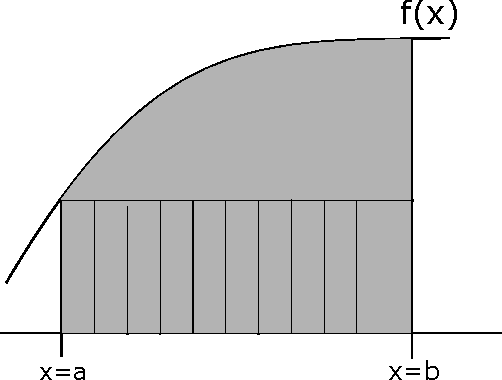
\includegraphics[width=0.5\textwidth]{RectangleRule.pdf}
    \caption{Rectangle Rule}
    \label{fig:1}
\end{figure}
\subsection{Mid-point Rule}
\textbf{If} $x_0 = \frac{a+b}{2}$, then the approximation would be,
\begin{equation}
    I(f) \approx M = (b-a) f\left(\frac{a+b}{2}\right)
\end{equation}
is known as the \textbf{mid-point rule}.
\begin{figure}[h!]
    \centering
    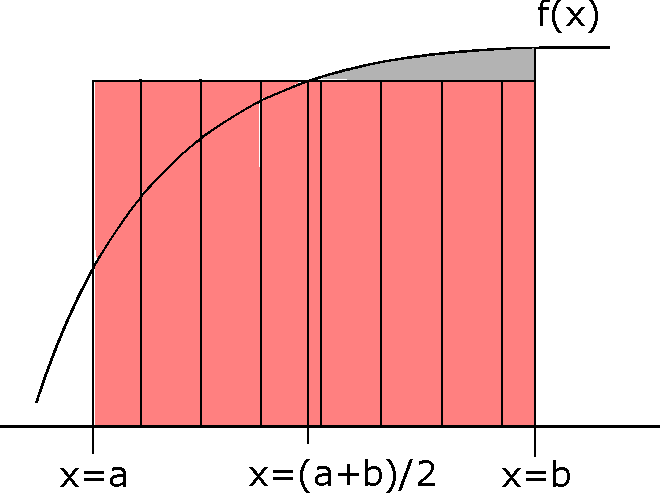
\includegraphics[width = 0.5\textwidth]{MidPointRule.pdf}
    \caption{Mid-Point Rule}
    \label{fig:2}
\end{figure}
\subsection{Trapezoidal Rule}
Let $k=1$. Then
\[f(x) \approx f(x_0) + f[x_0,x_1](x-x_0)\]
\textbf{Choosing $x_0 = a$ and $x_1 = b$} to have,
\[ I(p_1) = \int_a^b \left( f(a) + f[a,b](x-a) \right) dx\]
or,
\begin{equation}
    I(f)\approx T = \frac{1}{2}(b-a)[f(a)+f(b)]
\end{equation}
which yields the \textbf{trapezoidal rule}.
\begin{figure}
    \centering
    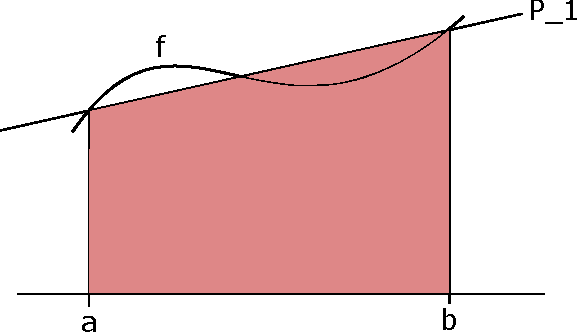
\includegraphics[width=0.5\textwidth]{TrapezoidalRule.pdf}
    \caption{Trapezoidal Rule}
    \label{fig:3}
\end{figure}
\subsection{Simpson's Rule}
Let $k=2$. Then
\[f(x) \approx p_2(x)\]
\textbf{If we choose $x_0 = a$, $x_1 = \frac{a+b}{2}$ and $x_2 = b$}, then the interpolating polynomial $p_2(x)$ is in the form,
\[p_2(x) = f(a) + f[a,b](x-a) + f\left[a,b,\frac{a+b}{2}\right](x-a)(x-b)\]
Then, the approximate integral would be,
\begin{equation}
    \begin{split}
        I(f) \approx I(p_2) &= f(a)(b-a) + f[a,b]\frac{(b-a)^2}{2} + f\left[ a,b,\frac{a+b}{2} \right]\int_a^b(x-a)(x-b)dx\\
        &=f(a)(b-a) + f[a,b]\frac{(b-a)^2}{2} + f\left[ a,b,\frac{a+b}{2} \right]\frac{(b-a)^3}{6}\\
        &= (b-a)\left\{ f(a) + \frac{f(b) -f(a)}{2} -2 \frac{\left( f(b) - f\left( \frac{a+b}{2} \right) + f(a)\right)}{6}\right\}\\
        &= \frac{b-a}{6} \left\{ f(a) + 4f\left(\frac{a+b}{2} \right) + f(b) \right\}
    \end{split}
\end{equation}
Thus, the quadrature formula becomes,
\begin{equation}
    I(f) \approx S = \frac{b-a}{6} \left\{ f(a) + 4f\left( \frac{a+b}{2}\right) + f(b) \right\}
\end{equation}
which is called the \textbf{Simpson's Rule}.
\begin{figure}
    \centering
    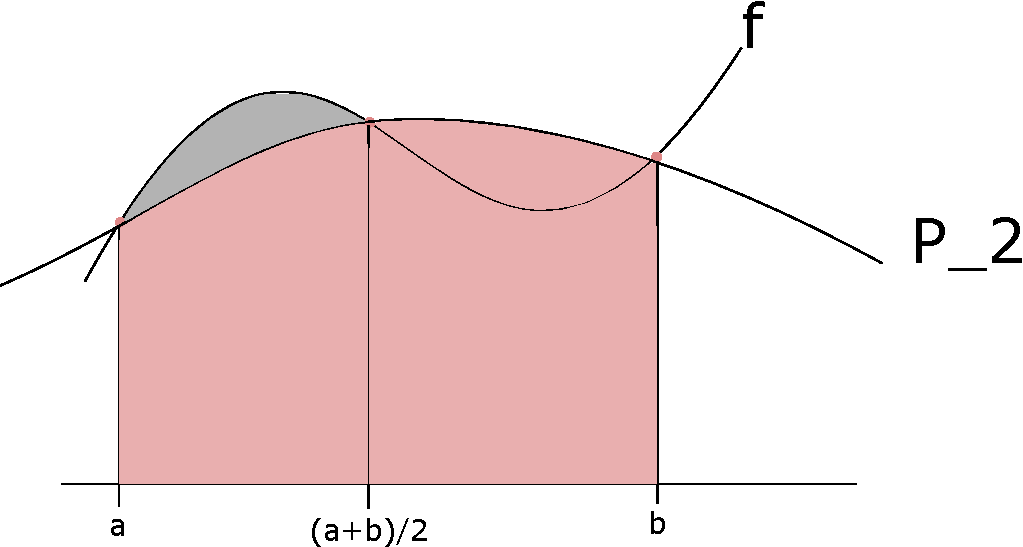
\includegraphics[width = 0.5\textwidth]{SimpsonRule.pdf}
    \caption{Simpson's Rule}
    \label{fig:4}
\end{figure}
\subsection{Corrected Trapezoidal Rule}
Suppose we have $k=3$. Then, as usual,
\[f(x) \approx p_3(x)\]
\textbf{Choosing $x_0 = x_1 = a$ and $x_2 = x_3 = b$}, we notice that,
\begin{equation*}
    p_3(x) = f(a) + f[a,a](x-a) + f[a,a,b](x-a)^2 + f[a,a,b,b](x-a)^2(x-b)
    \end{equation*}
Now, integrating $p_3(x)$ leads to the following approximation,
\begin{equation}
    \begin{split}
        I(f) \approx I(p_3) = \int_a^bp_3(x) dx &= \frac{b-a}{2}[f(a) + f(b)] + \frac{(b-a)^2}{12}[f^\prime(a) - f^\prime(b)]
    \end{split}
\end{equation}
which is known as \textbf{corrected trapezoidal rule}.  
\begin{figure}[h!]
    \centering
    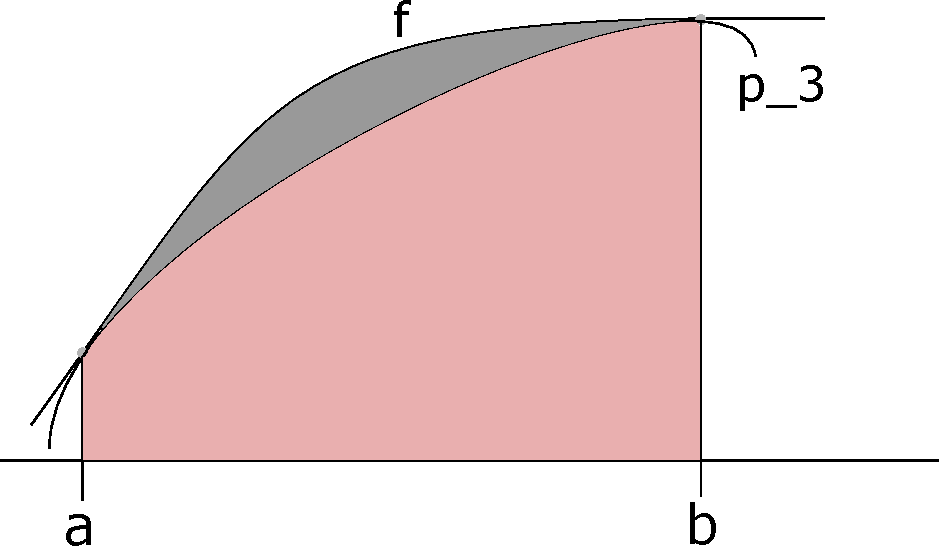
\includegraphics[width = 0.5\textwidth]{CorrectedTrapezoidalRule.pdf}
    \caption{Corrected Trapezoidal Rule}
    \label{fig:5}
\end{figure}
\section{Error Analysis}
So far, we've seen the various methods to approximate the integral of a function $f$ by approximating it via Newton's Interpolating method. A very obvious question that arises in mind after seeing all the methods is \textbf{the amount of error we are incurring in approximating the integral via Newton's interpolating polynomial}. Note that if we are able to quantify the error, then it would be much easier to judge which rule is most suitable for a given function $f$. Hence we now do exactly that, i.e. quantify the error.
\nll
By Newton's divided difference, we can write,
\[ f(x) = p_k(x) + f[x_0,\dots,x_k,x]\psi_k(x) \]
where $\psi_k(x) = \prod_{j=0}^k(x-x_j)$. The error $E(f)$ is given by,
\begin{equation*}
    \begin{split}
        E(f) = I(f) - I(p_k) &= \int_a^b f[x_0,\dots,x_k,x]\psi_k(x) dx
    \end{split}
\end{equation*}
$\boxed{\star}$ \textbf{If $\psi_k(x)$ is only of one sign in interval $[a,b]$}, then by Mean Value Theorem
\[ \int_a^b f[x_0,\dots,x_k,x] \psi_k(x) dx = f[x_0,\dots,x_k,\xi] \int_a^b \psi_k(x)dx \]
for some $\xi \in (a,b)$. If $f(x) \in C^{k+1}(a,b)$, then it follows that the error by Theorem 8.9 is,
\begin{equation}
    \boxed{E(f) = \frac{1}{(k+1)!} f^{(k+1)}(\eta) \int_a^b\psi_k(x)dx \;\;\text{for some}\;\;\eta \in(a,b)}
\end{equation}
$\boxed{\star}$ \textbf{Even if $\psi_k(x)$ is not of one sign, certain simplifications in the error $E(f)$ are possible.} One particular desirable instance of this kind occurs when,
\begin{equation}
    \int_a^b \psi_k(x)dx = 0
\end{equation}
For this case, we can use the identity,
\begin{equation}
    f[x_0,\dots,x_k,x] = f[x_0,\dots,x_k,x_{k+1}] + f[x_0,\dots,x_{k+1},x](x-x_{k+1})
\end{equation}
which is true for arbitrary $x_{k+1}$. Then the error $E(f)$ becomes
\begin{equation}
    \begin{split}
        E(f) &= \int_a^bf[x_0,\dots,x_{k+1}]\psi_k(x)dx + \int_a^b f[x_0,\dots,x_{k+1},x](x-x_{k+1})dx\\
        &= \int_a^b f[x_0,\dots,x_{k+1},x] \psi_{k+1}(x)dx
    \end{split}
\end{equation}
where $\psi_{k+1}(x)dx = (x-x_{k+1})\psi_k(x)$.
\nll
Now \textbf{choose} $x_{k+1}$ in such a way that \textbf{$\psi_{k+1}(x)= (x-x_{k+1})\psi_k(x)$ is of one sign on $(a,b)$}. Thus, if $f(x) \in C^{k+2}(a,b)$ then,
\begin{equation}
    \boxed{E(f) = \frac{1}{(k+2)!} f^{(k+2)}(\eta)\int_a^b\psi_{k+1}(x)dx\;\;\text{for some}\;\; \eta \in (a,b)}
\end{equation}
\subsection{Error in Rectangle Rule}
In this case, we only have one point $x_0 = a$, hence,
\[\psi_0(x) = (x-a)\]
Thus, the error becomes,
\[E_R = E(f) = \int_a^b f[x_0,x](x-a)\]
$\boxed{\star}$ Now since \tit{$\psi_0(x)$ is of one sign in $(a,b)$}, hence we would use Eq. 10.10 to get,
\begin{equation}
    E_R = f^\prime(\eta) \int_a^b (x-a)dx = \boxed{\frac{f^\prime(\eta)(b-a)^2}{2}}
\end{equation}
\subsection{Error in Mid-Point Rule}
In this case, we still have only one point, however, that point is the mid-point of the interval $(a,b)$, thus $x_0 = \frac{a+b}{2}$.
\nll
Note that in this case, 
\[\psi_0(x) = (x-\frac{a+b}{2})\]
which is of NOT the same sign for $x\in (a,b)$. But note that,
\[\int_a^b \psi_0(x) dx = \int_a^b \left( x-\frac{a+b}{2}\right)dx = 0\]
Thus we can now simply use the second method discussed above.
\nll
For that, if we introduce another point $x_1 = \frac{a+b}{2}$, then 
\[\psi_1(x) = (x-x_1)\psi_0(x) = (x-\frac{a+b}{2})^2\] 
\textbf{is of one sign}. Thus, by Eq. 10.14, we get,
\begin{equation}
    \boxed{E_M =\frac{f^{\prime\prime}(\eta)(b-a)^3}{24} \;\;\text{for some}\;\; \eta \in (a,b)}
\end{equation}
\subsection{Error in Trapezoidal Rule}
In this case, we have two points $x_0 = a$ and $x_1 = b$. Therefore, 
\[\psi_1(x) = (x-a)(x-b)\]
As $\psi_1(x)$ is of one sign on $(a,b)$, thus, we can simply use the Eq. 10.10 so that the error in Trapezoidal Rule $E_T$ becomes,
\begin{equation}
    \boxed{E_T = \frac{f^{\prime\prime}(\eta)}{2} \int_a^b (x-a)(x-b)dx = \frac{f^{\prime\prime}(\eta)(b-a)^3}{12} \;\;\text{for some}\;\; \eta \in (a,b)}
\end{equation}
\subsection{Error in Simpson's Rule}
In this case, we have 3 points as $x_0 = a$, $x_1 = \frac{a+b}{2}$ and $x_2 = b$. Thus, the $\psi_2(x)$ is,
\[\psi_2(x) = (x-a)(x-b)\left( x-\frac{a+b}{2} \right)\]
Now note that in $(a,b)$, the sign of $\psi_2(x)$ is NOT same. But still, note that,
\[\int_a^b \psi_2(x)dx = \int_a^b (x-a)(x-b)\left( x-\frac{a+b}{2} \right) dx = 0\]
Hence we can \textbf{use the second method} in this case! For that all, we need to find is another point $x_3$ such that $\psi_3(x)$ \textbf{should be of same sign in $(a,b)$}. 
\nll
For this, first see that
\[\psi_4(x) = (x-a)(x-b)(x-x_3)\left(x-\frac{a+b}{2}\right)\]
and note that it can be of same sign on $(a,b)$ only when $x_3 = \frac{a+b}{2}$. Thus, the error for Simpson's Rule can now can be written with the help of Eq. 10.14 as,
\begin{equation}
    \begin{split}
        E_S &= \frac{f^{(4)}(\eta)}{24} \int_a^b (x-a)(x-b)\left(x-\frac{a+b}{2}\right)^2dx\\
        &= \frac{f^{(4)}(\eta)}{24}\times \frac{-4}{15}\left( \frac{b-a}{2} \right)^5\\
        &\boxed{= -\frac{f^{(4)}(\eta)}{90}\left( \frac{b-a}{2} \right)^5\;\;,\;\eta \in (a,b)}.
    \end{split}
\end{equation}
\subsection{Error in Corrected Trapezoidal Rule}
We have three points here, $x_0 = x_1 = a$ and $x_2 = x_3 = b$. Now note that,
\[ \psi_3(x) = (x-a)^2(x-b)^2 \]
is of one sign on (a,b) and hence we can simply use Eq. 10.10 to get the error $E_{CT}$ as,
\begin{equation}
\begin{split}
    E_{CT} &= \frac{{f^{(4)} (\eta)}}{4!} \int_a^b (x-a)^2(x-b)^2 dx\\
    &= \boxed{\frac{f^{(4)}(\eta) (b-a)^5}{720}\;\eta \in (a,b)}
    \end{split}
\end{equation}
\section{Composite Methods}
Let's take a look at Figure \ref{fig:1}. The boxed one represents the area actual approximation and the whole grey region is the actual value of $\int_a^bf(x)dx$. We can clearly see intuitively that this would contain heavy amount of error. This was also confirmed by error analysis and Eq. 10.15. It grows quadratically with the size of interval $(a,b)$. 
\nll
One way to overcome this might be to use different length rectangles in each subinterval after dividing the original interval. This would bring us somewhat closer to the Darboux's definition of Riemann integral. Thus, our aim now is to find a scheme to fit the length of rectangle which we should make dependent on the subinterval of $(a,b)$. This is called composite rule where we use the previously discussed rules in the context of each subinterval of $(a,b)$ instead of using it on whole of $(a,b)$ at once.
\subsection{Composite Rectangle Rule}
Divide $[a,b]$ into $N$ subintervals to get,
\[a = x_0 < x_1 < x_2 < \dots < x_N = b\]
where $x_i = a+ih\;,\;\;i=0,\dots,N$ with \textbf{uniform step-size} $h = \frac{b-a}{N}$.
\nll
Set,
\[f_i = f(x_i) = f(a+ih)\;,\;\;i=0,\dots,N\]
and,
\[f_{i-\frac{1}{2}} = f(x_i - \frac{h}{2}).\]
Now, simply apply the \textbf{Rectangular Rule on each subinterval} to get,
\begin{equation*}
\begin{split}
    \int_{x_{i-1}}^{x_i}f(x)dx &= (x_i - x_{i-1})f(x_{i-1}) +  \underbrace{\frac{f^\prime(\eta_i)(x_i - x_{i-1})^2}{2}}_{\text{Error Term (Eq. 10.15)}}\\
    &= hf(x_{i-1}) + \frac{f^{\prime}(\eta_i)h^2}{2}
\end{split}
\end{equation*}
Summing from $i=1$ to $i=N$, we obtain,
\begin{equation}
   \boxed{ I(f) = \int_a^bf(x)dx = h\sum_{i=1}^N f_{i-1} + \sum_{i=1}^N \frac{f^\prime(\eta_i)h^2}{2} = R_N + E_N^R}
\end{equation}
where $\eta_i \in (x_{i-1},x_i)$ and $R_N$ is called the \textbf{Composite Rectangle Rule}.
\nll
Note that if $f^\prime(x)$ is continuous, then we can write,
\[\sum_{i=1}^N \frac{f^\prime(\eta_i)h^2}{N} = f^\prime(\eta) \sum_{i=1}^N \frac{h^2}{2} = \frac{f^\prime(\eta)Nh^2}{2} \]
with $Nh = b-a$, it becomes,
\begin{equation}
    E_N^R = \frac{f^\prime(\eta)(b-a)h}{2} \;\;\text{for some}\;\;\eta \in (a,b)
\end{equation}
\subsection{Composite Mid-Point Rule}
Continuing as in the previous subsection for the rectangle rule, we can do the same now for the Mid-Point rule,
\begin{equation}
\begin{split}
   I(f) \int_a^b f(x)dx &= \sum_{i=1}^N \int_{x_{i-1}}^{x_i} f(x)dx\\
    &\approx h \sum_{i=1}^N f(x_{i-\frac{1}{2}}) \\
    &= \boxed{h\sum_{i=1}^Nf_{i-\frac{1}{2}}}
\end{split}
\end{equation}
where the error can be similarly found to be,
\begin{equation}
        E_N^M = \frac{f^{\prime\prime}(\xi)(b-a)h^2}{24}
\end{equation}
\subsection{Composite Trapezoid Rule}
Using Eq. 10.6,
\begin{equation}
    \begin{split}
        I(f) = \int_a^bf(x)dx &= \sum_{i=1}^N \int_{x_{i-1}}^{x_i}f(x)dx\\
        &\approx \frac{h}{2} \sum_{i=1}^N[f(x_{i-1}) + f(x_i)]\\
       T_N &= \boxed{\frac{h}{2} \left[ f_0 + 2\sum_{i=1}^{N-1}f_i + f_N \right]}
    \end{split}
\end{equation}
and the error $E^T_N$ follows from Eq. 10.17,
\begin{equation}
    E_N^T = -\frac{f^{\prime\prime}(\eta)(b-a)h^2}{12}
\end{equation}
\subsection{Composite Simpson's Rule}
As usual, letting $a = x_{i-1}$, $b=x_i$ and $x_i - x_{i-1} = h$, apply Simpson's Rule over a single subinterval $(x_{i-1},x_i)$ in conjunction with result in Eq. 10.7 to obtain,
\begin{equation*}
\begin{split}
    \int_{x_{i-1}}^{x_i} f(x)dx &= \frac{h}{6} \left[ f_{i-1} + 4f_{i-\frac{1}{2}} + f_i \right] - \frac{f^{(4)}(\eta_i)\left( \frac{h}{2}\right)^5}{90}\;,\;\;x_{i-1} < \eta_i < x_i
\end{split}
\end{equation*}
Now simply summing over all subintervals $i=1,\dots,N$ to obtain,
\begin{equation}
    \begin{split}
        I(f) &= \sum_{i=1}^N \int_{x_{i-1}}^{x_i} f(x)dx = \frac{h}{6} \sum_{i=1}^N \left[ f_{i-1} + 4f_{i-\frac{1}{2}} + f_i \right] - \sum_{i=1}^N\frac{f^{(4)}(\eta_i)\left( \frac{h}{2}\right)^5}{90}\\
        &= S_N + E_N^S
    \end{split}
\end{equation}
The composite Simpson approximation $S_N$ can be simplified to have,
\begin{equation}
    \boxed{S_N = \frac{h}{6}\left[ f_0 + f_N + 2\sum_{i=1}^{N-1}f_i + 4\sum_{i=1}^N f_{i-\frac{1}{2}} \right]}
\end{equation}
with the error term $E_N^S$ being,
\begin{equation}
    E_N^S = \frac{f^{(4)}(\xi)(b-a)\left(\frac{h}{2}\right)^4}{180} \;\; a<\xi<b
\end{equation}
\subsection{Composite Corrected Trapezoidal Rule}
Following from Eq. 10.9,
\begin{equation}
\begin{split}
    I(f) &= \sum_{i=1}^N\int_{x_{i-1}}^{x_{i}} f(x)dx = \int_{x_0}^{x_1} f(x)dx + \dots + \int_{x_{N-1}}^{x_N} f(x)dx\\
    &\approx \frac{h}{2}[f(x_0) + f(x_1)] + \frac{h^2}{12} [f^\prime(x_0) - f^\prime(x_1)]\\
    &+ \dots + \frac{h}{2}[f(x_{N-1}) + f(x_N)] + \frac{h^2}{12} [f^\prime(x_{N-1}) - f^\prime(x_N)]
\end{split}
\end{equation}
Now note that all the interior derivatives form a \tit{telescopic series}, thus cancelling each other except the first and the last terms. Thus, the \textbf{Composite Corrected Trapezoidal Rule} is,
\begin{equation}
    \begin{split}
    \boxed{I(f)\approx CT_N = \frac{h}{2}\left( f_0 + f_N + 2\sum_{i=1}^{N-1} f_i \right) + \frac{h^2}{12}[f^\prime(a) - f^\prime(b)]  }
    \end{split}
\end{equation}
and the error term $E_N^{CT}$ can be seen from Eq. 10.19 to be,
\begin{equation}
    E_N^{CT} = \frac{f^{(4)}(\eta)(b-a)(h)^4}{720}\;\;,a<\eta<b
\end{equation}
\section{Gauss Quadrature Rule}
Quadrature is a historic word which means \textit{the area} under a curve, thus, an integral. In fact, we have seen three quadrature rules already, where any quadrature rule has the form,
\begin{equation}
    I(f) \approx A_0 f(x_0) + A_1f(x_1) + \dots + A_k f(x_k)
\end{equation}
with \textbf{nodes} $x_0,\dots,x_k$ and \textbf{weights} $A_0,\dots,A_k$.
\nll
Note that this encompasses all the following rules,
\begin{equation*}
    \begin{split}
    I(f) &\approx (b-a)f(x)\;\;\text{(Rectangle Rule)}\\
    I(f) &\approx \frac{(b-a)}{2} [f(a) + f(b)]\;\;\text{(Trapezoidal Rule)}\\
    I(f) &\approx \frac{(b-a)}{6} \left[ f(a) + 4f\left( \frac{a+b}{2} \right)  + f(b)\right]\;\;\text{(Simpson's Rule)}
    \end{split}
\end{equation*}
$\boxed{\star}$ Now note that there is no apparent freedom in choosing the nodes $x_0,x_1,\dots,x_k$. The difficulty with the Composite Rules is that the nodes $x_i$ \textbf{must be evenly spread}.
\nll
Thus a natural question to ask is \textit{\textbf{whether it is possible to make a rule for polynomial of degree $\le 2k+1$ by choosing the nodes appropriately?}}
\nll
To discuss the Gaussian Rules in the more general context, we write the integral as
\[\int_a^b f(x)dx = \int_a^b w(x)g(x)dx\]
where the \textbf{weight function} $w(x)$ is assumed to be \tit{non-negative} and \tit{integrable} on $[a,b]$ and,
\[ g(x) = \frac{f(x)}{w(x)} \]
Consider approximating the weighted integral,
\begin{equation*}
\begin{split}
    I(g) &= \int_a^b g(x)w(x) dx\\
    &\approx A_0g(x_0) + A_1g(x_1) + \dots + A_kg(x_k)\\
    &= \sum_{j=0}^k A_j g(x_j) = I_k(g)
\end{split}
\end{equation*}
We can clearly see in the above equations that the nodes $x_j$ and weights $A_j$ are to be chosen so that $I_k(g)$ equals $I(g)$ exactly for polynomials $g(x)$ of \textit{as higher degree as possible}. This is indeed the basic idea behind the \textbf{Gaussian Rule}.
\subsection{Special case when $w(x) = 1$ and $\int_{-1}^1 g(x) dx \approx \sum_{j=0}^k A_j g(x_j)$}
In this case, we define the \textbf{Error} as,
\begin{equation}
\begin{split}
   \boxed{ E_k(g) = \int_{-1}^1 g(x)dx - \sum_{j=0}^k A_j g(x_j)}
\end{split}
\end{equation}
Now the task is to \textbf{determine the weights $A_j$ and nodes $x_j$ to make the error 0}, i.e.
\begin{equation}
    E_k(g) = 0
\end{equation}
\textbf{for as high a degree polynomial $g(x)$ as possible}.
\nll
Note that,
\begin{equation}
    E_k(a_0 + a_1 x  + \dots + a_n x^m) = a_0E_k(1) + a_1E_k(x) + \dots + a_mE_k(x^m)
\end{equation}
Also, note that, 
\begin{equation}
\begin{split}
    &E_k(g) = 0 \;\;\text{for every polynomial of degree}\;\le m \\
    \iff& \;\;E_k(x^i) = 0,\;i=0,1,2,\dots,m.
    \end{split}
\end{equation}
Hence, to show that $E_k(g) =0 $ is equivalent to showing that each $E_k(x^i) = 0$ for all $i=0,1,\dots,m$. We now use exactly this equivalence. 
\subsubsection{$\boxed{\text{For}\; k=0}$}
We have,
\[ \int_{-1}^1 g(x)dx \approx A_0g(x_0) \]
Due to the conditions, \textbf{we require $E_k(1)= 0$ and $E_k(x) = 0$}.
\begin{equation}
\begin{split}
    E_k(1) = 0 &\implies \int_{-1}^1 dx - A_0 \implies A_0 = 2\\
    E_k(x) = 0 &\implies \int_{-1}^1xdx - A_0x_0 \implies x_0 = 0
\end{split}
\end{equation}
Therefore, we would be lead to the following formula,
\begin{equation*}
    \boxed{\int_{-1}^1 g(x)dx \approx 2g(0)}
\end{equation*}
which is the \textbf{Mid-Point Rule!}
\subsubsection{$\boxed{\text{For} \;\ k=1}$}
We have,
\[ \int_{-1}^1 g(x) dx \approx A_0g(x_0) + A_1g(x_1) \]
Note there are \textbf{four unknown parameters} to be determined.
\nll
Thus we require,
\begin{equation}
\begin{split}
    E_k(1) = 0 &\implies \int_{-1}^1dx - A_0-A_1 = 0 \implies A_0 + A_1 = 2\\
    E_k(x) = 0 &\implies \int_{-1}^1xdx - (A_0x_0 + A_1x_1) = 0 \implies A_0x_0 + A_1x_1 = 0\\
    E_k(x^2) = 0 &\implies \int_{-1}^1 x^2 dx - (A_0x_0^2 + A_1x_1^2) = 0 \implies A_0x_0^2 + A_1x_1^2 = \frac{2}{3}\\
    E_k(x^3) = 0 &\implies \int_{-1}^1 x^3dx - (A_0x_0^3 + A_1x_1^3) = 0 \implies A_0x_0^3 + A_1x_1^3 = 0
\end{split}
\end{equation}
On solving, we get,
\begin{equation*}
\begin{split}
    A_0 &= 1\\
    A_1 &= 1\\
    x_0 &= \frac{1}{\sqrt{3}}\\
    x_1 &= -\frac{1}{\sqrt{3}}
\end{split}
\end{equation*}
This leads to the formula,
\begin{equation*}
    \boxed{\int_{-1}^1 g(x)dx \approx g\left( \frac{1}{\sqrt{3}}\right) + g\left(-\frac{1}{\sqrt{3}}\right)}
\end{equation*}
which has a degree of precision 3.
\subsubsection{$\boxed{\text{For a general} \;k}$}
There are $2k+2$ parameters, weights $\left\{ w_i \right\}_{i=0}^k$ and nodes $\left\{ x_i \right\}_{i=0}^k$, to be determined.
\nll
The equations to be solved are,
\begin{equation}
    E_k(x^i) = 0\;,\;\;i=0,1,\dots,2k+1
\end{equation}
This leads to the following set of equations:
\begin{equation}
\begin{split}
   \boxed{\boxed{ \sum_{j=0}^k A_jx_j^i = \begin{cases} 0 \;\;& i=1,3,\dots,2k+1.\\
    \frac{2}{i+1} \;\;& i=0,2,\dots,2k.
    \end{cases}}}
\end{split}
\end{equation}
However, note that the equations in Eq. 10.40 are non-linear equations and their solvability is not at all obvious. For that, we \textbf{may} have the following alternative
\subsection{An Alternate Approach through Newton's Interpolation}
First, choose $x_0,\dots, x_k$ in $(a,b)$ and write the Newton's Interpolating Polynomial (Theorem 8,8),
\[ g(x) = p_k(x) + g[x_0,x_1,\dots,x_k,x]\psi_k(x) \]
where $p_k(x)$ is the polynomial of degree $\le k$ which interpolates $g(x)$ at $x_0,\dots,x_k$ with,
\[\psi_k(x) = (x-x_0)\dots(x-x_k)\]
This now leads to, after integrating both sides,
\begin{equation}
    I(g) = I(p_k) + \underbrace{\int_a^bg[x_0,\dots,x_k,x]\psi_k(x)w(x)dx}_{\text{Error Term}}
\end{equation}
Now, if we write $p_k(x)$ in Lagrange form (Eq. 8.3) then,
\[ p_k(x) = g(x_0)L_0(x) + g(x_1)L_1(x) + \dots + g(x_k)L_k(x) \]
with,
\[L_i(x) = \prod_{j=0,i\neq j}^k\frac{(x-x_j)}{(x_i-x_j)}\;,\;\;i=0,\dots,k\]
Thus, expanding $I(p_k)$ in Eq. 10.41 now yields,
\begin{equation*}
\begin{split}
    I(p_k) &= \int_a^b p_k(x)w(x)dx\\
    &= g(x_0)\int_a^b L_0(x)w(x)dx + \dots + g(x_k)\int_a^bL_k(x)w(x)dx
\end{split}
\end{equation*}
Hence we can write $I(p_k)$ simply as,
\begin{equation}
    I(p_k) =A_0g(x_0) + A_1g(x_1) + \dots + A_kg(x_k)
\end{equation}
where coefficients $A_i$ are simply,
\begin{equation}
    A_i = \int_a^b L_i(x)w(x)dx\;,\;\;i=0,\dots,k 
\end{equation}
Now, for the error term, \textbf{using the property of orthogonal polynomials}, for many $w(x)$, \textbf{we can find a polynomial $P_{k+1}(x)$} such that,
\begin{equation}
    \int_a^b P_{k+1} (x)q(x)w(x)dx = 0
\end{equation}
for all polynomial $q(x)$ of degree $\le k$. Moreover, since $P_{k+1}(x)$ is a polynomial, thus,
\[P_{k+1}(x) = \alpha_{k+1}(x-\xi_0)(x-\xi_1)\dots(x-\xi_k)\]
where $\xi_0,\dots,\xi_k$ are the $k+1$ distinct points in the interval $(a,b)$ at which $P_{k+1}$ vanishes.
\nll
Now, \textbf{simply set,}
\begin{equation}
    x_j = \xi_j\;,\;\;j=0,\dots,k
\end{equation}
to get 
\[I(f) = I(p_k)\]
as the error term becomes zero. But the difficulty being finding the right $P_{k+1}$'s.
\nll
$\boxed{\star}$ Hence, if we choose the points $x_0,\dots,x_k$ as the zeros of the polynomial $P_{k+1}(x)$ of degree $k+1$, which is orthogonal to the weight function $w(x)$ over $(a,b)$ to any polynomial of degree $\le k$, and if the coefficients $A_i$ for $i=0,\dots,k$ are chosen in accordance with Eq. 10.43, then \textbf{the resulting Gaussian Quadrature Formula will then be EXACT for all polynomials of degree $\le 2k+1$}.
\nll
But we see that determining $P_{k+1}(x)$ is not at all obvious. One thing we can do, however, is to choose the orthogonal polynomials $P_{k+1}$ to be \textbf{Legendre Polynomials}! But the Legendre polynomials are only defined over $(-1,1)$. Thus, one needs to transform original integral $\int_a^bf(x)dx$ over the limits $-1$ and $1$ to write $\int_{-1}^1g(\tau) d\tau$. This can be done using the following change of variable,
\[x = \frac{(b-a)t + (b+a)}{2}\]
Now, we can use the argument above to, for any $k$, construct the Orthogonal Legendre Polynomials, find it's roots $\xi_i$, subsequently exactly calculate the integral by Eq. 10.42, 10.43 and $x_i = \xi_i$.
\nll
Refer to Example in Lecture 20 for more rigidity.
\chapter{Numerical Solutions to IVPs for ODEs : One-Step Method}
We first consider the first-order ordinary differential equations as we can use the same idea to extend these ideas to higher order ODEs as they can be written as a system of first order ODEs.
\nll
Consider a first-order IVP of the form
\begin{equation}
\label{11.1}
    y^\d = f(x,y)\;,\;\;y(x_0) = y_0
\end{equation}
where the function $f$ may be linear or non-linear.
\nll
Clearly, before jumping into the numerical techniques, we must first make sure concretely that the question we are trying to solve indeed has a solution and that the solution is unique. To that extent, for IVP in Eq. \ref{11.1}, we have the following theorem,
\nll
\theor{13} : \textbf{(Unique Solution of Eq. \ref{11.1})} \tit{If $f(x,y)$ is continuous in a rectangle
\[R = \{ (x,y) \;:\; \abs*{x-x_0} \le a\;,\;\;\abs*{y-y_0}\le b \}\]
satisfies a Lipschitz condition in the second variable
\[\abs*{f(x,y_1) - f(x,y_2)} \le L\abs*{y_1-y_2}\;\;\forall (x,y_1),(x,y_2) \in \mathbb{R}^2\]
Then the IVP in Eq. \ref{11.1} has \textbf{a unique solution} in the interval $\abs*{x-x_0}\le \alpha$ where,
\[\alpha = \min\left\{ a,\frac{b}{M} \right\} \;\;\text{and}\;\;M=\underset{R}{\max}\abs*{f(x,y)}\]
 }
\section{Taylor-Series Method}
Note that we can expand the $y(x)$ into it's Taylor Series to get,
\begin{equation*}
\begin{split}
    y(x) &= y(x_0) + (x-x_0)y^\d(x_0) + \frac{(x-x_0)^2}{2!} y^{\d\d}(x_0) + \dots\\
    &= y_0 + hy^\d(x_0) + \frac{h^2}{2!} y^{\d\d}(x_0)+ \dots
\end{split}
\end{equation*}
where $x-x_0 = h$. \textbf{If $f$ is sufficiently differentiable with respect to $x$ and $y$}, we can compute,
\begin{equation*}
\begin{split}
    y^\d &= f(x,y)\\
    y^{\d\d} &= f^\d = f_x + f_y y^\d = f_x + f_yf\\
    y^{\d\d\d} &= f^{\d\d} = f_{xx} + f_{xy}f + f_{yx}f + f_{yy}f^2 + f_yf_x + f_y^2f\\
    &\text{and so on} \dots
\end{split}
\end{equation*}
Now let $y_n$ \textbf{be approximations to the true solutions} $y(x_n)$ at the points $x_n = x_0 + nh\;,\;\;n=0,1,2,\dots$. That is,
\begin{equation*}
    y_n \approx y(x_n)
\end{equation*}
We thus arrive at the \textit{Taylor's Algorithm of Order $k$.}
\subsection{Taylor's Algorithm of Order $k$}
\algo : To find an approximate solution of the IVP
\[y^\d = f(x,y)\;,\;\;y(x_0) = y_0\]
over an interval $[a,b]$.
\begin{enumerate}
    \item[\textit{Step 1 : }]{Choose a step size $h = \frac{b-a}{N}$. Set,
    \[x_n = x_0 + nh\;,\;\;n = 0,1,\dots,N\]
    }
    \item[\tit{Step 2 : }]{Generate approximations $y_n$ to $y(x_n)$ from the recursion
    \[y_{n+1} = y_n + hT_k(x_n,y_n)\;,\;\;n=0,1,\dots,N-1\]
    where $T_k$ is,
    \[T_k(x,y) = f(x,y) + \frac{h}{2!}f^\d(x,y) + \dots\frac{h^{k-1}}{k!}f^{(k-1)}(x,y)\;,\;\;k=1,2,\dots\]
    Here, $f^{(j)}$ denotes the $j^{th}$ derivative of the function $f(x,y(x))$ with respect to $x$.
    \nll
    So we are basically truncating the Taylor series to $k^{th}$ order and take the $h$ common out from them as $y^\d = f$.
    \nll
    Note that we calculate $y$ at $x = x_{n+1}$ by using only the information about $y$ and it's derivatives at the previous step $x = x_n$. Such a method is thus called \textbf{One-Step/Single-Step Method}.}
    
\end{enumerate}
\subsubsection{Error in Taylor's Algorithm}
Taylor's Theorem with remainder term shows the local error of Taylor's Algorithm of order $k$ can be written as,
\begin{equation}
    E = \frac{h^{k+1}}{(k+1)!} f^{(k)}(\xi , y(\xi)) = \frac{h^{k+1}}{(k+1)!} y^{(k+1)}(\xi) \;,\;\;x_n < \xi < x_n + h
\end{equation}
The Taylor algorithm is said to be of \textbf{order $k$ if the local error $E$ is $O(h^{(k+1)})$}.
\section{Euler's Method}
Setting $k=1$ (Taylor's Algorithm of Order 1), we obtain,
\begin{equation}
    y_{n+1} = y_n + hf(x_n,y_n)
\end{equation}
which is known as \textbf{Euler's Method}. Note that the $x_n$ is still calculated as per the Taylor's Algorithm. The \textbf{Local Error} is simply
\begin{equation}
    E = \frac{h^2}{2}y^{\d\d}(\xi)
\end{equation}
\begin{figure}[h!]
    \centering
    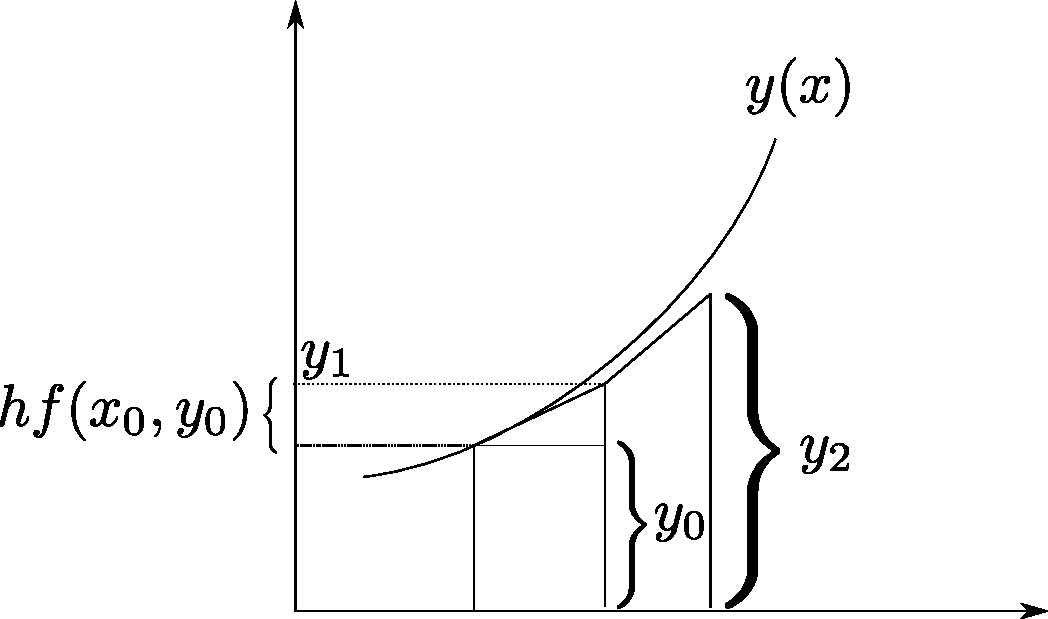
\includegraphics[width=0.5\textwidth]{EulerMethodODE.pdf}
    \caption{Geometric Interpretation of Euler's Method.}
    \label{fig:EulerMethodODE}
\end{figure}
\newpage
\subsubsection{Error in Euler's Method}
\theor{14}  : (\textbf{Error Estimate}) \tit{Let $y_n$ be the approximate solution of \[y^\prime = f(x,y)\;,\;\;y(x_0) = y_0\]
as generated by Euler's Method. If $y^{\d\d} \in C([x_0,b])$ and
\[\abs*{f_y(x,y)} < L\;,\;\;\abs*{y^{\d\d}(x)} < M\;,x \in [x_0,b]\]
for fixed positive constants $L$ and $M$, then, the \textbf{error $e_n = y(x_n) - y_n$ of Euler's method at a point $x_n = x_0 + nh$ is bounded} as follows,
\[ \abs{e_n} \le \frac{hM}{2L} \left[ e^{(x_n-x_0)L} - 1 \right] \]
}
This theorem shows that the error is $O(h)$ and $e_n \to 0$ as $h\to 0$.
\nll
Refer to Lecture 21 for a small example.
\section{Runge-Kutta Method}
We previously saw that in Taylor's Algorithm of order $k$ and that in Euler's Method, one needs higher order derivatives of a function. But we definitely don't have that information with us. Moreover, the approximations done by such methods only produce results with low error when $h$ is low enough. Thus, we try to look at the methods which only require function calculations instead of requiring to calculate an explicit form of other functions.
\nll
To that extent, the Runge-Kutta Method plays a major step. In this method, we seek a formula of the form,
\begin{equation}
\label{11.5}
\begin{split}
    y_{n+1} &= y_n + ak_1 + bk_2\\
k_1 &= hf(x_n,y_n)\;,\;\; k_2 = hf(x_n + \alpha h,y_n + \beta k_1)
    \end{split}
\end{equation}
where the \textbf{constants $a,b,\alpha,\beta$ are to be determined so that Eq. \ref{11.5} will agree with the Taylor Algorithm of as high an order as possible.}
\nll
\textbf{Expanding $y(x_{n+1})$ in a Taylor's Series} yields us (keep the original problem, Eq. \ref{11.1}, in mind),
\begin{equation}
    \begin{split}
        y(x_{n+1}) = y(x_n + h) &= y(x_n) + hy^\d(x_n) + \frac{h^2}{2}y^{\d\d}(x_n) + \frac{h^3}{6}y^{\d\d\d}(x_n) + \dots\\
        &= y(x_n) + hf(x_n,y_n) + \frac{h^2}{2}(f_x + f_yf)_n \\
        &\;\;\;\;\; + \frac{h^3}{6}(f_{xx} + 2f_{xy}f + f_{yy}f^2 + f_yf_x + f_y^2f)_n + O(h^4)
    \end{split}
\end{equation}
On the other hand, expanding $f(x_n + \alpha h, y_n + \beta k_1)$ as in Eq. \ref{11.5} by using Taylor's Expansion for functions of two variables, we have,
\begin{equation}
\begin{split}
    \frac{k_2}{h} = f(x_n + \alpha h, y_n + \beta k_1) = &f(x_n, y_n) + \alpha h f_x + \beta k_1 f_y + \frac{\alpha^2 h^2}{2} f_{xx}\\
    &+ (\alpha h \beta k_1)f_{xy} + \frac{\beta^2 k_1^2}{2} f_{yy} + O(h^3)
\end{split}
\end{equation}
where all derivatives are evaluated at $(x_n,y_n)$. Substituting the expression for $k_2$ above in Eq. \ref{11.5}
 and using $k_1 = hf(x_n,y_n)$, we get upon rearrangement in powers of $h$ that,
 \begin{equation}
 \label{11.8}
     \begin{split}
         y_{n+1} &= y_n + (a+b)hf + bh^2(\alpha f_x + \beta ff_y)\\
         &+bh^3\left( \frac{\alpha^2}{2}f_{xx} + \alpha \beta ff_{xy} + \frac{\beta^2}{2}f^2 f_{yy} \right) + O(h^4)
     \end{split}
 \end{equation}
 Now, simply \textbf{comparing the corresponding powers of $H$ and $h^2$ from Eq. 11.6 and Eq. \ref{11.8}}, we must have,
 \begin{equation*}
     \begin{split}
         a+b &= 1\\
         b\alpha = b\beta &= \frac{1}{2}
     \end{split}
 \end{equation*}
 Note that there are many solutions to the above system, the simplest perhaps being,
\begin{equation*}
    \begin{split}
        a=b&=\frac{1}{2}\\
        \alpha = \beta &= 1
    \end{split}
\end{equation*}
and we use this in the following algorithm.
\subsubsection{Runge-Kutta Method of Order 2}
\algo : For the equation,
\[y^\d = f(x,y) \;,\;\; y(x_0) = y_0\]
generate approximations $y_n$ to the exact solution $y(x_0 + nh)$, for fixed $h$, using the recursion formula,
\begin{equation}
    \begin{split}
        y_{n+1} &= y_n + \frac{1}{2}(k_1+k_2)\\
        k_1&= hf(x_n,y_n)\\
        k_2 &= hf(x_n + h,y_n + k_1)
    \end{split}
\end{equation}
Also, the local error is of the form (refer Eq. 11.6 and Eq. 11.8)
\begin{equation}
\begin{split}
    y(x_{n+1}) - y_{n+1} &= \frac{h^3}{12} (f_{xx} + 2f_{xy}f + f_{yy}f^2 + f_yf_x + f_y^2f) + O(h^4)\\
    &= O(h^3)
    \end{split}
\end{equation}
Note that the this method thus takes average slope between two points as the quantity to add to current estimate at the previous point $h$ distance away.
\subsubsection{Runge-Kutta Method of Order 4}
\algo : For the equation, 
\[y^\d = f(x,y) \;,\;\; y(x_0) = y_0\]
generate approximations $y_n$ to the exact solution $y(x_0 + nh)$, for fixed $h$ and $n=0,1,\dots$ using the following recursion formula,
\begin{equation}
    \begin{split}
        y_{n+1} &= y_n + \frac{1}{6}(k_1 + 2k_2 + 2k_3 + k_4)\\
        k_1 &= hf(x_n,y_n)\\
        k_2 &= hf(x_n + \frac{h}{2}, y_n + \frac{k_1}{2})\\
        k_3 &= hf(x_n + \frac{h}{2}, y_n + \frac{k_2}{2})\\
        k_4 &= hf(x_n + h, y_n + k_3)
    \end{split}
\end{equation}
Also, the \textbf{Local Discretization Error} would be of order $O(h^5)$ (Eq. 11.6 \& Eq. 11.8).
\section{Systems of Differential Equations}
Now we would use the previous methods for solving first order IVPs to solve an $N^{th}$ order equation of the form,
\begin{equation}
    y^{(N)}(x) = f(x,y(x),y^\d(x),\dots,y^{(N-1)}(x))
\end{equation}
can be written as a system of $N$ first order equations through substitution. With $y_1 = y$, set,
\begin{equation}
\begin{split}
    y_1^\d &= y_2\\
    y_2^\d &= y_3\\
    y_3^\d &= y_4\\
    &\vdots\\
    y_{N-1}^\d &= y_N\\
    y_N^\d &= f(x,y_1,y_2,\dots,y_N)
\end{split}
\end{equation}
More generally, a system of $N$ first-order equations will have the form,
\begin{equation}
    \begin{split}
        y_1^\d &= f_1(x,y_1,y_2,\dots,y_N)\\
        y_2^\d &= f_2(x,y_1,y_2,\dots,y_N)\\
        &\vdots\\
        y_N^\d &= f_N(x,y_1,y_2,\dots,y_N)
    \end{split}
\end{equation}
\subsubsection{Fourth-order Runge-Kutta Method for the system of two equations}
For simplicity, we now illustrate Fourth-order Runge-Kutta Method for the system of two equations of the form
\begin{equation}
\begin{split}
    y^\d &= f(x,y,z)\\
    z^\d &= g(x,y,z)
\end{split}
\end{equation}
with the initial conditions $y(x_0) = y_0$ and $z(x_0) = z_0$.
\nll
\algo : 
\begin{enumerate}
    \item {Set $x_n = x_0 + nh$ where $n=0,1,\dots$.}
    \item{Generate approximations $y_n$ and $z_n$ to the exact solutions $y(x_n)$ and $z(x_n)$, using the recursion formula,
    \begin{equation}
        \begin{split}
            y_{n+1} &= y_n + \frac{1}{6}(k_1 + 2k_2 + 2k_3 + k_4)\\
            z_{n+1} &= z_n + \frac{1}{6}(l_1 + 2l_2 + 2l_3 + l_4)
        \end{split}
    \end{equation}
    where,
    \begin{equation}
        \begin{split}
            k_1 &= hf(x_n,y_n,z_n)\\
            l_1 &= hg(x_n,y_n,z_n)\\
            k_2 &= hf\left( x_n + \frac{h}{2},y_n + \frac{k_1}{2},z_n + \frac{l_1}{2} \right)\\
            l_2 &= hg\left(x_n + \frac{h}{2},y_n + \frac{k_1}{2},z_n + \frac{l_1}{2}\right)\\
             k_3 &= hf\left( x_n + \frac{h}{2},y_n + \frac{k_2}{2},z_n + \frac{l_2}{2} \right)\\
            l_3 &= hg\left(x_n + \frac{h}{2},y_n + \frac{k_2}{2},z_n + \frac{l_2}{2}\right)\\
             k_4 &= hf\left( x_n + h,y_n + k_3, z_n + l_3 \right)\\
            l_4 &= hg\left(x_n + h, y_n + k_3, z_n + l_3\right)
        \end{split}
    \end{equation}
    }
\end{enumerate}
\chapter{Numerical Solutions to IVPs for ODEs : Multi-Step Methods}
The One-Step methods discussed in previous chapter (Taylor's Method, Euler Method, Runge-Kutta Methods) use the information on the solution of the previous step to compute the solution at the next step. We now discuss Mutli-Step Methods, where we make use of the information about the solution at more than one point.
\nll
Consier the IVP of the form
\begin{equation}
\label{12.1}
    y^\d = f(x,y) \;,\;\; y(x_0) = y_0
\end{equation}
Now, let us \textbf{assume that we have already obtained approximations to $y^\d$ and $y$ at a number of equally spaced points, say $x_0,x_1,\dots,x_n$.} Integrating the differential equation \ref{12.1} from $x_n$ to $x_{n+1}$, we get,
\begin{equation}
\label{12.2}
    \begin{split}
        \int_{x_n}^{x_{n+1}} y^\d dx &= \int_{x_n}^{x_{n+1}} f(x,y(x))dx\\
        \implies\;\;y_{n+1} &= y_n + \int_{x_n}^{x_{n+1}} f(x,y(x))dx
    \end{split}
\end{equation}
as we don't have any information about the RHS integral, thus we\textbf{ now simply approximate $f(x,y(x))$ by a polynomial $p_m(x)$ which interpolates $f(x,y(x))$ at the $m+1$ points $x_n, x_{n-1}, x_{n-2}, \dots, x_{n-m}$} seen previously. Set,
\[f(x_k, y(x_k)) = f_k\]
\subsection{Adams-Bashford Method}
\textbf{Using Newton's backward formula of degree }$m$ for this purpose, we form $p_m(x)$ as the following,
\begin{equation}
    p_m(x) 
    = \sum_{k=0}^m \binom{-s}{k} \Delta^k f_{n-k}\;\;\text{where}\;\;s=\frac{x-x_n}{h}
\end{equation}
where \textbf{$\Delta$ is the forward difference operator} and $\Delta f_i = f_{i+1} - f_i$ and $\Delta^2 f_i = \Delta(\Delta f_i) = \Delta(f_{i+1} - f_i) = f_{i+2} - 2f_{i+1} + f_{i} $.
\nll
Inserting this equation into the integral in Eq. \ref{12.2} and noting that $hds = dx$ and also appropriately changing the limits, we get,
\begin{equation}
\label{12.4}
\begin{split}
    y_{n+1} &= y_n + h\int_{0}^1 \sum_{k=0}^m \binom{-s}{k} \Delta^k f_{n-k}\\
    &= y_n + h\left[ \gamma_0  f_n + \gamma_1 \Delta f_{n-1} + \dots + \gamma_m \Delta^m \right]\\
    &\text{where,}\\
    \gamma_k &= (-1)^k \int_0^1 \binom{-s}{k} ds
\end{split}
\end{equation}
The Eq. \ref{12.4} is called the \textbf{Adams-Bashford Method}.
\nll
For example, consider $m=3$. Thus, from Eq. \ref{12.4}, we have,
\[ y_{n+1} = y_n + h\left( f_n + \frac{1}{2}\Delta f_{n-1} + \frac{5}{12} \Delta^2f_{n-2} + \frac{3}{8} \Delta^3 f_{n-3} \right) \]
Now, expanding the forward-difference formulas yields us,
\begin{equation*}
\begin{split}
    \Delta f_{n-1} &= f_n - f_{n-1}\\
    \Delta^2 f_{n-2} &= f_n - 2f_{n-1} + f_{n-2}\\
    \Delta^3 f_{n-3} &= f_n -3f_{n-1} + 3f_{n-2} - f_{n-3}
\end{split}
\end{equation*}
Substituting them, we get,
\[ y_{n+1} = y_n + \frac{h}{24} (55f_n - 59 f_{n-1} + 37 f_{n-2} - 9 f_{n-3}) \]
Note that the local discretization error would be,
\[ E_{AB} = h^5 y^{(5)}(\xi) \frac{251}{720} = O(h^5) \]
\textbf{Remarks:}
\begin{itemize}
    \item {One major disadvantage of Multi-Step formulas is that they are \textbf{not self-starting}. These starting values must be obtained by some independent method like the Single-Step methods discussed in the chapter earlier.}
    \item{Another disadvantage of the Adams-Bashford method is that, although the local discretization error is $O(h^5)$, the\textbf{ coefficient in the error term is somewhat larger than for formulas of the Runge-Kutta} type of the same order.}
    \item{On the other hand, the \textbf{Multi-Step formula require only one derivative evaluation per step}, compared with four evaluations per  step with Runge-Kutta methods and is therefore considered faster and requires less computational load.}
\end{itemize}
\section{Predictor-Corrector Methods}
We now see another type of method for solving ODEs as a member of Multi-Step methods. we Continue from Eq. \ref{12.2}, which we write here again for brevity,
\begin{equation*}
% \label{12.2}
    \begin{split}
        \int_{x_n}^{x_{n+1}} y^\d dx &= \int_{x_n}^{x_{n+1}} f(x,y(x))dx\\
        \implies\;\;y_{n+1} &= y_n + \int_{x_n}^{x_{n+1}} f(x,y(x))dx
    \end{split}
\end{equation*}
$\boxed{\star}$ Now, \textbf{approximating the integral by the trapezoidal rule}, we obtain,
\begin{equation}
\label{12.5}
    y_{n+1} = y_n + \frac{h}{2} \left[ f(x_n,y_n) + f(x_{n+1},y_{n+1}) \right]\;,\;\;n=0,1,2,\dots
\end{equation}
Note that the error of this formula is simply $E = -\frac{h^3}{12}y^{\d\d\d}$ (Chapter 10, Eq. 10.17). Thus, the formula Eq. \ref{12.5} is known as \textbf{Improved Euler Method}.
\nll
Note that the Eq. \ref{12.5} is an implicit equation for $y_{n+1}$.
\nll
$\boxed{\star}$ If $f(x,y)$ is a non-linear function, then it is difficult to solve Eq. \ref{12.5} for $y_{n+1}$ exactly. However, one can attempt to obtain $y_{n+1}$ by means of iteration. Thus,\textbf{ keeping $x_n$ fixed, we obtain a first approximation to $y_{n+1}$ by means of Euler's Formula},
\[y^{(0)}_{n+1} = y_n + hf(x_n,y_n)\]
Then, \textbf{compute $f(x_{n+1}, y_{n+1}^{(0)})$} and obtain the following approximation,
\[y_{n+1}^{(1)} = y_n + \frac{h}{2} \left[ f(x_n,y_n) + f(x_{n+1}, y_{n+1}^{(0)}) \right]\]
Continue the iteration to calculate $f(x_{n+1}, y_{n+1}^{(1)})$ and obtain $y_{n+1}^{(2)}$ as,
\[ y_{n+1}^{(2)} = y_n + \frac{h}{2}\left[ f(x_n,y_n) + f(x_{n+1}, y_{n+1}^{(1)}) \right]  \]
In general, the iteration is given by,
\[ y_{n+1}^{(k)} = y_n + \frac{h}{2} \left[ f(x_n,y_n) + f(x_{n+1},y_{n+1}^{(k-1)}) \right]\;,\;\;k=1,2,\dots \]
This leads us to the following algorithm.
\subsection{Second-Order Predictor-Corrector Method}
\algo  : For the differential equation
\[y^\d = f(x,y)\;,\;\; y(x_0) = y_0\]
with $h$ given and $x_n = x_0 + nh$, for each fixed $n=0,1,\dots$. Now,
\begin{enumerate}
    \item {Compute $y_{n+1}^{(0)}$ using,
    \[y_{n+1}^{(0)} = y_n + hf(x_n,y_n)\]
    }
    \item{Compute $y_{n+1}^{(k)}$ where $k=1,2,\dots$, using,
    \[ y_{n+1}^{(k)} = y_n + \frac{h}{2} \left[ f(x_n,y_n) + f(x_{n+1},y_{n+2}^{(k-1)}) \right] \]
    iterating on $k$ untill
    \[\frac{\abs*{y_{n+1}^{(k)} - y_{n+1}^{(k-1)} }}{\abs*{y_{n+1}^{(k)}}} < \epsilon\]
    for a prescribed tolerance.
    }
\end{enumerate}
\textbf{Remarks:}
\begin{itemize}
    \item {It is customary to call an explicit formula such as Euler's Formula an \textbf{Open Type} formula, while an implicit formula such as \ref{12.5} is said to be of \textbf{Closed Type}.}
    \item{When they are used as a pair of formulas, the open-type formula is called a \textbf{predictor}, while the closed-type formula is called a \textbf{corrector}.}
\end{itemize}
A natural question to ask now would be that \textbf{\textit{what are the conditions on which the inner iteration on $k$ will converge?}}
\nll
To that extent we have the following theorem.
\nll
\theor{15} : \tit{Let $f(x,y)\;,\;\;\pder{f}{y} \in C(R)$. Then, the inner iteration defined by,
\[y_{n+1}^{(k)} = y_n + \frac{h}{2}\left[ f(x_n,y_n) + f(x_{n+1},y_{n+1}^{(k-1)}) \right]\;,\;\; k=1,2,\dots\]
\textbf{will converge}, provided \textbf{$h$ is chosen small enough so that}, for $x=x_n$ and for all $y$ with $\abs{y-y_{n+1}} < \abs{y_{n+1}^{(0)} - y_{n+1}}$,
\[\abs*{\pder{f}{y}}h < 2\]
}
\tit{Proof} : Observe that with $x_n$ fixed and setting $y_{n+1}^{(k)} = Y^{(k)}$, we can write the iteration in Eq. \ref{12.5} in the form,
\[ Y^{(k)} = F\left(Y^{(k-1)}\right) \]
where $F(Y) = \frac{h}{2} f(x_{n+1}, Y) + C$. Here $C$ depends on $n$ not on $Y$. 
\nll
Now, consider the above equation as the fixed point iteration with iteration function $F(Y)$. Now, since we know that this would converge when,
\[\abs*{F^\d(Y)}<1\;\forall \; Y\;\text{with}\;\abs{Y- y_{n+1}} < \abs{Y^{(0)} - y_{n+1}}\]
where $y_{n+1}$ is the fixed point of $F(Y)$.
\nll
Thus, iteration would converge if,
\[\abs{F^\d(Y)} \le \abs*{\frac{h}{2}\pder{f}{y}}< 1 \implies h< \abs*{\frac{2}{\pder{f}{y}}}\]
$\mathbb{QED}$.
\subsection{The Adams-Moulton Method}
Continuing from the following recurrence relation,
\[y_{n+1} = y_n + \int_{x_n}^{x_{n+1}} f(x,y(x))dx\]
for the IVP in Eq. \ref{12.1}. We now approximate $f(x,y(x))$ by a polynomial which interpolates at $x_{n+1}, x_n, \dots, x_{n-m}$ for an integer $m > 0$. Then, use of\textbf{ Newton's backward interpolation formula which interpolates $f$ at these $\mathbf{m+2}$ points} (instead of $m+1$) in terms of $s = \frac{x-x_n}{h}$ yields,
\[ p_{m+1}(s) = \sum_{k=0}^{m+1} (-1)^k \binom{1-s}{k}\Delta^k f_{n+1-k}\]
These differences are based on the $m+2$ values $f_{n+1}, f_n,\dots, f_{n-m}$. Replacing $f$ by $p_{m+1}$ in Eq. \ref{12.2}, we get the following,
\begin{equation}
    \begin{split}
        y_{n+1} &= y_n + h\int_0^1 \sum_{k=0}^{m+1} (-1)^k \binom{1-s}{k}\Delta^k f_{n+1-k} ds\\
        &= y_n + h\left[ \gamma_0^\d f_{n+1} + \gamma_1^\d\Delta f_n + \dots + \gamma^\d_{m+1} \Delta^{m+1} f_{n-m} \right]\\
        &\text{where,}\\
        \gamma^\d_k &= (-1)^k\int_0^1 \sum_{k=0}^{m+1} \binom{1-s}{k}ds\;,\;\;k=0,1,\dots,m+1
    \end{split}
\end{equation}
This formula is known as \textbf{Adams-Moulton Multi-Step Formula}.
\nll
For Example, consider $m=2$ and the values of coefficients are $\gamma^\d_0 = 1,\gamma_1^\d = -\frac{1}{2}, \gamma_2^\d = -\frac{1}{12}$ and $\gamma_3^\d = -\frac{1}{24}$, we obtain the formula,
\[y_{n+1} = y_n + h\left( f_{n+1} -\frac{1}{2} \Delta f_n -\frac{1}{12}\Delta^2 f_{n-1} -\frac{1}{24} \Delta^3 f_{n-2}  \right)\]
Putting in the values of the forward difference operators, we simply obtain,
\begin{equation}
\label{12.7}
     y_{n+1} = y_n + \frac{h}{24} (9f_{n+1} + 19f_n -5f_{n-1} + f_{n-2})
\end{equation}
and the error in this example would be,
\[E_{AM} = -\frac{19}{720}h^5y^{(iv)}(\xi)\]
This result in this example is used in demonstrating the following algorithm

\subsubsection{The Adams-Moulton Predictor-Corrector Method}
\algo : For the IVP,
\[y^\d = f(x,y)\;,\;\;y(x_0) = y_0\]
and with fixed $h$, $x_n = x_0 +nh$ and given $(y_0,f_0), (y_1,f_1), (y_2,f_2), (y_3, f_3)$, where $f_i = f(x_i,y_i)$. Note that we have $m=3$
\begin{enumerate}
    \item {Compute $y_{n+1}^{(0)}$ using the \textbf{Adams-Bashforth Formula} as in the example in it's section,
    \[y_{n+1}^{(0)} = y_n + \frac{h}{24} (55f_n - 59 f_{n-1} + 37 f_{n-2} - 9 f_{n-3}) \;,\;\;n=3,4,\dots\]
    }
    \item{Compute $f_{n+1}^{(0)} = f(x_{n+1}, y_{n+1}^{(0)})$.}
    \item{Improve the value of $y_{n+1}$ using the \textbf{Adams-Moulton Muti-Step Formula} (Eq. \ref{12.7}),
    \[ y_{n+1}^{(k)} = y_n +  \frac{h}{24} \left(9f(x_{n+1}, y_{n+1}^{(k-1)}) + 19f_n -5f_{n-1} + f_{n-2}\right) \;k=1,2,\dots\]
    }
    \item{Iterate on $k$ until,
    \[\frac{\abs*{y^{(k)}_{n+1} - y_{n+1}^{(k-1)}}}{\abs*{y_{n+1}^{(k)}}} < \epsilon\;,\;\; \text{for prescribed tolerance} \;\epsilon\]
    }
\end{enumerate}

\section{Stability of Multi-Step Methods \protect\footnote{This section contains some details which are rigorously explained in the following chapter.}}

Consider the IVP as discussed earlier, 
\[y^\prime = f(x,y)\;,\;\;y(x_0) = y_0\]
Integrating from $x_{n-1}$ to $x_{n+1}$ yields,
\[\int_{x_{n-1}}^{x_{n+1}} y^\prime dx = \int_{x_{n-1}}^{x_{n+1}} f(x,y)dx\]
Now, \textbf{using the mid-point rule for the integral on RHS} leads to the following multi-step method,
\begin{equation}
    y_{n+1} = y_{n-1} + 2hf_n
\end{equation}
Since we want to focus on the stability of this multistep method, thus, for the instance, let us \textbf{consider the following problem as an example},
\begin{equation}
    y^\d = -2y +1\;,\;\;y(0) = 1
\end{equation}
The exact solution of this can be found to be simply,
\begin{equation}
    y(x) = \frac{1}{2}e^{-2x} + \frac{1}{2}
\end{equation}
Applying the multi-step method with $f_n = f(x_n,y_n) = -2y+1$ (Eq. 12.8), we get, 
\[ y_{n+1} + 4hy_n - y_{n-1} = 2h\;,\;\;y_0 = 1 \]
$\boxed{\checkmark}$ Following the method to solve a Linear Difference Equation in the next chapter, we find the characteristics polynomial is (for general solution),
\[\beta^2 + 4h\beta -1 = 0\]
which gives us,
\[\beta_1 = -2h+\sqrt{1+4h^2}\;\;\beta_2 = -2h - \sqrt{1+4h^2}\]
Now, expanding $\sqrt{1+4h^2}$ using Taylor Series gets us,
\[\beta_1 \approx 1 - 2h + O(h^2) \;\;\text{and}\;\; \beta_2 = -1-2h + O(h^2)\]
Note the particular solution is simply $y_n^{PS} = \frac{1}{2}$, thus the general solution is simply (refer Chapter 13 for more details),
\begin{equation}
    y_n = C_1(1-2h+O(h^2))^n + C_2(-1-2h+O(h^2))^n + \frac{1}{2}
\end{equation}
Note that $n = \frac{x_n}{h}$ as $x_0 = 0$. Thus \textbf{for fixed $x_n$}, we have this \textit{important observation},
\begin{equation*}
    \begin{split}
        \underset{h\to \infty}{\lim} (1+2h)^n &= \underset{h\to \infty}{\lim} (1+2h)^{\frac{1}{2h} 2x_n} = e^{2x_n}\\
    \text{Similarly,}\; \; \underset{h\to \infty}{\lim} (1-2h)^n &= e^{-2x_n}
    \end{split}
\end{equation*}
Hence, \textbf{in the limit $h \to 0$, the solution of Eq. 12.9 as written in eq. 12.11 becomes},
\begin{equation}
    y_n = \left(C_1 e^{-2x_n} + \frac{1}{2}\right) + C_2 (-1)^ne^{2x_n}
\end{equation}
\textbf{Remarks:-}
\begin{itemize}
    \item {Note that \textbf{the first term tends to the true solution (Eq. 12.11) of the differential equation}. The \textbf{second term is extraneous and arises only because we have replaced a first-order difference equation by a second-order difference equation!}}
    \item{The error term induced from extraneous solution will eventually dominate the true solution and lead to completely incorrect results!!}
\end{itemize}
Now, for a general case, suppose that a multi-step method leads to a difference equation of order $k$ whose characteristics equation is,
\begin{equation}
     \beta^k + a_{k-1}\beta^{k-1} + \dots + a_0 = 0
\end{equation}
If Eq. 12.13 has $k$ distinct zeros, say $\beta_1,\beta_2,\dots,\beta_k$. The GS of the corresponding homogeneous difference equation is then,
\[ y_n = c_1 \beta_1^n + c_2\beta_2^n + \dots + c_k \beta_n^k  \;\forall \; n\]
$\boxed{\star}$ Now, \textbf{one of these solutions, say $\beta_1^n$, will tend to the exact solution of the differential equation as $h\to 0$. All the other solutions $(\beta_2^n,\dots,\beta_k^n)$ are thus extraneous.} We hence arrive at the following definition.
\nll
\defin  : \tit{A multi-step method is said to be \textbf{strongly stable} if the extraneous roots satisfy the condition}
\[ \abs*{\beta_i} < 1\;,\;\;i=2,3,\dots,k \]
It's trivial to see that if $\abs*{\beta_i} > 1$ for any $i=2,3,\dots,k$, then the errors will grow exponentially.
\nll
\textbf{Note : } First example in Lecture 25 shows that \textbf{Adams-Bashforth method is \tit{strongly-stable}}. We demonstrate below the stability of Milne's Method.
\subsection{Example : Stability of Milne's Method}
Consider the IVP,
\[ y\d = \lambda y\;,\;\;y(0) = 1\]
The Milne's method is given by,
\[y_{n+1} = y_{n-1} + \frac{h}{3}(f_{n+1} + 4f_n + f_{n-1}) \]
Since $f(x,y) = \lambda y$, it follows that,
\[y_{n+1} - y_{n-1} - \frac{h\lambda}{3}(y_{n+1} + 4y_n + y_{n-1}) = 0\]
It's characteristics equation is thus given by,
\begin{equation}
    \begin{split}
        p(\beta) + h\lambda q(\beta) &= 0\;\;\text{where,}\\
        p(\beta) &= \beta^2 - 1\\
        q(\beta) &= -\frac{1}{3}(\beta^2 + 4\beta + 1)
    \end{split}
\end{equation}
Now, as $h\to 0$, we would have the following,
\[p(\beta)  = \beta^2 - 1= 0\]
which has two roots, $\beta_1 = 1\;,\;\;\beta_2 = -1$. By definition, hence, \textbf{Milne's method is not strongly stable}!
\nll
Moreover, for small $h$, the roots of the stability polynomial Eq. 12.14 is,
\begin{equation*}
    \begin{split}
      \beta_1 &= 1+ \lambda h + O(h^2)\\
      \beta_2 &= -\left( 1-\frac{\lambda h }{3} \right) + O(h^2)
    \end{split}
\end{equation*}
The general solution is thus,
\begin{equation}
    y_n = c_1(1+ \lambda h + O(h^2))^n + c_2 (-1)^n \left( 1- \frac{\lambda h }{3} + O(h^2) \right)^n
\end{equation}
Set $n=\frac{x_n}{h}$ and let $h\to 0$, the solution thus approaches,
\begin{equation*}
    \begin{split}
        y_n &= \underbrace{c_1 e^{\lambda x_n}}_{y_{d,n}(x)} + \underbrace{c_2 (-1)^n e^{-\frac{\lambda x_n }{3}}}_{y_{e,n}(x)}
    \end{split}
\end{equation*}
$\boxed{\star}$ \textbf{Remarks : }
\begin{itemize}
    \item {If $\lambda > 0$, the \textbf{desired solution} $y_{d,n}(x)$ is exponentially increasing and the \textbf{extraneous solution} $y_{e,n}(x)$ is exponentially decreasing. In that case, the Milne's method would be \textbf{stable}, NOT strongly stable though.}
    \item{On the other hand, if $\lambda < 0$, then Milne's method would be \textbf{unstable} as the extraneous solution $y_{e,n}(x)$ would be increasing exponentially.}
    \item{Methods of this type whose stability depends on the the sign of $\lambda$ for the test equation $y^\d = \lambda y$ are said to be \textbf{weakly stable}.}
\end{itemize}

\chapter{Solutions of Linear Difference Equations}
We now turn our attention to finding solutions of the linear difference equations (LDE). An LDE of \textbf{order $N$} is of the form,
\begin{equation}
    y_{n+N} + a_{N-1}y_{n+N-1} + a_{N-2}y_{n+N-2} + \dots + a_0y_n = b_n
\end{equation}
where $a_{N-1},a_{N-2},\dots,a_0$ are constants. 
\nll
$\boxed{\star}$ If $b_n = 0$, then Eq. 13.1 is called a \textbf{Homogeneous LDE}.
\section{Solutions to homogeneous LDE}
We seek solutions of the form $\boxed{y_n = \beta^n}$ for all $n$. Thus, substituting, we get,
\[ y_{n+N} = \beta^{n+N}\;,\;\; y_{n+N-1} = \beta^{n+N-1}\;,\;\;\dots \]
into Eq. 13.1 with $b_n= 0$ (homogeneous), to get,
\begin{equation*}
\begin{split}
    \beta^{n+N} + a_{N-1} \beta^{n+N-1} + \dots + a_0 \beta^n &= 0
\end{split}
\end{equation*}
Thus,
\begin{equation}
    \boxed{p(\beta) = \beta^N + a_{N-1} \beta^{N-1} + \dots + a_0 = 0}
\end{equation}
which is known as \textbf{characteristics equation}. 
\nll
Now with regards to the characteristics equation in Eq. 13.2, we can have following cases,
\begin{itemize}
    \item[\textbf{CASE I}]{ : \tit{Assume that Eq. 13.2 has $N$ distinct zeros $\beta_1,\beta_2,\dots,\beta_N$}. 
    \nll
    Thus, we have that 
    \[\beta_1^n,\beta_2^n,\dots,\beta_N^n\]
    are all solutions to Eq. 13.1.
    \nll
    Thus, by linearity, \textbf{we can write the general solution (GS) as},
    \begin{equation}
        \boxed{y_n = c_1\beta_1^n + c_2\beta_2^n + \dots + c_N\beta_N^n\;\;\;\forall n}
    \end{equation}
    where $c_1,c_2,\dots,c_N$ are arbitrary constants.
    \nll
    \textbf{Remark : } If the first $N-1$ values of $y_n$ are given, the resulting initial-value difference equation can be solved explicitly for all succeeding values of $n$. That is to say that if we are given $y_i$ for $i=0,\dots,N-1$, then we can solve for the constants $c_i$ that arise in the general solution.
    } 
    \item[\textbf{CASE II}]{ : \tit{If the characteristic equation (Eq. 13.2) has a pair of conjugate-complex roots, the solution can still be expressed in real form.}
    \nll
    Thus, if $\beta_1 = \alpha+i\beta$ and $\beta_2 = \alpha - i\beta$, then we write,
    \begin{equation}
        \begin{split}
            \beta_1 &= re^{i\theta}\\
            \beta_2 &= re^{-i\theta}
        \end{split}
    \end{equation}
    where $r = \sqrt{\alpha^2 + \beta^2}$ and $\theta = \tan^{-1}\left(\frac{\beta}{\alpha}\right)$. Thus, \textbf{the general solution (GS) corresponding to this pair is} simply,
    \begin{equation}
        \begin{split}
            y_n = c_1\beta_1^n + c_2\beta_2^n &= c_1r^ne^{in\theta} + c_2 r^ne^{-in\theta}\\
            &= r^n \left[  c_1 (\cos n\theta + i\sin n \theta) + c_2 (\cos n\theta - i \sin n\theta) \right]\\
            &\boxed{=r^n(C_1 \cos n\theta + C_2 \sin n \theta)}
        \end{split}
    \end{equation}
    }
    \item[\textbf{CASE III}]{ : \tit{If $\beta_1$ is a double root of the characteristic equation Eq. 13.2, then a second solution of the homogeneous LDE is $n\beta_1^n$}.
    \nll
    Thus, if we substitute $y_n = n\beta_1^n$ in the homogeneous LDE, we get,
    \begin{equation*}
        \begin{split}
            (n+N)\beta_1^{n+N} &+ a_{N-1} (n+N-1)\beta_1^{n+N-1} + \dots + a_0 n \beta_1^n \\
            &= \beta_1^n [ n(\beta_1^N + a_{N-1}\beta_1^{N-1} + \dots + a_0) + \beta_1(N\beta_1^{N-1} + a_{N-1}(N-1)\beta_1^{N-2} \\
            &+ \dots + a_1) ]\\
            &= \beta_1^n \left[ np(\beta_1) + \beta_1^\prime (\beta_1) \right] = 0
        \end{split}
    \end{equation*}
    }
\end{itemize}
\section{Solution to Non-homogeneous LDE with constant coefficients}
The General Solution of the equation 
\begin{equation}
    y_{n+N} + a_{N-1}y_{n+N-1} + \dots + a_0 y_n = b_n
\end{equation}
can be written in the form,
\[ y_n = y_n^{GS} + y_n^{PS} \]
where \textbf{$y_n^{GS}$ is the General Solution of the Homogeneous LDE (i.e. for $b_n = 0$) and $y_n^{PS}$ is the particular solution of the Eq. 13.6.}
\nll
Note that in the \textbf{special case that $b_n = b$ is a constant}, one can find particular solution by simply substituting $y_n^{PS} = A$ (a constant). This constant would be simply,
\[A= \frac{b}{1+a_{N-1} + \dots + a_0} \]
provided, of-course, $1+a_{N-1} + \dots + a_0 \neq 0$.


\chapter{Finite Difference Approximations to Derivatives}
Consider the two-dimensional second-order PDE:
\begin{equation}
\label{14.1}
    a\pder{^2U}{x^2} + b\pder{^2 U}{x\partial y} + c\pder{^2 U }{y^2} + d\pder{U}{x} + e\pder{U}{y} + fU + g = 0
\end{equation}
where $a,b,c,d,e,f,g$ \textbf{may} be functions of the independent variables $x$ and $y$ and the dependent variable $U = U(x,y)$.
\nll
We can classify the PDE \ref{14.1} on the basis of the coefficients as follows,
\begin{itemize}
    \item {\textbf{Elliptic} : when $b^2 - 4ac < 0$.}
    \item{\textbf{Parabolic} : when $b^2 - 4ac = 0$.}
    \item{\textbf{Hyperbolic} : when $b^2 - 4ac > 0$.}
\end{itemize}
The above classification occur many times in real world as the following examples show.
\nll
\textbf{Elliptic Equations : }These problems are generally associated with equilibrium or steady-state problems. For example,
\begin{itemize}
    \item {Laplace's Equation,
    \[\pder{^2 U}{x^2} + \pder{^2 U}{y^2} = 0\]}
    \item{Poisson's Equation,
    \[ \pder{^2 U}{x^2} + \pder{^2 U}{y^2} = f(x,y) \]
    }
\end{itemize}
\textbf{Parabolic Equations : } The heat equation,
\[ \pder{U}{t} = \kappa \pder{^2 U}{x^2} \]
\textbf{Hyperbolic Equations : }One-Dimensional Wave Equation,
\[  \pder{^2 U}{t^2} = c^2 \pder{^2 U }{x^2}\]
\section{Finite Difference Approximations to Derivatives}
Now to approximate the derivatives using finite differences, we use the composite rules.
\subsection{Functions of one-variable}
Let $U : [a,b] \to \mathbb{R}$ be sufficiently differentiable function. Let
\[a = x_o < x_1 < x_2 < \dots < x_n = b\]
be a partition of $[a,b]$ such that $x_n = x_0 + nh$, where $h = \frac{x_n - x_0}{n}$ is the \textbf{discretization parameter}. 
\nll
Set $x_i = x_0 + ih\;,\;\;i=0,1,\dots,n$ and $U_i = U(x_i)$.
\nll
Now, by Taylor's Theorem,
\begin{equation}
    U(x+h) = U(x) + hU^\d(x) + \frac{h^2}{2} U^{\d\d}(x) + \frac{h^3}{6}U^{\d\d\d}(x) + \dots
\end{equation}
\begin{equation}
    U(x-h) = U(x) - hU^\d(x) + \frac{h^2}{2} U^{\d\d}(x) - \frac{h^3}{6}U^{\d\d\d}(x) + \dots
\end{equation}
Now,
\begin{equation}
    \begin{split}
        \left.\der{U}{x}\right\vert_{x=x_i} &= \frac{U(x_i + h) - U(x_i)}{h} + O(h)\;\;\;\text{(From 14.2)}\\
        &\approx \frac{U_{i+1} - U_i}{h}\;\;\;\text{(Forward difference formula)}\\
        &= \frac{U(x_i) - U(x_i - h)}{h} + O(h)\;\;\;\text{(From 14.3)}\\
        &\approx \frac{U_i - U_{i-1}}{h}\;\;\;\text{(Backward difference formula)}\\
        &= \frac{U(x_i + h) - U(x_i - h)}{2h} + O(h^2)\;\;\;\text{(From Eq. 14.2 - 14.3)}\\
        &\approx \frac{U_{i+1} - U_{i-1}}{2h}\;\;\;\text{(Central difference formula)}
    \end{split}
\end{equation}
And for the second-derivative,
\begin{equation}
    \begin{split}
        \left. \der{^2 U}{x^2} \right\vert_{x=x_i} &= \frac{U(x_i + h) - 2U(x_i) + U(x_i - h)}{h^2} + O(h^2)\;\;\;\text{(From Eq. 14.2 + 14.3)}\\
        &\approx \frac{U_{i+1} - 2U_i + U_{i-1}}{h^2}
    \end{split}
\end{equation}
\subsection{Functions of two-variables}
Let $U : [0,a]\times[0,b]\to \mathbb{R}$ be a differentiable function of $x$ and $t$. Introduce the \textbf{mesh parameters} $h$ and $k$ in the directions of $x$ and $t$ respectively. Denote,
\begin{equation}
    \begin{split}
        x_i &= ih \;,\;\;i=0,1,2,\dots,N\;\text{with}\;x_0 = 0\;,\;\;x_N = a\\
         t_j &= jk \;,\;\;i=0,1,2,\dots,J\;\text{with}\;t_0 = 0\;,\;\;t_J = b
    \end{split}
\end{equation}
Before, the partial derivatives, let's first define the following,
\begin{equation}
    \begin{split}
        U_{i,j} &= U(x_i,t_j) = U(ih,jk)\\
        U_{i+1,j} &= U(x_i+h,t_j) = U((i+1)h, jk)\\
        U_{i,j+1} &= U(x_i,t_j + k) = U(ih, (j+1)k)
    \end{split}
\end{equation}
With the above, we can find the partial derivative as,
\begin{equation}
    \begin{split}
        \left. \pder{U}{x}\right\vert_{(x_i,t_j)} &= \frac{U_{i+1,j} - U_{i,j}}{h} + O(h)\\
        &= \frac{U_{i,j} - U_{i-1,j}}{h} + O(h)\\
        &= \frac{U_{i+1,j} - U_{i-1,j}}{2h} + O(h^2)\\
         \left. \pder{U}{t}\right\vert_{(x_i,t_j)} &= \frac{U_{i,j+1} - U_{i,j}}{k} + O(k)\\
        &= \frac{U_{i,j} - U_{i,j-1}}{k} + O(k)\\
        &= \frac{U_{i,j+1} - U_{i,j-1}}{2k} + O(k^2)\\
        \left. \pder{^2 U}{x^2}\right\vert_{(x_i,t_j)} &= \frac{U_{i+1,j}-2U_{i,j} + U_{i-1,j}}{h^2} + O(h^2)\\
        \left. \pder{^2 U}{t^2}\right\vert_{(x_i,t_j)} &= \frac{U_{i,j+1}-2U_{i,j} + U_{i,j-1}}{k^2} + O(k^2)
    \end{split}
\end{equation}
We now use the above technique for solving some application based problems in the next few sections.
\section{The Heat Equation}
\begin{figure}[h!]
    \centering
    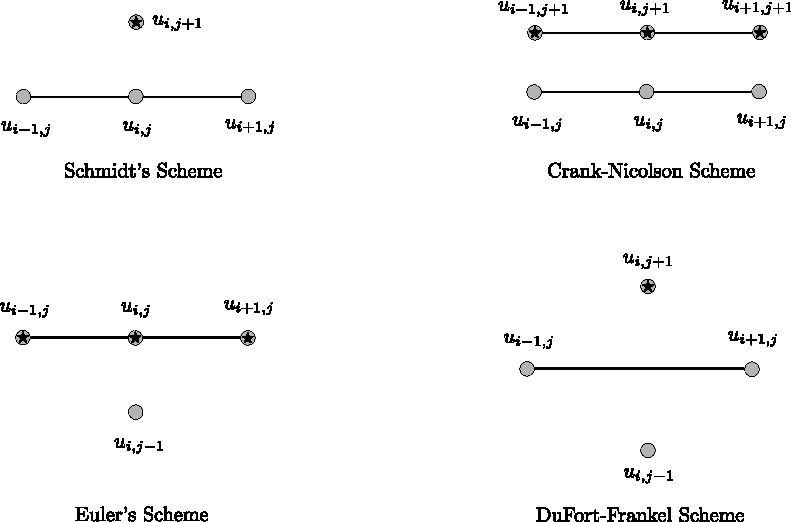
\includegraphics[width=\textwidth]{HeatEquationSchemes.pdf}
    \caption{Computational Stencils for various schemes for Heat Equation.}
    \label{fig:HES}
\end{figure}
Consider one-dimensional heat equation of the form
\begin{equation}
    \begin{split}
        \pder{U}{t} &= \pder{^2U}{x^2}\;\;x \in(0,1)\;,\;\;t>0\\
        U(0,t) &= U(1,t) = 0\;,\;\;t> 0 \;\;\text{(Boundary Condition)}\\
        U(x,0) &= f(x)\;,\;\;0\le x \le 1\;\;\text{(Initial Condition)}
    \end{split}
\end{equation}
Set $x_i = ih\;,\;\;i=0,1,2,\dots$ and $t_j = jk\;,\;\;j=0,1,2,\dots$.
\nll
Let $U_{ij}$ be the \textbf{true value of the solution} at the grid point $(x_i,t_j)$. 
\nll
Let $u_{ij}$ be the \textbf{finite difference approximation to the true solution} at $(x_i,t_j)$. Thus,
\[ u_{ij} \approx U_{ij} = U(x_i,t_j) \]
with the basic notations in hand, we now explain various schemes by which one can approximate the partial derivative with the help of finite differences.
\subsection{Schmidt's Explicit Scheme}
\textbf{Technique : }Use the \textbf{forward-time and central-space (FTCS)} schemes to approximate $\pder{U}{t} = \pder{^2U}{x^2}$ at the grid point $(x_i,t_j)$.
\nll
Hence, we would get the partial derivatives as (from Eq. 14.8),
\begin{equation}
    \begin{split}
        \left(\pder{U}{t}\right)_{(x_i,t_j)} &\approx \frac{u_{i,j+1} - u_{i,j}}{k} \\
        \left( \pder{^2 U}{x^2} \right)_{(x_i,t_j)} &\approx \frac{u_{i+1,j} - 2u_{i,j} + u_{i-1,j}}{h^2}
    \end{split}
\end{equation}
With the above approximations to the derivatives, the heat equation 14.9 would thus yield to the following,
\begin{equation*}
    \begin{split}
        \frac{u_{i,j+1} - u_{i,j}}{k} &= \frac{u_{i+1,j} - 2u_{i,j} + u_{i-1,j}}{h^2}
    \end{split}
\end{equation*}
which on simplification gives,
\begin{equation}
    \begin{split}
        u_{i,j+1} &= ru_{i-1,j} + (1-2r)u_{i,j} + ru_{i+1,j}\\
        &\text{where,}\\
        r &= \frac{k}{h^2}
    \end{split}
\end{equation}
Note that in this equation, we want values of $u$ at different values of $t$ as the values of $u$ at different values of $x$ for a fixed $t$ can be found by recursively using Eq. 14.11, the Boundary conditions and Initial conditions.
\nll
\textbf{Remarks:}
\begin{itemize}
    \item {It is a two level \textbf{explicit system} as the solution at the $j^{th}$ level is only computed by values at the $j-1^{th}$ level.}
    \item{This scheme is \textbf{conditionally stable} when $\left( 0 < r \le \frac{1}{2} \right)$ (will be proved soon).}
    \item{The local truncation error is $O(h^2) + O(k)$ as seen from Eq. 14.9.}
\end{itemize}
\subsection{Euler's Implicit Scheme}
\textbf{Technique : }Use the \textbf{backward-time and central-space (BTCS)} schemes at the point $(x_i,t_j)$.
\nll
The approximations thus are,
\begin{equation}
    \begin{split}
        \left(\pder{U}{t}\right)_{(x_i,t_j)} &\approx \frac{u_{i,j} - u_{i,j-1}}{k}\\
        \left( \pder{^2 U}{x^2} \right)_{(x_i,t_j)} &\approx \frac{u_{i+1,j} - 2u_{i,j} + u_{i-1,j}}{h^2}
    \end{split}
\end{equation}
Thus the heat equation is,
\begin{equation*}
     \frac{u_{i,j} - u_{i,j-1}}{k} = \frac{u_{i+1,j} - 2u_{i,j} + u_{i-1,j}}{h^2}
\end{equation*}
and on simplification, it yields,
\begin{equation}
\begin{split}
    u_{i,j-1} &= -ru_{i-1,j} + (1+2r)u_{i,j} - ru_{i+1,j} \\
    &\text{where,}\\
    r &= \frac{k}{h^2}
    \end{split}
\end{equation}
\textbf{Remarks:}
\begin{itemize}
    \item{It is a two-level \textbf{implicit scheme}.}
    \item{At each time level, we are required to solve a linear system.}
    \item{This scheme is \textbf{unconditionally stable}, that is, it's stable for all values of $r$.}
    \item{The local truncation error is $O(h^2) + O(k)$.}
\end{itemize}
\subsection{Crank-Nicolson Scheme}
\textbf{Technique : }Use the central difference formula for both time and space at the mid point of on time scale.
\nll
\begin{equation}
    \begin{split}
        \left( \pder{U}{t} \right)_{\left(x_i,t_{j+\frac{1}{2}}\right)} &\approx \frac{u_{i,j+1} - u_{i,j}}{k}\;\;\text{(From Eq. 9.15)}\\
        \left( \pder{^2U}{x^2} \right)_{\left(x_i,t_{j+\frac{1}{2}}\right)} &\approx \frac{1}{2}\left[ \frac{u_{i-1,j+1}-2u_{i,j+1} + u_{i+1,j+1}}{h^2} + \frac{u_{i-1,j} - 2u_{i,j} + u_{i+1,j}}{h^2}\right]
    \end{split}
\end{equation}
Thus the Heat equation gives us,
\begin{equation*}
    \frac{u_{i,j+1} - u_{i,j}}{k} = \frac{1}{2}\left[ \frac{u_{i-1,j+1}-2u_{i,j+1} + u_{i+1,j+1}}{h^2} + \frac{u_{i-1,j} - 2u_{i,j} + u_{i+1,j}}{h^2}\right]
\end{equation*}
Simplifying this finally gives us,
\begin{equation}
-ru_{i-1,j+1} + (2+2r)u_{i,j+1} - ru_{i+1,j+1} = ru_{i-1,j} + (2-2r)u_{i,j} + ru_{i+1,j}
\end{equation}
where $r = \frac{k}{h^2}$.
\nll
\textbf{Remarks:}
\begin{itemize}
    \item{As visible, this is a two-level \textbf{implicit scheme} as the value at level $j+1$ and level $j$ are interlinked in the different levels of $i$. In-short, the $j+1$ level is in multiple places with different levels of $i$.}
    \item{At each time level, we are required to solve a linear system.}
    \item{This scheme is also \textbf{unconditionally stable}.}
    \item{The local truncation error is $O(h^2) + O(k^2)$ (From Eq. 9.15).}
\end{itemize}
\subsection{Richardson's Scheme}
\textbf{Technique : }Use only the central-time and central-space (CTCS) approximation.
\nll
The CTCS approximations are (follows from Eq. 9.15),
\begin{equation}
    \begin{split}
        \left(\pder{U}{t}\right)_{(x_i,t_j)} &\approx \frac{u_{i,j+1} - u_{i,j-1}}{2k}\\
        \left( \pder{^2U}{x^2}\right)_{(x_i,t_j)} &\approx \frac{u_{i-1,j} -2u_{i,j} + u_{i+1,j}}{h^2}
    \end{split}
\end{equation}
the heat equation thus gives us,
\begin{equation}
    \frac{u_{i,j+1} - u_{i,j-1}}{2k} =  \frac{u_{i-1,j} -2u_{i,j} + u_{i+1,j}}{h^2}
\end{equation}
\textbf{Remarks:}
\begin{itemize}
    \item {It is a three level \textbf{explicit scheme} .}
    \item{This scheme is \textbf{unstable}, thus not used practically.}
    \item{Local truncation error is $O(h^2) + O(k^2)$.}
\end{itemize}
\subsection{DuFort-Frankel Explicit Scheme}
\textbf{Technique : }Modification of Richardson's scheme as follows,
\begin{equation}
    u_{i,j} = \frac{u_{i,j-1}  +  u_{i,j+1}}{2}
\end{equation}
Thus, substituting in the Heat equation and further simplification yields,
\begin{equation}
    u_{i,j+1} = \frac{1-2r}{1+2r} u_{i,j-1} + \frac{2r}{1+2r} (u_{i-1,j} + u_{i+1,j})
\end{equation}
\textbf{Remarks:}
\begin{itemize}
    \item {It is a three level \textbf{explicit scheme}.}
    \item{This scheme is \textbf{unconditionally stable}.}
    \item{The local truncation error is $O(h^2) + O(k^2)$.}
\end{itemize}
\subsection{Weighted Average Approximation}
A more \textbf{general finite-difference approximation to the heat equation} is given by
\begin{equation}
    \begin{split}
        \frac{u_{i,j+1} - u_{i,j}}{k} = & \frac{1}{h^2} \left[ \theta(u_{i-1,j+1} - 2u_{i,j+1} + u_{i+1,j+1}) + (1-\theta)(u_{i-1,j} - 2u_{i,j} + u_{i+1,j}) \right]
    \end{split}
\end{equation}
where $\theta$ is a parameter such that $0 \le \theta \le 1$.
\nll
Now observe that it generalises the previous methods,
\begin{equation}
    \begin{split}
        \theta &= 0 \;\;\implies\;\;\text{Scheme's Explicit Scheme}\\
        \theta &= 1 \;\;\implies\;\;\text{Euler's Implicit Scheme}\\
        \theta &= \frac{1}{2} \;\;\implies\;\;\text{Crank-Nicolson Scheme}
    \end{split}
\end{equation}
\textbf{Remarks:}
\begin{itemize}
    \item {This scheme is \textbf{unconditionally stable} for $\frac{1}{2}\le \theta \le 1$.}
    \item{Also, this scheme is \textbf{conditionally stable} for $0\le \theta < \frac{1}{2}$. The condition for stability is,
    \[r = \frac{k}{h^2} \le \frac{1}{2(1-2\theta)}\]
    }
\end{itemize}
Now, define the central-difference operators $\delta_x$ and $\delta_t$ as:
\begin{equation}
    \begin{split}
        \delta_x \phi_{i,j} &= \phi_{i+\frac{1}{2},j} - \phi_{i-\frac{1}{2},j}\\
        \delta_t \phi_{i,j} &= \phi_{i,j+\frac{1}{2}} - \phi_{i,j-\frac{1}{2}}
    \end{split}
\end{equation}
Thus, we can write the explicit scheme for heat equation as,
\begin{equation}
    \begin{split}
        \delta_tu_{i,j+\frac{1}{2}} &= u_{i,j+1} - u_{i,j}\\
        \delta_x (\delta_x u_{i,j}) &= \delta_x(u_{i+\frac{1}{2},j} - u_{i-\frac{1}{2},j} )\\
        &= u_{i+1,j} - 2u_{i,j} + u_{i-1,j}
    \end{split}
\end{equation}
and finally,
\begin{equation}
    \frac{1}{k} \delta_t u_{i,j+\frac{1}{2}} = \frac{1}{h^2}\delta_x^2u_{i,j}
\end{equation}
Note that using the definitions in Eq. 14.23, you can write the \textbf{Euler's Implicit scheme} as,
\begin{equation}
    \frac{1}{k} \delta_t u_{i,j-\frac{1}{2}} = \frac{1}{h^2} \delta_x^2 u_{i,j}
\end{equation}
the \textbf{Crank-Nicolson scheme},
\begin{equation}
    \frac{1}{k}\delta_t u_{i,j+\frac{1}{2}} = \frac{1}{2h^2} \left[ \delta_x^2u_{i,j+1} + \delta_x^2 u_{i,j}\right]
\end{equation}
and finally, the\textbf{ Weighted Average scheme},
\begin{equation}
    \frac{1}{k}\delta_t u_{i,j+\frac{1}{2}} = \frac{1}{h^2}\left[ \theta \delta_x^2 u_{i,j+1} + (1-\theta) \delta_x^2 u_{i,j} \right]
\end{equation}
\section{Consistency \& Stability of Finite Difference Equations}
To discuss the stability of the schemes discussed earlier, we now formulate the definitions needed for calculating that.
\nll
Let
\begin{equation}
    L(U) = 0
\end{equation}
represent the partial differential equation in the independent variables $x$ and $t$ with exact solution $U$. Let,
\begin{equation}
    F_{i,j} (u) = 0
\end{equation}
represent the finite difference equation approximation for the PDE at $(i,j)^{th}$ mesh point with exact solution $u$.
\nll
The local truncation error $T_{i,j}(U)$ at the point $(ih,jk)$ is defined by
\[T_{i,j}(U) = F_{i,j}(U) - L(U_{i,j}) = F_{i,j}(U)\]
as $L(U_{i,j}) = 0$. Thus, $T_{i,j}$ gives an indication of the error resulting from the replacement of $L(U_{i,j})$ by $F_{i,j}(U)$. We hence arrive at the following definition,
\nll
\defin  \;:  \tit{If $T_{i,j} (U) \to 0$ as $h\to 0$ and $k\to 0$, then the difference equation in Eq. 14.29 is said to be \textbf{consistent} or \textbf{compartible} with the PDE Eq. 14.28.}
\nll
\textbf{Example.} To illustrate the use of this definition, let us, for example, consider the local truncation error $T_{i,j}$ of the two level explicit scheme approximating $U_t = U_{xx}$ at the point $(ih,jk)$.
\nll
The finite difference equation in this case will be (Eq. 14.11),
\[F_{i,j}(u) = \frac{u_{i,j+1} - u_{i,j}}{k} - \frac{u_{i-1,j} - 2u_{i,j} + u_{i+1,j}}{h^2}= 0\]
thus the Truncation error $T_{i,j}$,
\begin{equation}
    T_{i,j}(U) = F_{i,j}(U) = \frac{U_{i,j+1} - U_{i,j}}{k} - \frac{U_{i-1,j} - 2U_{i,j} + U_{i+1,j}}{h^2}
\end{equation}
By Taylor's Expansion,
\begin{equation}
\begin{split}
    U_{i+1,j} &= U((i+1)h,j) = U(x_i + h,t_j)\\
    &= U_{i,j} + h\bpder{U}{x}{i,j} + \frac{h^2}{2} \bpder{^2U}{x^2}{i,j} + \frac{h^3}{3!} \bpder{^3U}{x^3}{i,j} + \dots\\
    U_{i-1,j} &= U(x_i - h,t_j)\\
    &= U_{i,j} - h\bpder{U}{x}{i,j} + \frac{h^2}{2} \bpder{^2U}{x^2}{i,j} - \frac{h^3}{3!} \bpder{^3U}{x^3}{i,j} + \dots\\
    U_{i,j+1} &= U(x_i,t_j + k)\\
    &= U_{i,j} + k\bpder{U}{t}{i,j} + \frac{k^2}{2} \bpder{^2U}{t^2}{i,j} + \frac{k^3}{3!} \bpder{^3U}{t^3}{i,j} + \dots
\end{split}
\end{equation}
Substituting these approximations in the Finite Difference Eq. 14.30, we get,
\begin{equation*}
    \begin{split}
        T_{i,j} &= \left( \pder{U}{t} - \pder{^2U}{x^2} \right)_{i,j} + \frac{1}{2}k\bpder{^2U}{t^2}{i,j} - \frac{1}{12} h^2\bpder{^4U}{x^4}{i,j} + \frac{1}{6}k^2\bpder{^3U}{t^3}{i,j} - \frac{1}{360}h^4\bpder{^6U}{x^6}{i,j} + \dots
    \end{split}
\end{equation*}
Note that since $\left( \pder{U}{t} - \pder{^2U}{x^2} \right)_{i,j} = 0$, the major contribution to the local truncation error happen only through the following term,
\[\frac{1}{2}k\bpder{^2U}{t^2}{i,j} - \frac{1}{12} h^2\bpder{^4U}{x^4}{i,j}\]
Therefore, $T_{i,j} = O(k) + O(h^2)$. Also note that,
\[\boxed{T_{i,j} \to 0 \;\;\text{as}\;\; h\to 0\;\text{and}\;k\to 0}\]
Thus, the explicit scheme approximating the heat equation in Eq. 14.11 is \textbf{consistent} with the heat equation.
\section{Stability}
\defin \;: \tit{Stability is related to the round-off error. We say that the scheme is \textbf{stable} if the round-off error in the numerical process is bounded.}
\nll
Let $R = \left\{ (x,t) \vert 0\le x\le 1\;,\;\; 0\le t\le T \right\}$ be a rectangle. Consider the PDE,
\[ L(U) = 0 \;\;\text{in}\;\;R\]
with prescribed initial and boundary conditions. 
\nll
Let $h$ and $k$ be the mesh parameters such that,
\begin{equation*}
    \begin{split}
        x_i &= ih\;,\;\;i=0,1,\dots,N\;\text{with}\;Nh=1\\
         t_j &= jk\;,\;\;j=0,1,\dots,N\;\text{with}\;Jk=T
    \end{split}
\end{equation*}
Assume that $h$ is related to $k$ as follows: As $h\to 0$, then $k\to 0$ (or $k=O(h)$ or $k=O(h^2)$).
\nll
Consider the \textbf{general finite difference approximation of the form}:
\begin{equation}
    b_{i-1}u_{i-1,j+1} + b_iu_{i,j+1} + b_{i+1}u_{i+1,j+1} = c_{i-1}u_{i-1,j} + c_iu_{i,j} + c_{i+1}u_{i+1,j}
\end{equation}
where $b_i$'s and $c_i$'s are constants.
\nll
Now, \textbf{suppose that the boundary values $u_{0,j}$ and $u_{N,j}$ for $j>0$ are known}. Then for remaining $i=1,\dots,N-1$, we can write,
\begin{equation}
    \begin{split}
        &\begin{bmatrix}
            b_1 & b_2 &  &  &  \\
            b_1 & b_2 & b_3 &  &  \\
            \ddots & \ddots & \ddots  &  &  \\
             &  &b_{N-3}  & b_{N-2} &b_{N-1}  \\
              &  &  & b_{N-2} & b_{N-1} 
        \end{bmatrix} \begin{bmatrix}
            u_{1,j+1}\\
            u_{2,j+1}\\
            \vdots\\
            u_{N-2,j+1}\\
            u_{N-1,j+1}
        \end{bmatrix}\\
        &=  \begin{bmatrix}
            c_1 & c_2 &  &  &  \\
            c_1 & c_2 & c_3 &  &  \\
            \ddots & \ddots & \ddots  &  &  \\
             &  &c_{N-3}  & c_{N-2} &c_{N-1}  \\
              &  &  & c_{N-2} & c_{N-1} 
        \end{bmatrix} \begin{bmatrix}
            u_{1,j}\\
            u_{2,j}\\
            \vdots\\
            u_{N-2,j}\\
            u_{N-1,j}
        \end{bmatrix}+
         \begin{bmatrix}
            c_0u_{0,j} - b_0u_{0,j+1}\\
            0\\
            \vdots\\
            0\\
            c_Nu_{N,j} - b_Nu_{N,j+1}
        \end{bmatrix}
    \end{split}
\end{equation}
In matrix notation,
\begin{equation}
    \begin{split}
        \mat{B}\vect{u}_{j+1} &= \mat{C}\vect{u}_{j} + \vect{d}_j\\
\implies \vect{u}_{j+1} &= \mat{B}^{-1}\mat{C}\vect{u}_j + \mat{B}^{-1} \vect{d}_j\\
\implies \vect{u}_{j+1} &= \mat{A}\vect{u}_j + \vect{f}_j
    \end{split}
\end{equation}
where $\mat{A} = \mat{B}^{-1}\mat{C}$ and $\vect{f}_j = \mat{B}^{-1}\vect{d}_j$.
\nll
We can apply the Eq. 14.34 recursively to obtain
\begin{equation}
    \begin{split}
        \vect{u}_j &= \mat{A}\vect{u}_{j-1} + \vect{f}_{j-1} \\
        &= \mat{A}(\mat{A}\vect{u}_{j-2} + \vect{f}_{j-2}) + \vect{f}_{j-1} = \mat{A}^2\vect{u}_{j-2} + \mat{A}\vect{f}_{j-2} + \vect{f}_{j-1}\\
        &= \dots\\
        &= \mat{A}^j\vect{u}_0 +  \mat{A}^{j-1}\vect{f}_0 +  \mat{A}^{j-2}\vect{f}_1 + \dots + \vect{f}_{j-1}
    \end{split}
\end{equation}
$\boxed{\star}$ where $\vect{u}_0$ is the \textbf{vector of initial values} and $\vect{f}_0,\vect{f}_1,\dots,\vect{f}_{j-1}$ are the \textbf{vectors of known boundary values}.
\nll
Since we want to find the stability of the finite difference method, so we check the error in the resultant vector after \textbf{perturbing the initial value from $\vect{u}_0$ to $\vect{u}_0^*$}. Thus, the exact solution at the $j^{th}$ time level will be,
\begin{equation}
  \vect{u}_j^* = \mat{A}^j\vect{u}_0^* +  \mat{A}^{j-1}\vect{f}_0 +  \mat{A}^{j-2}\vect{f}_1 + \dots + \vect{f}_{j-1}
\end{equation}
Now, define the \textbf{perturbation error} by 
\[\vect{e}^* = \vect{u}^* - \vect{u}\]
then it follows from Eq. 14.35 and 14.36 that,
\[\vect{e}_j = \vect{u}_j^* - \vect{u}_j = \mat{A}(\vect{u}_0^* - \vect{u}_0) = \mat{A}^j\vect{e}_0\]
where $\vect{e}_0$ is the amount by which the initial value $\vect{u}_0$ is perturbed by.
\nll
Note that,
\begin{equation}
    \norm{\vect{e}_j} = \norm{\mat{A}^j\vect{e}_0} \le \norm{\mat{A}^j}\norm{\vect{e}_0}
\end{equation}
Now if there exists a positive number $M$, independent of $j,h$ and $k$ such that $\norm{\mat{A}^j} \le M$, then it's easy to see that,
\[\norm{\vect{e}_j} \le M\norm{\vect{e}_0}\]
Now to use this, first note that,
\[\norm{\mat{A}^j} = \norm{\mat{A}^{j-1}\mat{A}}\le \norm{\mat{A}^{j-1}}\norm{\mat{A}}\le \dots\le \norm{\mat{A}}^j\]
Thus, the bound $M$ on $\norm{\mat{A}^j}$ would imply that,
\begin{equation*}
\begin{split}
    \norm{\vect{e}_j} &\le \norm{\mat{A}}^j\norm{\vect{e}_0}
    \end{split}
\end{equation*}
The \textbf{Lax \& Richtmeyer definition of stability} thus requires that
\begin{equation}
\boxed{    \norm{\mat{A}} \le 1}
\end{equation}
This is the \textbf{necessary and sufficient condition} for the difference equations to be \textbf{stable} when the solution of the PDE does not increase as $t$ increases. 
\section{Stability Analysis by Matrix Method}
Now that we have converted our problem to equivalent matrix formulation, we can now use a lot of techniques for checking convergence and stability available from Matrix Theory! 
\nll
In particular, we would explore stability of finite difference equations by two methods, namely \textbf{Matrix method} and \textbf{von Neumann's\footnote{\textit{Of-course!}} method}.
\nll
Before that, we present brief review of matrix theory.
\subsection{Basic Elements of Matrix Theory}
\begin{itemize}
    \item {Let $\mat{A}$ be an $n\times n$ matrix. Define,
    \begin{equation}
        \begin{split}
            \norm{\mat{A}}_1 &= \underset{1\le j \le n}{\max} \sum_{i=1}^n \abs{a_{ij}}\\ 
            \norm{\mat{A}}_\infty &= \underset{1\le i \le n}{\max} \sum_{j=1}^n \abs{a_{ij}}\\
            \norm{\mat{A}} &= \underset{x\neq 0}{\max} \frac{\norm{\mat{A}\vect{x}}}{\norm{\vect{x}}} = \underset{\norm{x} = 1}{\max} \norm{\mat{A}\vect{x}}
        \end{split}
    \end{equation}
    }
    \item{Let $\vect{v}_1,\vect{v}_2,\dots,\vect{v}_n$ be the eigenvectors corresponding to the eigenvalues $\lambda_1,\lambda_2,\dots,\lambda_n$ of $\mat{A}$. Then,
    \begin{equation}
        \begin{split}
            \mat{A}\vect{v}_i &= \lambda_i \vect{v}_i \\
            \implies\;\;  \norm{\mat{A}\vect{v}_i} &= \norm{\lambda_i \vect{v}_i} = \abs{\lambda_i} \norm{\vect{v}_i}\\
            \implies\;\;\abs{\lambda_i} \norm{\vect{v}_i} &= \norm{\mat{A}\vect{v}_i} \le \norm{\mat{A}}\norm{\vect{v}_i}\\
            \implies\;\; \abs{\lambda_i} &\le \norm{\mat{A}}\;,\;\;i=1,\dots,N\\
            \implies\;\; \underset{i}{\max} \abs{\lambda_i} &\le \norm{\mat{A}}\\
            \text{or,}\;\;\rho(\mat{A}) &\le \norm{\mat{A}}
        \end{split}
    \end{equation}
    where $\rho(\mat{A})$ is called the \textbf{spectral radius} and is the largest eigenvalue of matrix $\mat{A}$.
    }
    \item{The eigenvalues of the following $n\times n$ matrix 
    \begin{equation*}
        \begin{bmatrix}
            a & b &  &  &  \\
            c & a & b &  &  \\
            \ddots & \ddots & \ddots  &  &  \\
             &  &c  & a &b  \\
              &  &  & a & b 
        \end{bmatrix}
    \end{equation*}
    are given by,
    \begin{equation}
        \lambda_s = a+ 2\sqrt{bc}\cos\left( \frac{s\pi}{n+1} \right)\;,\;\;s = 1,\dots,n
    \end{equation}
    where $a,b,c\in \mathbb{R}$.
    }
\end{itemize}
\subsubsection{Lax-Richtmeyer Stability condition}
As in Eq. 14.38, the Lax-Richtemeyer Condition that $\norm{\mat{A}} \le 1$ implies that,
\begin{equation}
\boxed{    \norm{\mat{A}} \le 1 \;\;\implies\;\; \rho(\mat{A}) \le 1}
\end{equation}
\textbf{Note that the converse is not true}, that is, 
\[\rho(\mat{A}) \le 1 \;\;\centernot\implies\;\;\norm{\mat{A}} \le 1\]
However, if $\mat{A}$ is real and symmetric, then
\begin{equation}
\norm{\mat{A}} = \sqrt{\rho(\mat{A}^T\mat{A})} = \sqrt{\rho(\mat{A}^2)} = \sqrt{\rho^2(\mat{A})} = \rho(\mat{A})
\end{equation}
\subsubsection{Stability of the Schmidt's Explicit Scheme}
\[u_{i,j+1} = ru_{i-1,j} + (1-2r)u_{i,j} + ru_{i+1,j}\;,\;\;i=1,\dots,N-1\]
As usual, assuming that the boundary values $u_{0,j}$ and $u_{N,j}$ are known for $j=1,2,\dots$, thus the equivalent matrix formulation becomes,
\begin{equation*}
    \begin{split}
        \begin{bmatrix}
            u_{1,j+1}\\
            u_{2,j+1}\\
            \vdots\\
            u_{N-2,j+1}\\
            u_{N-1,j+1}
        \end{bmatrix} &= \underbrace{\begin{bmatrix}
            (1-2r) & r &  &  &  \\
            r & (1-2r) & r &  &  \\
            \ddots & \ddots & \ddots  &  &  \\
             &  & r & (1-2r) & r \\
              &  &  & r & (1-2r) 
        \end{bmatrix}}_{\mat{A}} \begin{bmatrix}
            u_{1,j}\\
            u_{2,j}\\
            \vdots\\
            u_{N-2,j}\\
            u_{N-1,j}
        \end{bmatrix} + \begin{bmatrix}
            ru_{0,j}\\
            0\\
            \vdots\\
            0\\
            ru_{N,j}
        \end{bmatrix}
    \end{split}
\end{equation*}
Clearly, the amplification matrix is $\mat{A}$.
\nll
Now, note that 
\[\norm{\mat{A}}_\infty = 2\abs{r} + \abs{1-2r}\]
Now,
\begin{itemize}
    \item[\textbf{CASE I : }]{$1-2r \ge 0 \;\implies\; 0\le r\le \frac{1}{2}$.
    \nll
    Note that,
    \[\norm{\mat{A}}_\infty = r+ 1-2r +r = 1\]
    } 
    \item[\textbf{CASE II : }]{$1-2r < 0 \; \implies\; r > \frac{1}{2}$.
    \nll
    Therefore, $\abs{1-2r} = 2r-1$, and
    \[\norm{\mat{A}}_\infty = r+ 2r-1 + r = 4r-1 > 1\]
    }
\end{itemize}
\textbf{Thus, the scheme is stable only for $0<r\le \frac{1}{2}$}. Note that since $\mat{A}$ is real and symmetric,
\[\norm{\mat{A}} = \rho(\mat{A}) = \underset{s}{\max} \abs{\mu_s}\]
where $\mu_s$ is the $s^{th}$ eigenvalue of $\mat{A}$.
\nll
We can do the same calculation in a more\textit{ eigenvalue oriented }one, i.e., deriving a general form of eigenvalue and using Lax-Richtemeyer condition of stability in Eq. 14.42.
\nll
For this, first note that the matrix $\mat{A}$ can be rewritten as,
\[\mat{A} = \mat{I}_{N-1} + r\mat{T}_{N-1}\]
where,
\begin{equation}
\begin{split}
   \mat{I}_{N-1} &= \begin{bmatrix}
            1 &  &  &  &  \\
             & 1 &  &  &  \\
             & & \ddots  &  &  \\
             &  &  & 1 &  \\
              &  &  &  & 1 
        \end{bmatrix}\\
    \mat{T}_{N-1} &= \begin{bmatrix}
            -2 & 1 &  &  &  \\
            1 & -2 & 1 &  &  \\
              &  & \ddots  &  &  \\
             &  & 1 & -2 & 1 \\
              &  &  & 1 & -2
        \end{bmatrix}
\end{split}
\end{equation}
Now, a particular eigenvalue of $\mat{A}$ is just the sum of the corresponding eigenvalues of $\mat{I}_{N-1}$ and $\mat{T}_{N-1}$. Thus, we first need to find the eigenvalues $\lambda_s$ of $\mat{T}_{N-1}$ as the eigenvalues of $\mat{I}_{N-1}$ are trivially all 1.
\begin{equation*}
    \begin{split}
    \lambda_s &= -2 + 2\cos\left( \frac{s\pi}{N} \right) \;\;\text{(Eq. 14.41)}\\
    &= -4\sin^2\left(\frac{s\pi}{2N}\right)
    \end{split}
\end{equation*}
for $s = 1,\dots,N-1$. Therefore, the eigenvalues of $\mat{A}$ are,
\begin{equation}
    \mu_s = 1-4r\sin^2\left(\frac{s\pi}{2N}\right)
\end{equation}
Now, for the stability, $\rho(\abs{\mu_s}) \le 1$, 
\begin{equation}
    \begin{split}
		\rho(\abs{\mu_s}) = \underset{s}{\max}\abs*{1-4r\sin^2\left(\frac{s\pi}{2N}\right)}&\le 1
    \end{split}
\end{equation}
which leads to,
\begin{equation*}
	\begin{split}
		-1&\le 1-4r\sin^2\left(\frac{s\pi}{2N}\right) \le 1\\
	\implies r&\le	\frac{1}{2\sin^2\left(\frac{s\pi}{2N}\right)}
	\end{split}
\end{equation*}
which implies that (for $s=N-1$),
\begin{equation}
	\begin{split}
		r\le \frac{1}{2\sin^2\left(\frac{(N-1)\pi}{2N}\right)}
	\end{split}
\end{equation}
Hence, for $h\to 0$, then $N\to \infty$, which then implies that $\sin^2\left(\frac{(N-1)\pi}{2N}\right) \to 1$. Which implies that,
\begin{equation}
	r\le \frac{1}{2}
\end{equation}
is the required condition for stability (conditionally).

\section{Stability Analysis by von Neumann Method \& Lax Equivalence Theorem}
We previously saw the basic definition of stability by Lax-Richtmeyer condition. Now, we shift our focus on extending this criterion for checking the stability of any given finite difference approximation of a certain IVP through a method called \textit{von Neumann stability method}.
\nll
Consider the IVP,
\begin{equation}
	\begin{split}
		U_t &= U_{xx} \;,\;\;0\le x\le L\;,\;\;0<t\le T\\
		U(x,0) &= f(x) \;,\;\;0\le x\le L
	\end{split}
\end{equation}
The basic idea now followed to find an approximate solution to this is two-fold:
\begin{itemize}
	\item[$\boxed{\star}$]{Express initial data by finite Fourier series along the initial mesh-point at $t=0$.}
	\item[$\boxed{\star}$]{Study the growth of a function that reduced to this series at $t=0$ by variable separation method.}
\end{itemize}
Hence, the Fourier series in complex exponential form can be represented as,
\[U(x,0) = f(x) = \sum A_n e^{\frac{i\pi nx}{L}}\]
Now, let us introduce the commonly used notations for this method before moving into it's peculiarities,
\nll
\textbf{Define},
\begin{equation}
	\begin{split}
		x_p &= ph\;,\;\;p=0,1,2,\dots,N\;\text{with}\;Nh = L\\
		t_q &= qk\;,\;\;q=0,1,2,\dots,J\;\text{with}\;Jk = T\\
		u(x_p,t_q) &= u_{p,q} = u(ph,qk)
	\end{split}
\end{equation}
With the above, first note that the Fourier Series terms at particular values of $x_p$ are
\[A_ne^{\frac{i\pi n x_p}{L}} = A_ne^{\frac{i\pi nph}{Nh}} = A_ne^{i\beta_n ph}\;\;\text{where}\;\;\beta_n = \frac{\pi n}{Nh}\]
Now, at $q=0$, i.e. $t = t_0 = 0$,
\[u_{p,0} = u(ph,0) = \sum_{n=0}^NA_ne^{i\beta_nph}\]
Using the given $u_{p,0}$ at $p=0,1,2,\dots,N$, \textbf{the constants $A_n$ can be uniquely determined}! But since this problem is a linear one, thus it is enough to investigate the propagation of only one initial value, such as $e^{i\beta ph}$ as separate solutions are additive. The coefficient $A_n$ is a constant and can be neglected for the growth analysis. Thus, we study,
\begin{equation}
	u_{p,q} = e^{i\beta ph} \cdot e^{\alpha qk} = e^{i\beta ph}\cdot \xi^q
\end{equation}
where $\boxed{\xi = e^{\alpha k}}$ and $\alpha$ is a constant. Note that this turns to $e^{i\beta ph}$ at $k=0$ which corresponds to the $t=0$ criterion.
\nll
Now,\textbf{ by Lax-Richtemeyer definition of stability}, we have,
\[\abs*{u_{p,q}} \le C\;\;\forall q\le J\]
as $h\to0$, $k\to 0$ and for all values of $\beta$ needed to satisfy the initial conditions. This inequality directly translate to,
\begin{equation}
	\begin{split}
		\abs*{u_{p,q}} &\le C\\
		\abs*{e^{i\beta ph}\cdot \xi^p} &\le C \;\;\;\text{(Eq. 14.51)}\\
		\abs*{e^{i\beta ph}}\abs*{\xi^p} &\le C\\
		\abs*{\xi^p} &\le C
	\end{split}
\end{equation}
i.e. $\abs{\xi^p}$ should remain bounded, which is only possible if
\begin{equation}
	\boxed{\xi\le 1}
\end{equation}
which is the \textbf{necessary and sufficient condition for stability}, or also called the \textbf{von Neumann stability} condition.
\nll
\textbf{Remarks:}
\begin{itemize}
	\item{\textbf{Consistency} is related to the truncation error. We say a finite difference scheme is consistent with given PDE if the truncation error $T_{i,j}\to 0$ as $h\to 0$ and $k\to 0$.}
	\item{Whereas \textbf{Stability} is related to the round-off error. We say that a finite difference scheme is stable if the exact solution of the finite difference equation does not grow with time.}
\end{itemize}
We finally note the major theme of the whole discussion. Since from the beginning, we wanted to find an approximation as \textit{close} as possible to the true solution of an PDE, we hence discuss the \tit{convergence} of the finite difference approximation to the true solution, starting from the following definition.
\nll
\defin\; : \textit{Let $U_{i,j}$ be the exact solution of the PDE at the mesh point $(ih,jk)$ and let $u_{i,j}$ be it's finite difference approximation at the same point. Then, we say that $u_{i,j}$ \textbf{converges} to $U_{i,j}$ if
\[\abs*{u_{i,j} - U_{i,j}} \to 0\;\;\text{as}\;h\to 0 \;\text{and}\;k\to 0\]
}
In the final note, we arrive at the following theorem.
\nll
\theor{16} :\;(\textbf{Lax-Equivalence Theorem}) \textit{Given a well-posed, linear initial value problem and a \textbf{consistent} linear finite difference equation approximating it. Then, \textbf{stability is the necessary \& sufficient condition for convergence}. That is, for a consistent finite difference scheme,
\[\text{Consistency} + \text{Stability} \implies \text{Convergence}\]
}
\newpage
\thispagestyle{empty}
\chapterendsymbol

\end{document}
















